% Options for packages loaded elsewhere
\PassOptionsToPackage{unicode}{hyperref}
\PassOptionsToPackage{hyphens}{url}
%
\documentclass[
  ngerman,
]{book}
\usepackage{lmodern}
\usepackage{amsmath}
\usepackage{ifxetex,ifluatex}
\ifnum 0\ifxetex 1\fi\ifluatex 1\fi=0 % if pdftex
  \usepackage[T1]{fontenc}
  \usepackage[utf8]{inputenc}
  \usepackage{textcomp} % provide euro and other symbols
  \usepackage{amssymb}
\else % if luatex or xetex
  \usepackage{unicode-math}
  \defaultfontfeatures{Scale=MatchLowercase}
  \defaultfontfeatures[\rmfamily]{Ligatures=TeX,Scale=1}
\fi
% Use upquote if available, for straight quotes in verbatim environments
\IfFileExists{upquote.sty}{\usepackage{upquote}}{}
\IfFileExists{microtype.sty}{% use microtype if available
  \usepackage[]{microtype}
  \UseMicrotypeSet[protrusion]{basicmath} % disable protrusion for tt fonts
}{}
\makeatletter
\@ifundefined{KOMAClassName}{% if non-KOMA class
  \IfFileExists{parskip.sty}{%
    \usepackage{parskip}
  }{% else
    \setlength{\parindent}{0pt}
    \setlength{\parskip}{6pt plus 2pt minus 1pt}}
}{% if KOMA class
  \KOMAoptions{parskip=half}}
\makeatother
\usepackage{xcolor}
\IfFileExists{xurl.sty}{\usepackage{xurl}}{} % add URL line breaks if available
\IfFileExists{bookmark.sty}{\usepackage{bookmark}}{\usepackage{hyperref}}
\hypersetup{
  pdftitle={Wahrscheinlichkeiten},
  pdflang={de},
  hidelinks,
  pdfcreator={LaTeX via pandoc}}
\urlstyle{same} % disable monospaced font for URLs
\usepackage{longtable,booktabs}
\usepackage{calc} % for calculating minipage widths
% Correct order of tables after \paragraph or \subparagraph
\usepackage{etoolbox}
\makeatletter
\patchcmd\longtable{\par}{\if@noskipsec\mbox{}\fi\par}{}{}
\makeatother
% Allow footnotes in longtable head/foot
\IfFileExists{footnotehyper.sty}{\usepackage{footnotehyper}}{\usepackage{footnote}}
\makesavenoteenv{longtable}
\usepackage{graphicx}
\makeatletter
\def\maxwidth{\ifdim\Gin@nat@width>\linewidth\linewidth\else\Gin@nat@width\fi}
\def\maxheight{\ifdim\Gin@nat@height>\textheight\textheight\else\Gin@nat@height\fi}
\makeatother
% Scale images if necessary, so that they will not overflow the page
% margins by default, and it is still possible to overwrite the defaults
% using explicit options in \includegraphics[width, height, ...]{}
\setkeys{Gin}{width=\maxwidth,height=\maxheight,keepaspectratio}
% Set default figure placement to htbp
\makeatletter
\def\fps@figure{htbp}
\makeatother
\setlength{\emergencystretch}{3em} % prevent overfull lines
\providecommand{\tightlist}{%
  \setlength{\itemsep}{0pt}\setlength{\parskip}{0pt}}
\setcounter{secnumdepth}{5}
\usepackage{amsthm}
\usepackage{float}
\usepackage{rotating, graphicx}
\usepackage{multirow}
\usepackage{tabularx}
\usepackage{qtree}

% new command for pretty oversets with \sim
\newcommand\simcal[1]{\stackrel{\sim}{\smash{\mathcal{#1}}\rule{0pt}{0.5ex}}}

\newcommand{\comma}{,\,}

\floatplacement{figure}{H}

\PassOptionsToPackage{table}{xcolor}

\usepackage{tcolorbox}

\definecolor{kcblue}{HTML}{D7DDEF}
\definecolor{kcdarkblue}{HTML}{2B4E70}

\makeatletter
\def\thm@space@setup{%
  \thm@preskip=8pt plus 2pt minus 4pt
  \thm@postskip=\thm@preskip
}
\makeatother

% \makeatletter % undo the wrong changes made by mathspec
% \let\RequirePackage\original@RequirePackage
% \let\usepackage\RequirePackage
% \makeatother

\newenvironment{rmdknit}
    {\begin{center}
    \begin{tabular}{|p{0.9\textwidth}|}
    \hline\\
    }
    {
    \\\\\hline
    \end{tabular}
    \end{center}
    }

\newenvironment{rmdnote}
    {\begin{center}
    \begin{tabular}{|p{0.9\textwidth}|}
    \hline\\
    }
    {
    \\\\\hline
    \end{tabular}
    \end{center}
    }

\newtcolorbox[auto counter, number within=section]{keyconcepts}[2][]{%
colback=kcblue,colframe=kcdarkblue,fonttitle=\bfseries, title=Key Concept~#2, after title={\newline #1}, beforeafter skip=15pt}

\ifxetex
  % Load polyglossia as late as possible: uses bidi with RTL langages (e.g. Hebrew, Arabic)
  \usepackage{polyglossia}
  \setmainlanguage[]{german}
\else
  \usepackage[shorthands=off,main=ngerman]{babel}
\fi
\ifluatex
  \usepackage{selnolig}  % disable illegal ligatures
\fi
\usepackage[]{natbib}
\bibliographystyle{apalike}

\title{Wahrscheinlichkeiten}
\author{}
\date{\vspace{-2.5em}}

\begin{document}
\maketitle

{
\setcounter{tocdepth}{1}
\tableofcontents
}
\hypertarget{was-erwartet-dich}{%
\chapter*{Was erwartet dich?}\label{was-erwartet-dich}}
\addcontentsline{toc}{chapter}{Was erwartet dich?}

Ein Distanzlernpfad zum Thema \emph{Wahrscheinlichkeiten}

\hypertarget{aktuelles}{%
\subsection*{Aktuelles}\label{aktuelles}}
\addcontentsline{toc}{subsection}{Aktuelles}

\begin{itemize}
\tightlist
\item
  Stichtag für das Kapitel 3.3 \emph{Baumdiagramme geschickt nutzen} ist der \textbf{26. April}
\end{itemize}

\hypertarget{allgemeine-informationen-zum-ablauf}{%
\subsection*{Allgemeine Informationen zum Ablauf}\label{allgemeine-informationen-zum-ablauf}}
\addcontentsline{toc}{subsection}{Allgemeine Informationen zum Ablauf}

Mit diesem Lernpfad sollst du dir das 4. Kapitel des Schulbuches erarbeiten. Natürlich darfst du das Buch zum Nachlesen und zusätzlichen Üben nutzen. Einige Aufgaben, die hier vorkommen, werden mehr oder weniger aus dem Buch übernommen sein.

Die Arbeit mit einem Lernpfad ist ähnlich der Arbeit mit einem Wochenplan. \textbf{Es gibt Vorgaben, bis wann ein bestimmtes Kapitel oder ein bestimmter Abschnitt durchgearbeitet sein muss.} Und gerade an diesen Stichtagen werden wir vermehrt etwas zusammen durchsprechen. Auch sonst solltest du große Teile deiner Arbeit während der Mathestunden erledigen, da du in diesen ja immer auch die Möglichkeit hast, \textbf{bei Unklarheiten und Verständnisschwierigkeiten nachzufragen.} Natürlich besteht weiterhin die Verpflichtung an den Mathestunden teilzunehmen und \textbf{deine Arbeitsergebnisse am Ende jeder Stunde in OneNote hochzuladen}. Erstelle hierzu bitte immer eine Seite mit dem Tagesdatum als Titel.

Da jede*r von euch über individuelles Vorwissen verfügt, wirst du zum Durcharbeiten dieses Lernpfades nicht genauso lang oder kurz brauchen, wie andere aus deiner Klasse. Es kann sein, dass du auch außerhalb der Mathestunden - also als Hausaufgabe zwischen Mittwoch und Montag - weiterarbeiten musst.

\hypertarget{einfuxfchrung---warum-du-dich-mit-wahrscheinlichkeiten-unbedingt-beschuxe4ftigen-solltest}{%
\chapter{Einführung - Warum du dich mit Wahrscheinlichkeiten unbedingt beschäftigen solltest\ldots{}}\label{einfuxfchrung---warum-du-dich-mit-wahrscheinlichkeiten-unbedingt-beschuxe4ftigen-solltest}}

\href{\%22https://de.wikipedia.org/wiki/Kognitive_Neurowissenschaft\%22}{Kognitive Neurowissenschaftler} bezeichnen das Gehirn gerne als ``Vorhersagemaschine''. Vorhersagen ist demnach allgegenwärtig und wesentliche Funktion des Gehirns. Dabei werden Vorhersagen vor allem dann bewusst, wenn sie nicht eintreffen. Stelle dir zum Beispiel vor, du spielst Tischtennis. Solange der Ball von der Platte wegspringt, wie vorhergesagt, wird dir nicht bewusst, dass du deinen Schläger schon lange, bevor der Ball auf selbigen auftrifft, in Position gebracht hast. Aber wehe auf der Platte liegt ein kleines, unbemerktes Steinchen! Dieses kleine Steinchen macht uns bewusst, dass wir nicht darauf reagieren, wo der Ball ist - das könnten wir gar nicht, die uns bleibende Zeit ist viel zu kurz - , sondern darauf, wohin der Ball unserer Vorhersage zufolge fliegen wird!

So eine Vorhersagemaschine ist für sehr viele Situationen natürlich äußerst praktisch. Sie erleichtert uns den Alltag ungemein. Auch Zukunftsplanungen lassen sich mit ihr machen. Doch wie gut sind wir eigentlich im Vorhersagen?

Bei genauerer Betrachtung müssen wir feststellen, dass wir kaum etwas mit absoluter Sicherheit vorhersagen können. Oft hilft es aber, zumindest über die \textbf{Wahrscheinlichkeit}, mit der ein bestimmtes Ereignis eintritt, gut Bescheid zu wissen. Wie gut wir im Umgang mit solchen Wahrscheinlichkeiten sind, ist also nicht unerheblich! Bedauerlicher Weise müssen wir feststellen, dass wir dabei unter bestimmten Bedingungen recht fehleranfällig zu sein scheinen. Die Psychologie spricht hier auch vom Wahrscheinlichkeitsidioten\ldots.

Wie es um deine Wahrscheinlichkeitseinschätzung bestellt ist, kannst du an den folgenden drei kleinen Aufgaben ausprobieren:

Du bist von den Ergebnissen überrascht? Dann sei gespannt auf mehr.

\hypertarget{vorwissen}{%
\chapter{Vorwissen}\label{vorwissen}}

Wie immer im Matheunterricht baut auch dieses Thema auf bereits gelernten Unterrichtsinhalten auf. Dieses Kapitel soll dir helfen, dich wieder in das Thema ``Wahrscheinlichkeit'' einzufinden und eventuell vorhandene Lücken zu schließen.

\hypertarget{bruchrechnung-kurz-und-knapp}{%
\section{Bruchrechnung kurz und knapp}\label{bruchrechnung-kurz-und-knapp}}

\hypertarget{bruxfcche-kuxfcrzen-und-erweitern}{%
\subsection*{Brüche kürzen und erweitern}\label{bruxfcche-kuxfcrzen-und-erweitern}}
\addcontentsline{toc}{subsection}{Brüche kürzen und erweitern}

Einen Bruch \(a \over b\) mit einer Zahl \(c\) \textbf{erweitern}, bedeutet, dass man \textbf{den Zähler und den Nenner} mit \(c\) \textbf{multipliziert}: \(a \over b\) erweitert mit \(c\) ergibt also \(a \cdot c \over b \cdot c\).

\textbf{Dividiert} man \textbf{Zähler und Nenner} eines Bruches \(x \over y\) durch dieselbe Zahl \(z\), sagt man, \(x \over y\) wird mit \(z\) \textbf{gekürzt}.

Ein Bruch \(e \over f\) heißt \textbf{vollständig gekürzt}, wenn Zähler und Nenner teilerfremd sind. \(2 \over 3\) oder \(1 \over 4\) sind beispielsweise vollständig gekürzt. \(9 \over 15\) dagegen nicht, da man sowohl \(9\) als auch \(15\) durch \(3\) dividieren kann.

\hypertarget{section}{%
\subsubsection*{}\label{section}}
\addcontentsline{toc}{subsubsection}{}

\hypertarget{aufgabe}{%
\subsubsection*{Aufgabe}\label{aufgabe}}
\addcontentsline{toc}{subsubsection}{Aufgabe}

Erweitere \(1 \over 5\) mit \(2\)

\leavevmode\hypertarget{toggleText1}{}%
\(2 \over 10\)

Erweitere \(2 \over 3\) mit \(5\)

\leavevmode\hypertarget{toggleText2}{}%
\(10 \over 15\)

Erweitere \(3 \over 4\) mit \(6\)

\leavevmode\hypertarget{toggleText3}{}%
\(18 \over 24\)

Erweitere \(17 \over 19\) mit \(3\)

\leavevmode\hypertarget{toggleText4}{}%
\(51 \over 57\)

Kürze vollständig: \(8 \over 12\)

\leavevmode\hypertarget{toggleText5}{}%
\(2 \over 3\)

Kürze vollständig: \(8 \over 24\)

\leavevmode\hypertarget{toggleText6}{}%
\(1 \over 3\)

Kürze vollständig: \(72 \over 48\)

\leavevmode\hypertarget{toggleText7}{}%
\(3 \over 2\)

Kürze vollständig: \(21 \over 33\)

\leavevmode\hypertarget{toggleText8}{}%
\(7 \over 11\)

\hypertarget{section-1}{%
\subsubsection*{}\label{section-1}}
\addcontentsline{toc}{subsubsection}{}

\hypertarget{section-2}{%
\subsubsection*{}\label{section-2}}
\addcontentsline{toc}{subsubsection}{}

\hypertarget{bruxfcche-in-dezimalzahlen-oder-prozentangaben-umwandeln}{%
\subsection*{Brüche in Dezimalzahlen oder Prozentangaben umwandeln}\label{bruxfcche-in-dezimalzahlen-oder-prozentangaben-umwandeln}}
\addcontentsline{toc}{subsection}{Brüche in Dezimalzahlen oder Prozentangaben umwandeln}

Möchte man einen Bruch als Dezimalzahl schreiben, muss man den Zähler (schriftlich oder mit Hilfe des Taschenrechners) durch den Nenner dividieren.

Eine Dezimalzahl kann man nun wiederum sehr einfach auch als Prozentzahl angeben: Man verschiebt einfach das Komma um zwei Stellen nach rechts und schreibt hinter die auf diese Weise entstandene Zahl ein \%-Zeichen.

\hypertarget{section-3}{%
\subsubsection*{}\label{section-3}}
\addcontentsline{toc}{subsubsection}{}

\hypertarget{aufgabe-1}{%
\subsubsection*{Aufgabe}\label{aufgabe-1}}
\addcontentsline{toc}{subsubsection}{Aufgabe}

Schreibe als Dezimalzahl\(14 \over 10\)

\leavevmode\hypertarget{toggleText9}{}%
\(1,4\)

Schreibe als Dezimalzahl\(14 \over 100\)

\leavevmode\hypertarget{toggleText10}{}%
\(0,14\)

Schreibe als Dezimalzahl\(12 \over 15\)

\leavevmode\hypertarget{toggleText11}{}%
\(0,8\)

Schreibe als Dezimalzahl\(-{6 \over 4}\)

\leavevmode\hypertarget{toggleText12}{}%
\(-1,5\)

Schreibe in Prozent: \(7 \over 20\)

\leavevmode\hypertarget{toggleText13}{}%
\(35\%\)

Schreibe in Prozent: \(18 \over 48\)

\leavevmode\hypertarget{toggleText14}{}%
\(37,5\%\)

Schreibe in Prozent: \(19 \over 38\)

\leavevmode\hypertarget{toggleText15}{}%
\(50\%\)

Schreibe in Prozent: \(38 \over 19\)

\leavevmode\hypertarget{toggleText16}{}%
\(200\%\)

\hypertarget{section-4}{%
\subsubsection*{}\label{section-4}}
\addcontentsline{toc}{subsubsection}{}

\hypertarget{section-5}{%
\subsubsection*{}\label{section-5}}
\addcontentsline{toc}{subsubsection}{}

\hypertarget{mit-bruxfcchen-rechnen}{%
\subsection*{Mit Brüchen rechnen}\label{mit-bruxfcchen-rechnen}}
\addcontentsline{toc}{subsection}{Mit Brüchen rechnen}

Zwei Brüche werden \textbf{multipliziert}, indem man Zähler mit Zähler und Nenner mit Nenner multipliziert.
\[{a \over b} \cdot {c \over d} = {a \cdot c \over b \cdot d} \]

Durch einen Bruch wird \textbf{dividiert}, indem \textbf{mit seinem Kehrbruch multipliziert} wird.
\[{e \over f} : {x \over y} = {e \cdot y \over f \cdot x}\]

Sollen zwei Brüche \textbf{addiert} oder \textbf{subtrahiert} werden, muss man sie zunächst \textbf{auf den gleichen Nenner bringen}. Anschließend \textbf{addiert} bzw. \textbf{subtrahiert} man die Zähler.

\[{m \over n}+{p \over q} = \frac{m \cdot q}{n \cdot q} + \frac{p \cdot n}{q \cdot n} = {m \cdot q + n \cdot p \over n \cdot q}\]
\[{m \over n}-{p \over q} = \frac{m \cdot q}{n \cdot q} - \frac{p \cdot n}{q \cdot n} = {m \cdot q - n \cdot p \over n \cdot q}\]

\hypertarget{section-6}{%
\subsubsection*{}\label{section-6}}
\addcontentsline{toc}{subsubsection}{}

\hypertarget{aufgabe-2}{%
\subsubsection*{Aufgabe}\label{aufgabe-2}}
\addcontentsline{toc}{subsubsection}{Aufgabe}

\({1 \over 3}\cdot{2 \over 7}\)

\leavevmode\hypertarget{toggleText17}{}%
\(2 \over 21\)

\(-{2 \over 5}\cdot{3 \over 4}\)

\leavevmode\hypertarget{toggleText18}{}%
\(-{3 \over 10}\)

\(7\cdot{6 \over 49}\)

\leavevmode\hypertarget{toggleText19}{}%
\(6 \over 7\)

\({3 \over 4}:{9 \over 10}\)

\leavevmode\hypertarget{toggleText20}{}%
\(5 \over 6\)

\({8 \over 9}:2\)

\leavevmode\hypertarget{toggleText21}{}%
\(4 \over 9\)

\(-{15 \over 14}:(-{10 \over 21})\)

\leavevmode\hypertarget{toggleText22}{}%
\(9 \over 4\)

\({5 \over 6}+{1 \over 4}\)

\leavevmode\hypertarget{toggleText23}{}%
\(13 \over 12\)

\({5 \over 6}-{1 \over 4}\)

\leavevmode\hypertarget{toggleText24}{}%
\(7 \over 12\)

\({12 \over 5}+3\)

\leavevmode\hypertarget{toggleText25}{}%
\(27 \over 5\)

\({2 \over 15}-{11 \over 6}\)

\leavevmode\hypertarget{toggleText26}{}%
\(-{\frac{17}{10}}\)

\({7 \over 3}+{3 \over 2}\)

\leavevmode\hypertarget{toggleText27}{}%
\(23 \over 6\)

\(4-{49 \over 64}\)

\leavevmode\hypertarget{toggleText28}{}%
\(207 \over 64\)

\hypertarget{deskriptive-statistik-zum-nachlesen}{%
\section{Deskriptive Statistik zum Nachlesen}\label{deskriptive-statistik-zum-nachlesen}}

Hätten wir die letzten Monate Präsenzunterricht machen dürfen, hätten wir eine Klassenarbeit über das letzte Thema geschrieben. Schön wäre das gewesen, dann hätten wir jetzt ein Häkchen machen können und gut gelaunt die ersten Frühlingstage verbracht.

Frau D. säße jetzt zuhause in ihrer Küche und würde all die Arbeiten korrigieren. Jedes Mal wenn sie mit einer Arbeit fertig wäre, würde sie die Note auf den dafür vorgesehenen Schmierzettel schreiben. So sähe dieser Schmierzettel dann vielleicht aus:

Noten

Einen solchen Schmierzettel bezeichnet man in der Statistik als \textbf{Urliste}. Auf ihr werden die Ergebnisse einer statistischen Erhebung in der Reihenfolge fesgehalten, in der sie eben auftreten. Daher ist eine \textbf{Urliste} in der Regel unsortiert.

Ordnet man nun die auf der Urliste festgehaltenen Ergebnisse der Größe nach, erhält man eine \textbf{Rangliste}. Wollte Frau D. diese erstellen, sähe sie für das obige Beispiel so aus:

Noten

Aber auch diese - schon etwas ordentlichere - Liste würde euch Frau D. nicht als Ergebnisspiegel präsentieren. Hier hat sich die \textbf{Häufigkeitsliste} durchgesetzt. Auf ihr gibt man zu jedem der möglichen Werte an, wie oft er vorkommt.

Und da sind wir schon bei zwei für dieses Kapitel zentralen Begriffen\ldots{}

\hypertarget{absolute-und-relative-huxe4ufigkeiten-ermitteln}{%
\subsection*{Absolute und relative Häufigkeiten ermitteln}\label{absolute-und-relative-huxe4ufigkeiten-ermitteln}}
\addcontentsline{toc}{subsection}{Absolute und relative Häufigkeiten ermitteln}

Die Anzahl, mit der ein Wert in der erhobenen Urliste vorkommt, heißt \textbf{absolute Häufigkeit} des Wertes. Der Anteil, den die absolute Häufigkeit an der Gesamtzahl der erhobenen Daten hat, heißt \textbf{relative Häufigkeit}.

Zwischen der \textbf{absoluten} und der \textbf{relativen} Häufigkeit besteht also der folgende Zusammenhang:

\[relative \; Häufigkeit = \frac{absolute \; Häufigkeit}{Gesamtzahl\; der\; erhobenen\; Daten}\]

An unserem Notenbeispiel kann man sich das gut verdeutlichen:

Noten

Die \textbf{absolute Häufigkeit} der Note Eins etwa ist \(2\). Die \textbf{absolute Häufigkeit} der Note Vier dagegen ist \(7\).

Wenn ich mich nicht verzählt habe, haben \(22\) Schüler:innen an der Klasenarbeit teilgenommen. Damit erhält man für die Note Eins eine \textbf{relative Häufigkeit} von \(\frac{2}{22} = \frac{1}{11}\) und für die Note Vier eine \textbf{relative Häufigkeit} von \(\frac{7}{22}\).

\hypertarget{section-7}{%
\subsubsection*{}\label{section-7}}
\addcontentsline{toc}{subsubsection}{}

\hypertarget{aufgabe-1-1}{%
\subsubsection*{Aufgabe 1}\label{aufgabe-1-1}}
\addcontentsline{toc}{subsubsection}{Aufgabe 1}

Frau D. hat eine Klassenarbeit korrigiert, an der 26 Schüler:innen teilgenommen haben. Sie hatte auch bereits eine \textbf{Häufigkeitstabelle} erstellt, um eine Übersicht über die Ergebnisse zu erhalten. Leider hat eins ihrer Kinder ein Glas Wasser darüber gekippt. Nun kann man die Hälfte nicht mehr lesen\ldots{}

\begin{longtable}[]{@{}lllllll@{}}
\toprule
Note & 1 & 2 & 3 & 4 & 5 & 6\tabularnewline
\midrule
\endhead
absolute Häufigkeit & 2 & ??? & 10 & ??? & ??? & 1\tabularnewline
relative Häufigkeit & ??? & 0,27 & ??? & 0,15 & 0,08 & ???\tabularnewline
\bottomrule
\end{longtable}

Vervollständige die Tabelle. Gib \textbf{relative Häufigkeiten} auf zwei Nachkommastellen genau an und \textbf{absolute Häufigkeiten} als ganze Zahlen.

\hypertarget{section-8}{%
\subsubsection*{}\label{section-8}}
\addcontentsline{toc}{subsubsection}{}

Lösung

\begin{longtable}[]{@{}lllllll@{}}
\toprule
Note & 1 & 2 & 3 & 4 & 5 & 6\tabularnewline
\midrule
\endhead
absolute Häufigkeit & 2 & \(\mathbf{7}\) & 10 & \(\mathbf{4}\) & \(\mathbf{2}\) & 1\tabularnewline
relative Häufigkeit & \(\mathbf{0,08}\) & 0,27 & \(\mathbf{0,38}\) & 0,15 & 0,08 & \(\mathbf{0,04}\)\tabularnewline
\bottomrule
\end{longtable}

Dem Aufgabentext entnimmt man, dass die Klasse aus 26 Schüler:innen besteht. Damit errechnet man die fehlenden relativen Häufigkeiten wie folgt:

Note 1: relative Häufigkeit = \({2 \over 26} = 0,08\)

Note 3: relative Häufigkeit = \({10 \over 26} = 0,38\)

Note 6: relative Häufigkeit = \({1 \over 26} = 0,04\)

Umgekehrt erhält man die absolute Häufigkeit, indem man die relative Häufigkeit mit der Anzahl der Schüler:innen multipliziert:

Note 2: absolute Häufigkeit = \(0,27 \cdot 26 \approx 7\)

Note 4: absolute Häufigkeit = \(0,15 \cdot 26 \approx 4\)

Note 6: absolute Häufigkeit = \(0,08 \cdot 26 \approx 2\)

\hypertarget{section-9}{%
\subsubsection*{}\label{section-9}}
\addcontentsline{toc}{subsubsection}{}

\hypertarget{aufgabe-2-1}{%
\subsubsection*{Aufgabe 2}\label{aufgabe-2-1}}
\addcontentsline{toc}{subsubsection}{Aufgabe 2}

Beim Torwandschießen wurde die Anzahl der Treffer notiert. Wer hat die beste Torquote?

\begin{longtable}[]{@{}lll@{}}
\toprule
& Anzahl der Schüsse & Anzahl der Treffer\tabularnewline
\midrule
\endhead
R. Lewandowski & \(\quad\quad\quad 32\) & \(\quad\quad\quad 17\)\tabularnewline
D. Alaba & \(\quad\quad\quad 53\) & \(\quad\quad\quad 30\)\tabularnewline
L. Sane & \(\quad\quad\quad 16\) & \(\quad\quad\quad 9\)\tabularnewline
Th. Müller & \(\quad\quad\quad 27\) & \(\quad\quad\quad 16\)\tabularnewline
J. Kimmich & \(\quad\quad\quad 52\) & \(\quad\quad\quad 29\)\tabularnewline
\bottomrule
\end{longtable}

Tipp

Als Torquote bezeichnet man das Verhältnis von getroffenen Toren zur Gesamtanzahl der Schüsse. Wenn du also etwa bei fünf Schüssen dreimal das Tor triffst, dann hast du eine Torquote von \(\frac{3}{5}=0,6\).

\hypertarget{section-10}{%
\subsubsection*{}\label{section-10}}
\addcontentsline{toc}{subsubsection}{}

Lösung

\begin{longtable}[]{@{}ll@{}}
\toprule
& Torquote\tabularnewline
\midrule
\endhead
R. Lewandowski & \(\quad\quad\quad {17 \over 32} \approx 0,53\)\tabularnewline
D. Alaba & \(\quad\quad\quad {30 \over 53} \approx 0,57\)\tabularnewline
L. Sane & \(\quad\quad\quad {9 \over 16} \approx 0,56\)\tabularnewline
Th. Müller & \(\quad\quad\quad {16 \over 27} \approx 0,59\)\tabularnewline
J. Kimmich & \(\quad\quad\quad {29 \over 52} \approx 0,56\)\tabularnewline
\bottomrule
\end{longtable}

Mit einer Torquote von 0,59 gewinnt Thomas Müller das Torwandschießen.

\hypertarget{section-11}{%
\subsubsection*{}\label{section-11}}
\addcontentsline{toc}{subsubsection}{}

\hypertarget{aufgabe-3}{%
\subsubsection*{Aufgabe 3}\label{aufgabe-3}}
\addcontentsline{toc}{subsubsection}{Aufgabe 3}

Eine Klasse mit 28 Schüler:innen, von denen 16 Mädchen sind, wird nach ihren Vorlieben und Abneigungen befragt. Dabei geben 14 Schüler:innen an, dass Mathe ihr Lieblingsfach sei. Ein erster Blick auf die erhobenen Daten verrät zudem, dass unter den Matheliebhabern 6 Jungen sind.

Entscheide begründet: Ist Mathe nun bei den Mädchen oder bei den Jungen beliebter?

\hypertarget{section-12}{%
\subsubsection*{}\label{section-12}}
\addcontentsline{toc}{subsubsection}{}

Lösung

Die Klasse besteht aus 28 Schüler:innen, von denen 16 Mädchen und damit 12 Jungen sind.

14 Schüler:innen geben an dass Mathe ihr Lieblingsfach ist. Wenn unter den Matheliebhabern 6 Jungen sind, sind auch 8 Mädchen darunter.

Damit ist die relative Häufigkeit der Matheliebhaber bei den Mädchen und Jungen gleich, nämlich jeweils 0,5. Denn:

\[{6 \over 12} ={8 \over 16} = 0,5\]

\hypertarget{section-13}{%
\subsubsection*{}\label{section-13}}
\addcontentsline{toc}{subsubsection}{}

\hypertarget{section-14}{%
\subsubsection*{}\label{section-14}}
\addcontentsline{toc}{subsubsection}{}

\hypertarget{huxe4ufigkeiten-in-tabellen-suxe4ulen--und-kreisdiagrammen-darstellen}{%
\subsection*{Häufigkeiten in Tabellen, Säulen- und Kreisdiagrammen darstellen}\label{huxe4ufigkeiten-in-tabellen-suxe4ulen--und-kreisdiagrammen-darstellen}}
\addcontentsline{toc}{subsection}{Häufigkeiten in Tabellen, Säulen- und Kreisdiagrammen darstellen}

Mit Tabellen und Diagrammen kann man erfasste Werte veranschaulichen. Neben Tabellen hast du sicherlich mindestens \textbf{Säulen-} und \textbf{Kreisdiagramme} kennengelernt.

In \textbf{Säulendiagrammen} kann man die \textbf{absoluten Häufigkeiten} der Werte ablesen. \textbf{Kreisdiagramme} verdeutlichen dagegen den \textbf{Anteil} den ein Wert an der Gesamtheit hat.

Du erinnerst dich, dass Frau D. die Noten, die sie mit ihrer ausgefallenen Klassenarbeit erhoben hat auf einer \textbf{Urliste} notiert hat.

Noten

Um die Mathelage besser einschätzen zu können, greift Frau D. nun in die Trickkiste der deskriptiven (das heißt beschreibenden) Statistik:

Zunächst bringt sie Ordnung ins Chaos, indem sie die Daten tabellarisch darstellt.

\begin{tabular}[t]{l|r|r|r|r|r|r}
\hline
  & 1 & 2 & 3 & 4 & 5 & 6\\
\hline
Anzahl & 2 & 4 & 5 & 7 & 3 & 1\\
\hline
\end{tabular}

Um einen besseren Eindruck von der Verteilung der Daten zu bekommen, fertigt sie nun ein \textbf{Säulendiagramm} an.

\begin{center}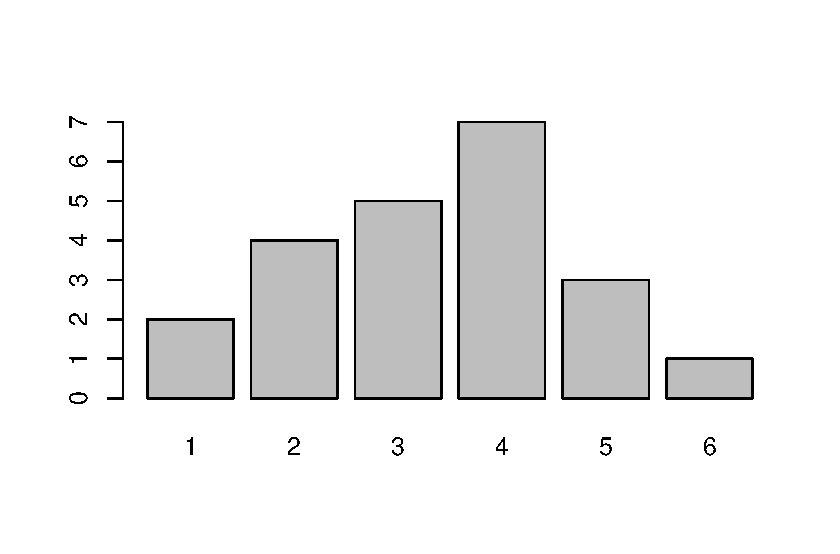
\includegraphics[width=0.9\linewidth]{Wahrscheinlichkeit-8_files/figure-latex/SaeulendiagrammBeispiel-1} \end{center}

Schließlich lässt sie sich von ihrem Rechner noch ein \textbf{Kreisdiagramm} erstellen, um eine bildlichere Vorstellung von der relativen Häufigkeit der Noten zu bekommen.

Beim Kreisdiagramm werden Anteile durch passende Winkel am Mittelpunkt des Kreises dargestellt. Der Vollkreis hat 360°. Einer relativen Häufigkeit von \(1\%\) entspricht also ein Kreissektor mit einem Mittelpunktswinkel von \(360° \cdot {1 \over 100} = 3,6°\). Einer relativen Häufigkeit von \(30\%\) entspricht damit ein Kreissektor mit einem Mittelpunktswinkel von \(30 \cdot 3,6° = 108°\)

\begin{center}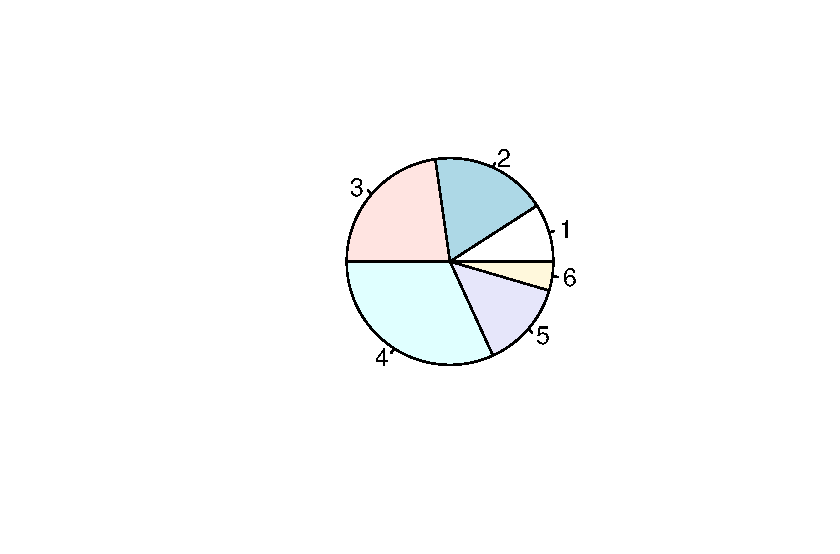
\includegraphics[width=0.9\linewidth]{Wahrscheinlichkeit-8_files/figure-latex/KreisdiagrammBeispiel-1} \end{center}

\hypertarget{section-15}{%
\subsubsection*{}\label{section-15}}
\addcontentsline{toc}{subsubsection}{}

\hypertarget{aufgabe-1-2}{%
\subsubsection*{Aufgabe 1}\label{aufgabe-1-2}}
\addcontentsline{toc}{subsubsection}{Aufgabe 1}

In einer Mathearbeit gab es folgende Noten:

Noten

Erstelle ein Säulen- und ein Kreisdiagramm für die Verteilung der Noten. Du kannst diese Aufgabe per Hand oder mit dem Computer lösen.

Tipp

Für das Kreisdiagramm musst du die relativen Häufigkeiten berechnen.

\hypertarget{section-16}{%
\subsubsection*{}\label{section-16}}
\addcontentsline{toc}{subsubsection}{}

Lösung

\begin{center}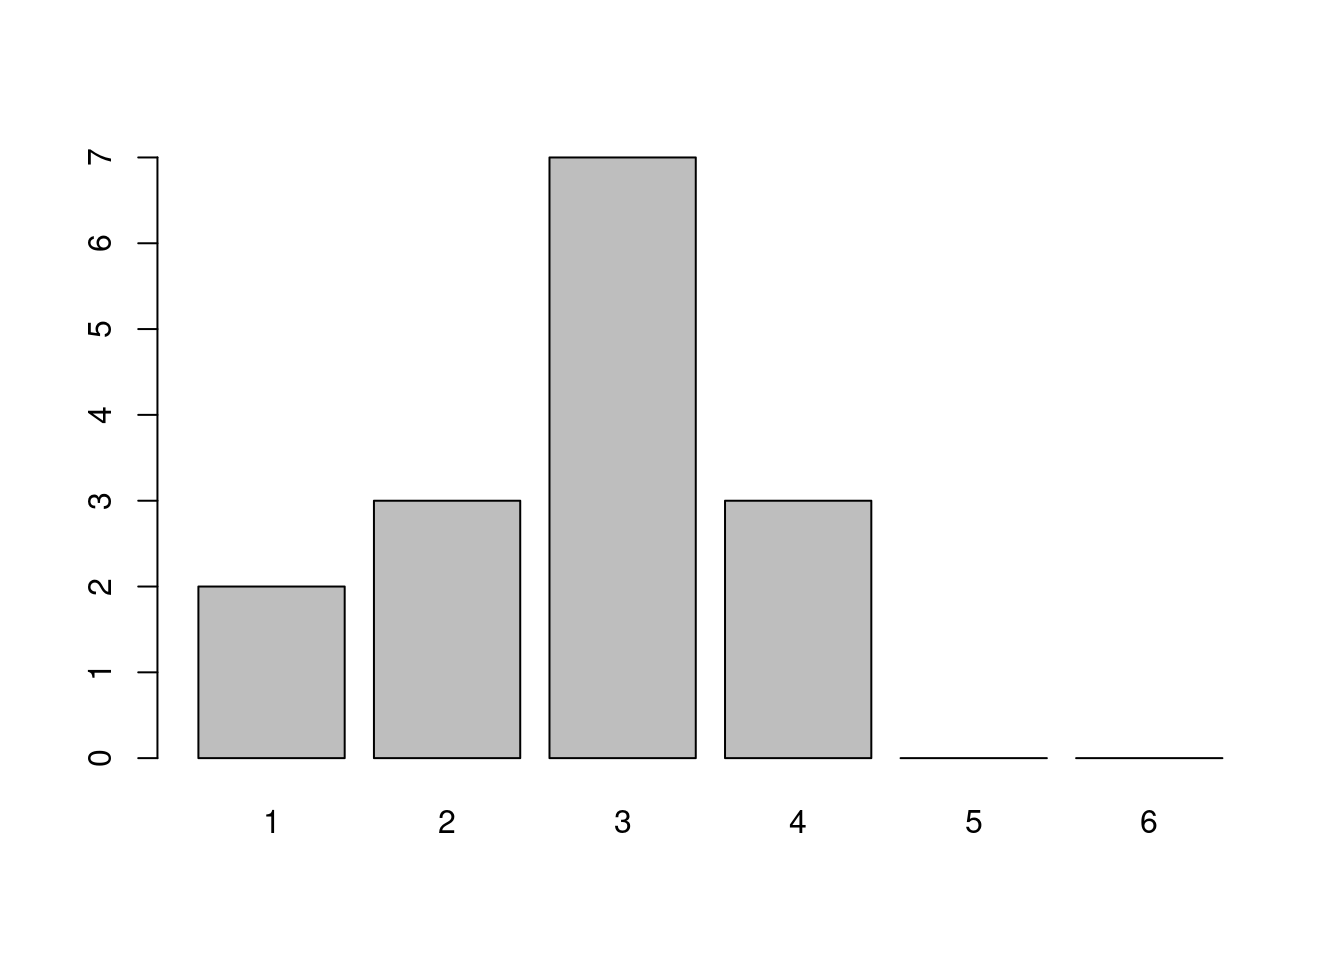
\includegraphics[width=0.9\linewidth]{Wahrscheinlichkeit-8_files/figure-latex/Aufgabe2.2.1-1} \end{center}

\begin{center}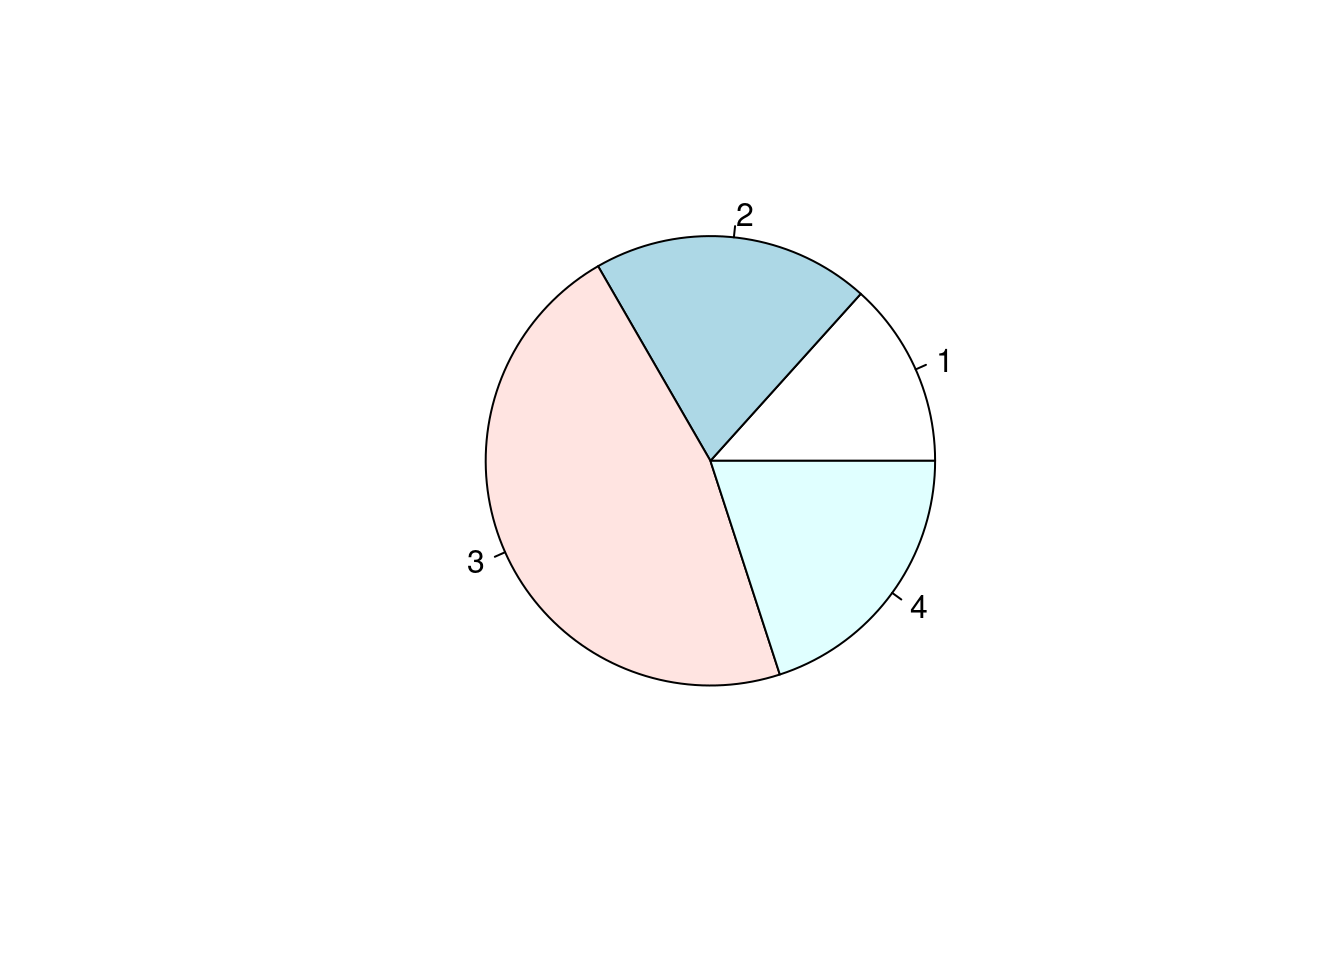
\includegraphics[width=0.9\linewidth]{Wahrscheinlichkeit-8_files/figure-latex/Aufgabe2.2.1-2} \end{center}

Für die Mittelpunktswinkel gilt hierbei:

\begin{longtable}[]{@{}lllll@{}}
\toprule
\begin{minipage}[b]{(\columnwidth - 4\tabcolsep) * \real{0.61}}\raggedright
Note\strut
\end{minipage} & \begin{minipage}[b]{(\columnwidth - 4\tabcolsep) * \real{0.10}}\raggedright
1\strut
\end{minipage} & \begin{minipage}[b]{(\columnwidth - 4\tabcolsep) * \real{0.10}}\raggedright
2\strut
\end{minipage} & \begin{minipage}[b]{(\columnwidth - 4\tabcolsep) * \real{0.10}}\raggedright
3\strut
\end{minipage} & \begin{minipage}[b]{(\columnwidth - 4\tabcolsep) * \real{0.10}}\raggedright
4\strut
\end{minipage}\tabularnewline
\midrule
\endhead
\begin{minipage}[t]{(\columnwidth - 4\tabcolsep) * \real{0.61}}\raggedright
Anzahl\strut
\end{minipage} & \begin{minipage}[t]{(\columnwidth - 4\tabcolsep) * \real{0.10}}\raggedright
\(\quad\quad\quad 2\)\strut
\end{minipage} & \begin{minipage}[t]{(\columnwidth - 4\tabcolsep) * \real{0.10}}\raggedright
\(\quad\quad\quad 3\)\strut
\end{minipage} & \begin{minipage}[t]{(\columnwidth - 4\tabcolsep) * \real{0.10}}\raggedright
\(\quad\quad\quad 7\)\strut
\end{minipage} & \begin{minipage}[t]{(\columnwidth - 4\tabcolsep) * \real{0.10}}\raggedright
\(\quad\quad\quad 3\)\strut
\end{minipage}\tabularnewline
\begin{minipage}[t]{(\columnwidth - 4\tabcolsep) * \real{0.61}}\raggedright
Winkel\strut
\end{minipage} & \begin{minipage}[t]{(\columnwidth - 4\tabcolsep) * \real{0.10}}\raggedright
\({2\over 15}\cdot 360°=48°\)\strut
\end{minipage} & \begin{minipage}[t]{(\columnwidth - 4\tabcolsep) * \real{0.10}}\raggedright
\({3\over 15}\cdot 360°=72°\)\strut
\end{minipage} & \begin{minipage}[t]{(\columnwidth - 4\tabcolsep) * \real{0.10}}\raggedright
\({7\over 15}\cdot 360°=168°\)\strut
\end{minipage} & \begin{minipage}[t]{(\columnwidth - 4\tabcolsep) * \real{0.10}}\raggedright
\({3\over 15}\cdot 360°=72°\)\strut
\end{minipage}\tabularnewline
\bottomrule
\end{longtable}

\hypertarget{section-17}{%
\subsubsection*{}\label{section-17}}
\addcontentsline{toc}{subsubsection}{}

\hypertarget{aufgabe-2-2}{%
\subsubsection*{Aufgabe 2}\label{aufgabe-2-2}}
\addcontentsline{toc}{subsubsection}{Aufgabe 2}

Bei einer Umfrage unter echten Kerlen ergab sich, dass sich \(80\%\) für Fußball interessieren, \(10\%\) gerne Motorrad fahren, \(10\%\) schnelle Autos lieben, sich \(5\%\) für Fußball und schnelle Autos interessieren und \(3\%\) Fußball und ihr Motorrad lieben.

Die Aufgabe lautet: Stelle diesen Sachverhalt in einem Kreisdiagramm dar.

Anton zeichnet sofort los. Doch schon nach den ersten drei Angaben ist der Kreis ``voll''. Er jammert. Seine kleine Schwester sieht sich seinen Kreis an. Ziemlich schnell hat sie entdeckt, wie man das Problem lösen kann. Dazu muss sie nicht einmal einen neuen Kreis zeichnen.

Was tut sie?

\hypertarget{section-18}{%
\subsubsection*{}\label{section-18}}
\addcontentsline{toc}{subsubsection}{}

Lösung

Diejenigen, die 2 Hobbies haben, sind bei den Einzelhobbies bereits mit erfasst. Deshalb müssen sich die Bereiche im Kreisdiagramm, die beide Hobbies betreffen, überschneiden.

\begin{center}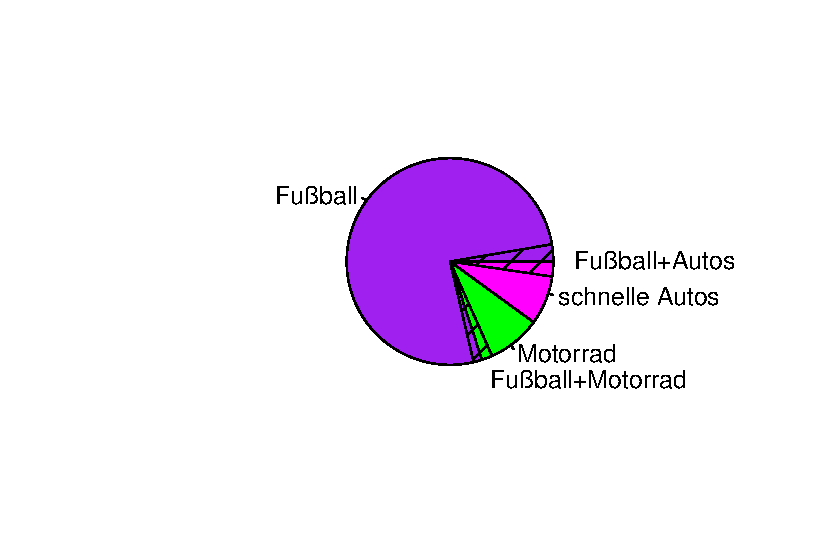
\includegraphics[width=0.9\linewidth]{Wahrscheinlichkeit-8_files/figure-latex/Aufgabe2.2.2-1} \end{center}

Grundsätzlich ist Antons Feststellung, dass der Kreis bereits nach den ersten drei Angaben ``voll'' ist, natürlich berechtigt, denn:

80\% Fußball + 10\% Motorrad + 10\% schnelle Autos = 100\% (und damit der Vollkreis)

Die beiden weiteren Kategorien kommen jedoch nicht noch zusätzlich dazu, sondern müssen in die bestehenden Kreissektoren einbeschrieben werden. Das erledigt die Schwester ganz geschickt mit Hilfe der gestrichelten Kreissektoren.

\hypertarget{section-19}{%
\subsubsection*{}\label{section-19}}
\addcontentsline{toc}{subsubsection}{}

\hypertarget{section-20}{%
\subsubsection*{}\label{section-20}}
\addcontentsline{toc}{subsubsection}{}

\hypertarget{das-arithmetische-mittel-die-spannweite-und-den-median-angeben}{%
\subsection*{Das arithmetische Mittel, die Spannweite und den Median angeben}\label{das-arithmetische-mittel-die-spannweite-und-den-median-angeben}}
\addcontentsline{toc}{subsection}{Das arithmetische Mittel, die Spannweite und den Median angeben}

Um kurze und prägnante (oft auch zu kurze!) Aussagen mit Hilfe der erhobenen Daten treffen zu können, bedient man sich der statistischen \textbf{Kennwerte}. Auch von diesen kennst du schon einige.

Das \textbf{arithmetische Mittel} beispielsweise ist Bestandteil des Alltags: Wenn wir vom ``Durchschnitt'' sprechen, meinen wir meist arithmetische Mittelwerte. Du erwartest ihn vermutlich auch als Angabe unter einer Klassenarbeit.

Das \textbf{arithmetische Mittel} berechnet man als \textbf{die Summe aller Werte durch die Anzahl der Werte}. Sehen wir uns als Beispiel die Fehleranzahl von 5 Grundschüler:innen in einem Diktat an.

\begin{longtable}[]{@{}ll@{}}
\toprule
& Anzahl der Fehler\tabularnewline
\midrule
\endhead
Anna & \(\quad\quad\quad 0\)\tabularnewline
Barbara & \(\quad\quad\quad 2\)\tabularnewline
Claire & \(\quad\quad\quad 4\)\tabularnewline
Dennis & \(\quad\quad\quad 3\)\tabularnewline
Enno & \(\quad\quad\quad 5\)\tabularnewline
\bottomrule
\end{longtable}

Das \textbf{arithmetische Mittel} ergibt sich also hier wie folgt:
\[\bar{x} = \frac{0+2+4+3+5}{5} = \frac{14}{5} =2,8\]

Das \textbf{arithmetische Mittel} hat allerdings einen kleinen Schwachpunkt. Es lässt sich - wie man sagt - von Ausreißern beeinflussen. Was das heißt, erkennt man ganz gut in dem Fall, in dem der arme Enno nicht ein einziges Wort richtig geschrieben hat\ldots{}

\begin{longtable}[]{@{}ll@{}}
\toprule
& Anzahl der Fehler\tabularnewline
\midrule
\endhead
Anna & \(\quad\quad\quad 0\)\tabularnewline
Barbara & \(\quad\quad\quad 2\)\tabularnewline
Claire & \(\quad\quad\quad 4\)\tabularnewline
Dennis & \(\quad\quad\quad 3\)\tabularnewline
Enno & \(\quad\quad\quad 131\)\tabularnewline
\bottomrule
\end{longtable}

Wenn der Grundschullehrer nun in einer Konferenz besorgt mitteilen würde, dass die Kinder im Diktat im Durchschnitt 28 Fehler machen, wäre dies sicher keine angemessene Aussage über die tatsächliche Leistung der Schüler:innen. Während Anna, Barbara, Claire und Dennis viel zu schlecht dastünden, käme Enno wiederum viel zu gut weg.

Diesen Nachteil hat der \textbf{Median} nicht (er hat andere). Der \textbf{Median} ist der Wert in der Mitte einer Rangliste. Hat die Rangliste eine ungerade Anzahl von Werten, so ist der mittlere Wert der \textbf{Median}. Hat die Rangliste eine gerade Anzahl von Werten, so bildet man den Mittelwert der beiden Werte in der Mitte.

Was heißt das?

Zunächst muss man also die Urliste der Größe nach sortieren. Für die fünf Grundschüler:innen erhält man dann je nach Szenarion
\[0;\; 2;\; \color{red}{3};\; 4;\; 5\]
oder
\[0;\; 2;\; \color{red}{3};\; 4;\; 131\]
Als Median erhält man also in beiden Fällen den Wert 3.

Und ja: Mehr muss man nicht tun. Man sortiert alle Werte der Größe nach und ermittelt den mittleren Wert.

Hätte nun auch noch Fritz am Diktat teilgenommen und ebenfalls 0 Fehler geschrieben, so sähe die Liste also wie folgt aus:
\[0;\;0;\; \color{red}{2};\; \color{red}{3};\; 4;\; 131\]
Der \textbf{Median} ist in diesem Fall definiert, als der Mittelwert aus den beiden mittleren Werten. In obigem Beispiel also \(\frac{2+3}{2}=2,5\)

Das \textbf{arithmetische Mittel} und der \textbf{Median} geben also Auskunft über den Durchschnitt. Der Durchschnitt alleine ist allerdings gar nicht unbedingt aussagekräftig.

Frau D. hat in zwei Parallelklassen eine Mathearbeit schreiben lassen. Wie es der Teufel will, kann sie in beiden Fällen stolz auf einen Durchschnitt von \(3,0\) blicken\ldots{}

Dass dies aber keineswegs bedeutet, dass die Klassenarbeiten gleich ausgefallen sein müssen, zeigt ein kurzer Blick auf die Notenverteilungen\ldots{}

Bei der Klasse 8x scheint es sich um eine sehr homogene Lerngruppe zu handeln:

\begin{center}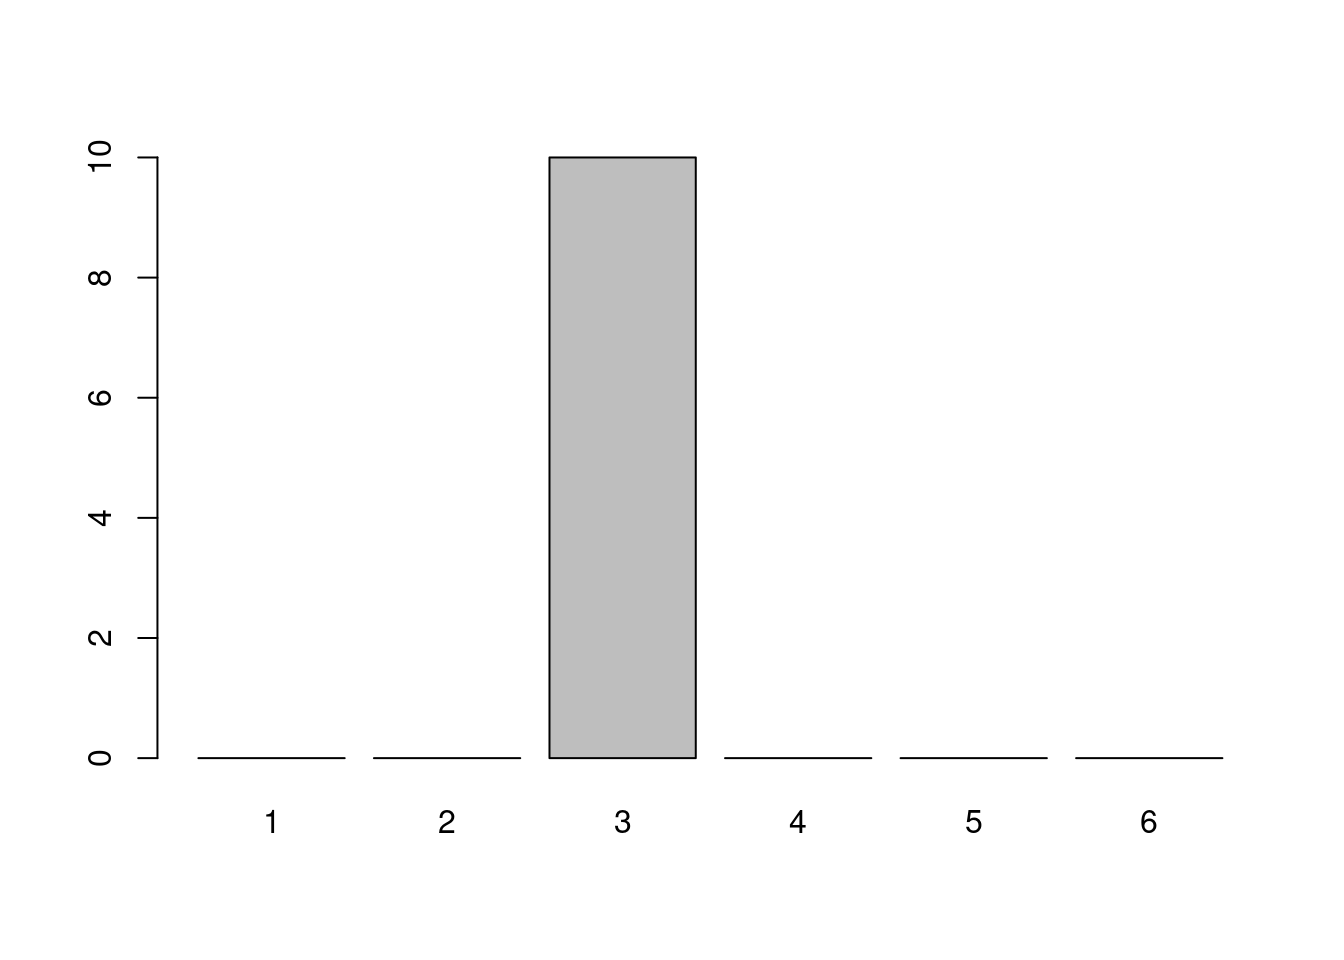
\includegraphics[width=0.9\linewidth]{Wahrscheinlichkeit-8_files/figure-latex/Notenverteilung1-1} \end{center}

Die Klasse 8y dagegen besticht durch ihre große \textbf{Spannweite}

\begin{center}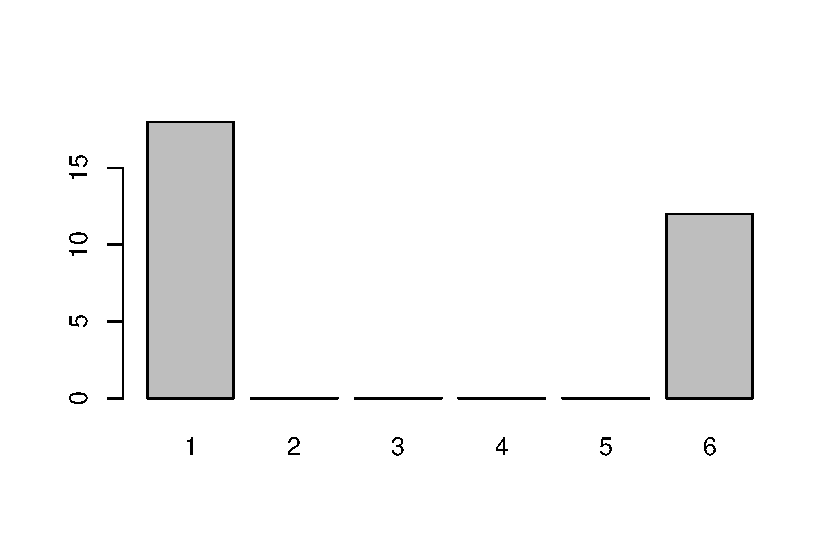
\includegraphics[width=0.9\linewidth]{Wahrscheinlichkeit-8_files/figure-latex/Notenverteilung2-1} \end{center}

Unter der \textbf{Spannweite} versteht man die Differenz aus dem größten und kleinsten Wert. Im Fall der Klasse 8x ist die Spannweite \(3-3=0\). Für die Klasse 8y ist sie \(6-1=5\). Wie auch bei der Berechnung des Mittelwerts kann ein Ausreißer für eine große Spannweite sorgen.

Um erhobene Daten kurz und prägnant zu beschreiben, ist es sinnvoll, neben der Angabe eines durchschnittlichen Wertes (Median oder Mittelwert), auch anzugeben, welche \textbf{Spannweite} die Daten haben.

\hypertarget{section-21}{%
\subsubsection*{}\label{section-21}}
\addcontentsline{toc}{subsubsection}{}

\hypertarget{aufgabe-1-3}{%
\subsubsection*{Aufgabe 1}\label{aufgabe-1-3}}
\addcontentsline{toc}{subsubsection}{Aufgabe 1}

In einer Mathearbeit gab es folgende Noten:

Noten

Gib das arithmetische Mittel, die Spannweite und den Median an.

\hypertarget{section-22}{%
\subsubsection*{}\label{section-22}}
\addcontentsline{toc}{subsubsection}{}

Lösung

Für das arithmetische Mittel gilt:

\[\bar{x}= \frac{1+3+3+2+2+3+3+4+2+1+3+4+4+3+3}{15} = \frac{41}{15} \approx 2,7\]

Die Spannweite ist \(4-1=3\).

Um den Median ermitteln zu können, sortiert man die Urliste zunächst und liest dann den mittleren Wert ab.

\[1\;, 1\;, 2\;, 2\;, 2\;, 3\;, 3\;, \color{red}{3}\;, 3\;, 3\;, 3\;, 3\;, 4\;, 4\;, 4\; \]

Der Median hat also den Wert 3.

\hypertarget{section-23}{%
\subsubsection*{}\label{section-23}}
\addcontentsline{toc}{subsubsection}{}

\hypertarget{aufgabe-2-3}{%
\subsubsection*{Aufgabe 2}\label{aufgabe-2-3}}
\addcontentsline{toc}{subsubsection}{Aufgabe 2}

Die Klasse 8x besteht aus 24 Schüler:innen. Das Kreisdiagramm enthält Informationen über das Alter der Schüler:innen.

\begin{center}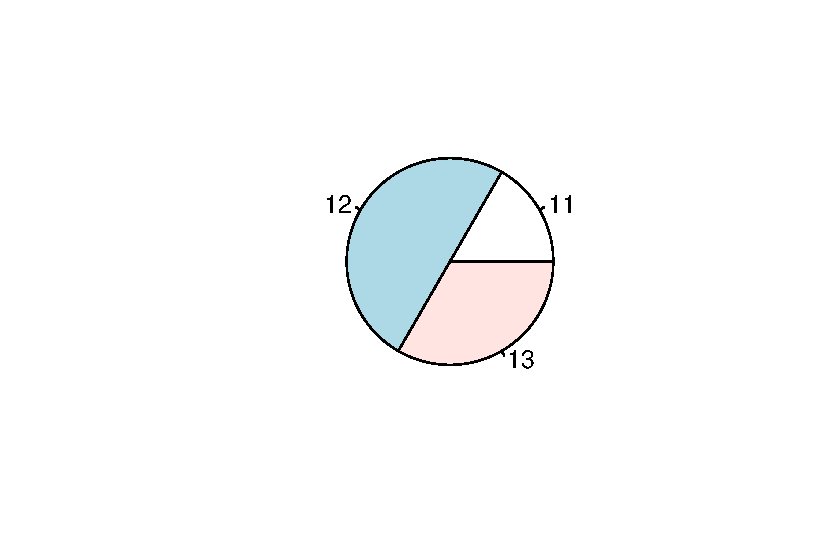
\includegraphics[width=0.9\linewidth]{Wahrscheinlichkeit-8_files/figure-latex/Aufgabe2.2.3-1} \end{center}

\begin{enumerate}
\def\labelenumi{\alph{enumi})}
\tightlist
\item
  Gib das durchschnittliche Alter an.
\end{enumerate}

\hypertarget{section-24}{%
\subsubsection*{}\label{section-24}}
\addcontentsline{toc}{subsubsection}{}

Lösung

Dem Kreisdiagramm entnimmt man, dass es 12 Schüler:innen (\(1\over 2\)) im Alter von 12 Jahren gibt, 4 Schüler:innen (\(1 \over 6\)) sind 11 Jahre alt und 8 Schüler:innen (\({2 \over 6} = \frac{1}{3}\)) sind 13 Jahre alt.

Folglich erhält man folgendes Durchschnittsalter:

\[\bar{x}= \frac{4 \cdot 11 + 12 \cdot 12 + 8 \cdot 13}{24} = 12\frac{1}{6}\]

Die Schüler:innen sind also durchschnittlich 12 Jahre und 2 Monate alt.

\hypertarget{section-25}{%
\subsubsection*{}\label{section-25}}
\addcontentsline{toc}{subsubsection}{}

\begin{enumerate}
\def\labelenumi{\alph{enumi})}
\setcounter{enumi}{1}
\tightlist
\item
  Ermittle, wie sich der Altersdurchschnitt ändert, wenn zwei 11-jährige Schüler die 8x verlassen und eine 14-jährige Schülerin neu in die Klasse kommt.
\end{enumerate}

\hypertarget{section-26}{%
\subsubsection*{}\label{section-26}}
\addcontentsline{toc}{subsubsection}{}

Lösung

Wenn zwei 11-jährige Schüler die 8x verlassen und eine 14-jährige Schülerin neu in die Klasse kommt, ändert sich die Altersverteilung wie folgt:

Neben der neuen einen 14-jährigen Schülerin gibt es immer noch 12 12-jährige Schüler:innen und 8 13-jährige Schüler:innen, aber nur noch 2 11-jährige Schüler:innen. Insgesamt besteht die Klasse nun aus 23 Schüler:innen.

Folglich erhält man nun folgendes Durchschnittsalter:

\[\bar{x}= \frac{2 \cdot 11 + 12 \cdot 12 + 8 \cdot 13 + 14}{23} = 12\frac{8}{23} \approx 12, 35\]

Die Schüler:innen sind also durchschnittlich 12 Jahre und etwas mehr als 4 Monate alt.

\hypertarget{section-27}{%
\subsubsection*{}\label{section-27}}
\addcontentsline{toc}{subsubsection}{}

\hypertarget{section-28}{%
\subsubsection*{}\label{section-28}}
\addcontentsline{toc}{subsubsection}{}

\hypertarget{box-plots-interpretieren-und-erstellen}{%
\subsection*{Box-Plots interpretieren und erstellen}\label{box-plots-interpretieren-und-erstellen}}
\addcontentsline{toc}{subsection}{Box-Plots interpretieren und erstellen}

Neben der Möglichkeit erhobene Daten in Form einer \textbf{Tabelle}, eines \textbf{Säulen-} oder eines \textbf{Kreisdiagramms} darzustellen, solltest in der 7. Klasse auch die Darstellung in Form eines \textbf{Boxplots} kennengelernt haben.

Ein Boxplot enthält sowohl Information über einen durchschnittlichen Wert, als auch darüber, welche Spannweite die Daten vorweisen. Daher ist er von allen Darstellungsformen, die dir bisher begegnet sind, die aussagekräftigste.

Anhand der ausgefallenen Mathearbeit soll er hier kurz wiederholt werden.

\begin{center}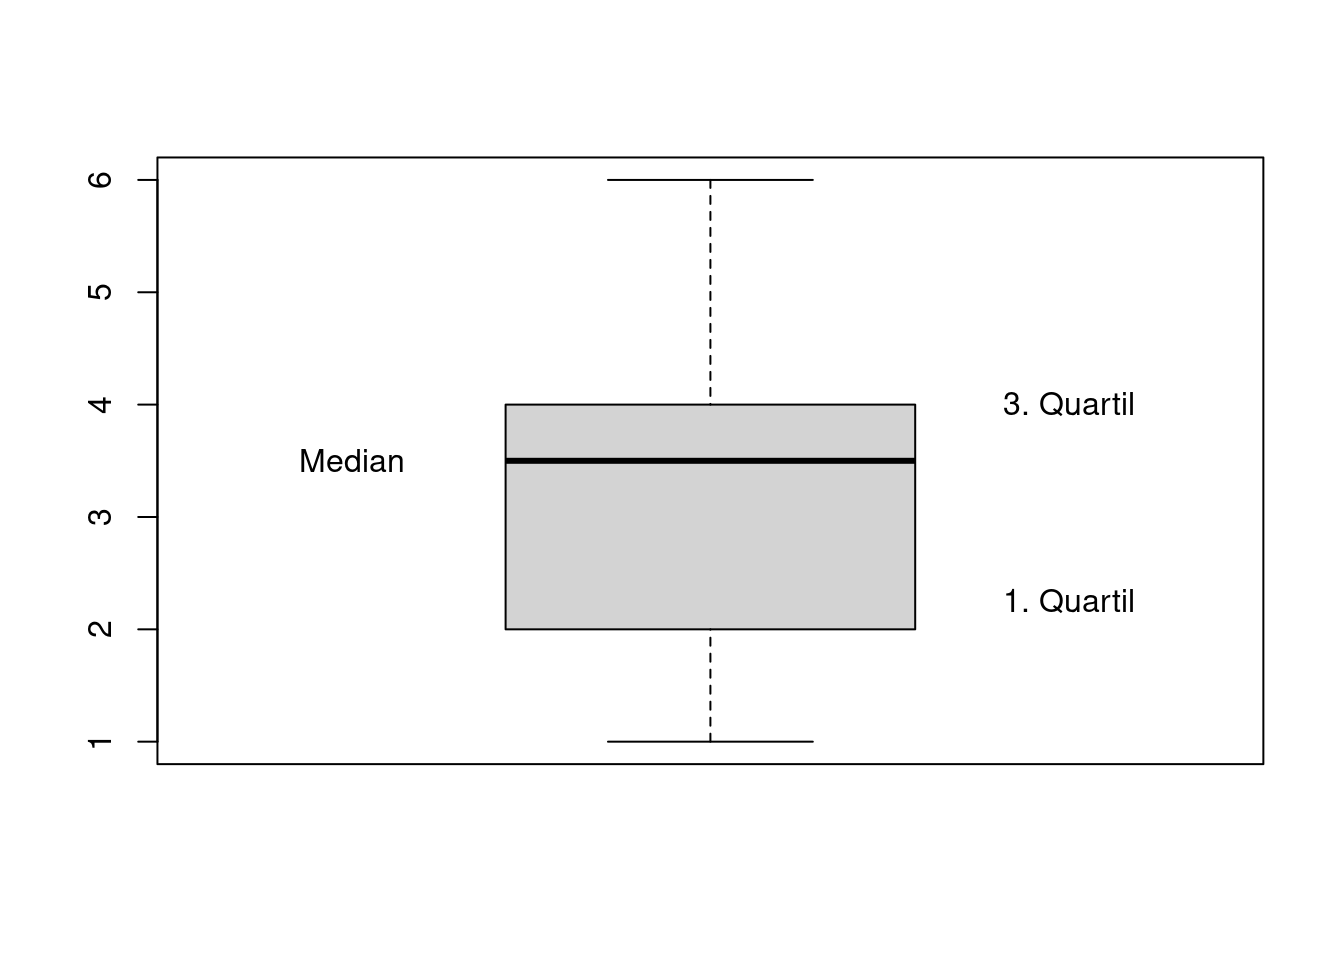
\includegraphics[width=0.9\linewidth]{Wahrscheinlichkeit-8_files/figure-latex/BoxplotBeispiel-1} \end{center}

Die Box wird dabei begrenzt durch das \textbf{1.} und \textbf{3. Quartil}. Das \textbf{1. Quartil} ist der mittlere Wert der unteren Datenhälfte, das \textbf{3. Quartil} ist der mittlere Wert der oberen Datenhälfte. Unterteilt wird die Box durch den \textbf{Median}.

Im Beispiel der Mathearbeit sind das folgende Werte:

\[1\;,1\;,2\;,2\;,2\;,\color{red}{2}\;,3\;,3\;,3\;,3\;,3\;,\color{red}{\frac{3+4}{2}},4\;,4\;,4\;,4\;,4\;,\color{red}{4}\;,4\;,5\;,5\;,5\;,6\]

Damit liegen \(50\%\) der Werte in der Box! Sie gibt also eine guten Eindruck davon, welche Werte oft vertreten waren. Gleichzeitig kann man an der Größe der Box auf einen Blick abschätzen wie groß die Spannweite sein könnte.

Die Querstriche am oberen und unteren Ende bezeichnet man als \textbf{Zäune}. In unseren Beispielen genügt es, für den unteren \textbf{Zaun} den kleinesten und für den oberen \textbf{Zaun} den größten Wert zu wählen.

\hypertarget{section-29}{%
\subsubsection*{}\label{section-29}}
\addcontentsline{toc}{subsubsection}{}

\hypertarget{aufgabe-1-4}{%
\subsubsection*{Aufgabe 1}\label{aufgabe-1-4}}
\addcontentsline{toc}{subsubsection}{Aufgabe 1}

Wie sieht ein Boxplot aus, wenn

\begin{enumerate}
\def\labelenumi{\alph{enumi})}
\tightlist
\item
  alle 30 Zahlen den Wert 3 besitzen (siehe Klasenarbeit der Klasse 8x)?
\end{enumerate}

\hypertarget{section-30}{%
\subsubsection*{}\label{section-30}}
\addcontentsline{toc}{subsubsection}{}

Lösung

\begin{center}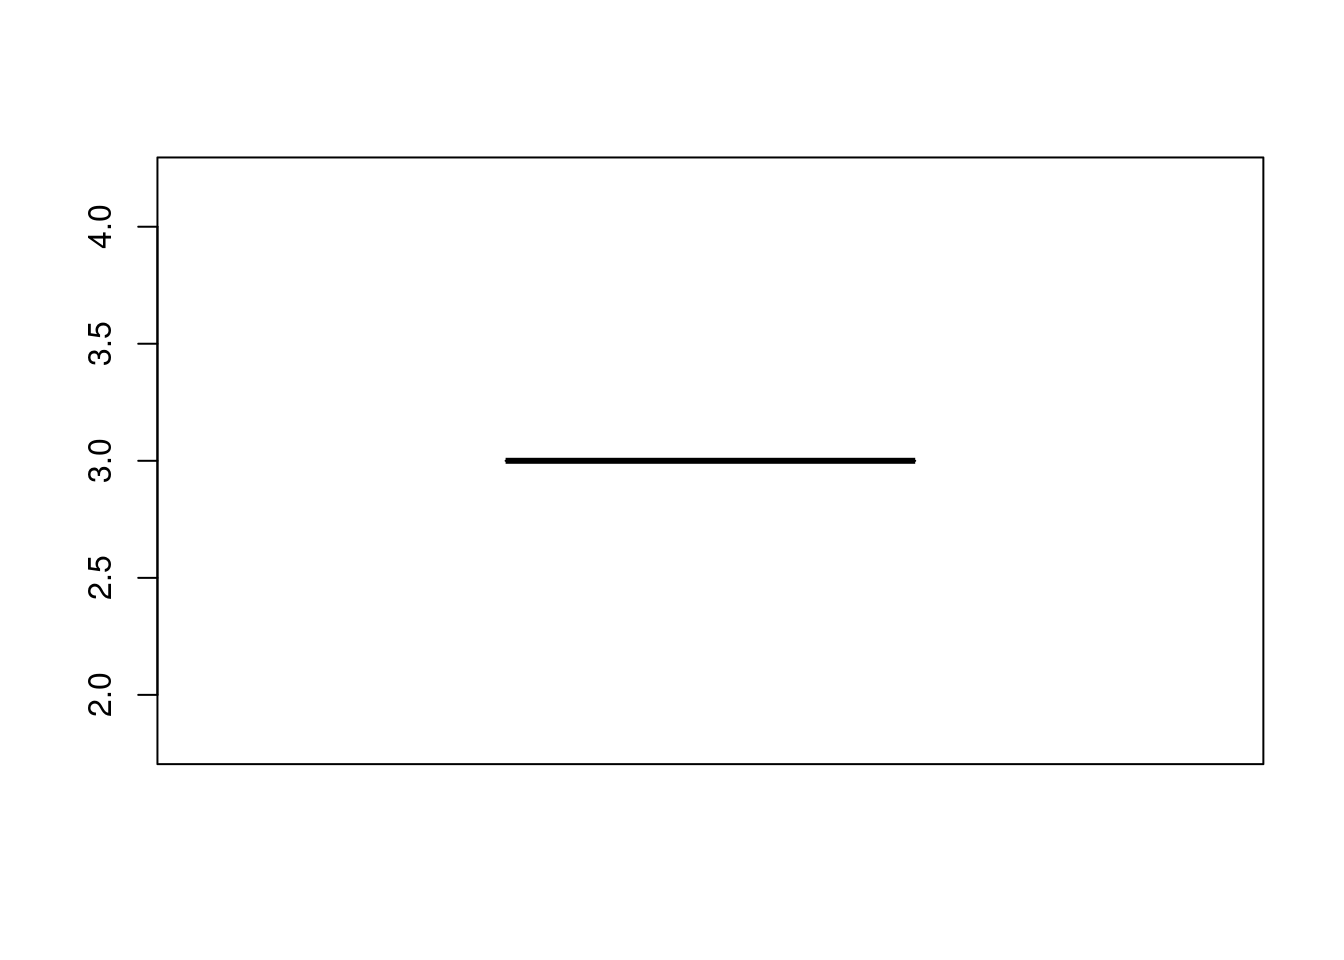
\includegraphics[width=0.9\linewidth]{Wahrscheinlichkeit-8_files/figure-latex/Aufgabe2.2.4-1} \end{center}

\hypertarget{section-31}{%
\subsubsection*{}\label{section-31}}
\addcontentsline{toc}{subsubsection}{}

\begin{enumerate}
\def\labelenumi{\alph{enumi})}
\setcounter{enumi}{1}
\tightlist
\item
  12 Zahlen den Wert 6 und 18 Zahlen den Wert 1 haben (siehe Klassenarbeit der Klasse 8y)?
\end{enumerate}

Lösung

\begin{center}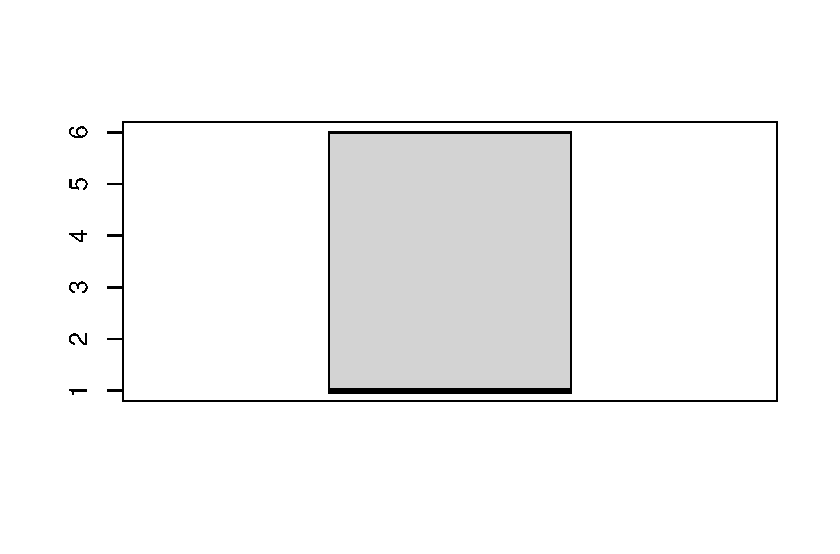
\includegraphics[width=0.9\linewidth]{Wahrscheinlichkeit-8_files/figure-latex/Aufgabe2.2.5-1} \end{center}

\hypertarget{section-32}{%
\subsubsection*{}\label{section-32}}
\addcontentsline{toc}{subsubsection}{}

\begin{enumerate}
\def\labelenumi{\alph{enumi})}
\setcounter{enumi}{2}
\tightlist
\item
  Wie könnte die Datenliste aussehen, wenn die Box des Boxplots die Länge 0 hat und der Abstand der beiden Zäune 10 sein soll?
\end{enumerate}

\hypertarget{section-33}{%
\subsubsection*{}\label{section-33}}
\addcontentsline{toc}{subsubsection}{}

Lösung

Die Datenliste könnte beispielsweise so aussehen:

0, 5, 5, 5, 5, 5, 5, 5, 5, 5, 5, 5, 10

\hypertarget{section-34}{%
\subsubsection*{}\label{section-34}}
\addcontentsline{toc}{subsubsection}{}

\hypertarget{aufgabe-2-4}{%
\subsubsection*{Aufgabe 2}\label{aufgabe-2-4}}
\addcontentsline{toc}{subsubsection}{Aufgabe 2}

Die folgende Liste zeigt, wie lange Hugo beim Würfeln jeweils auf die erste 6 warten musste.
\[1\;, 5\;, 11\;, 4\;, 15\;, 3\;, 7\;, 6\;, 1\;, 3\;, 1\;, 4\]

Stelle die Ergebnisse mit Hilfe eines Boxplots dar.

\hypertarget{section-35}{%
\subsubsection*{}\label{section-35}}
\addcontentsline{toc}{subsubsection}{}

Lösung

\begin{center}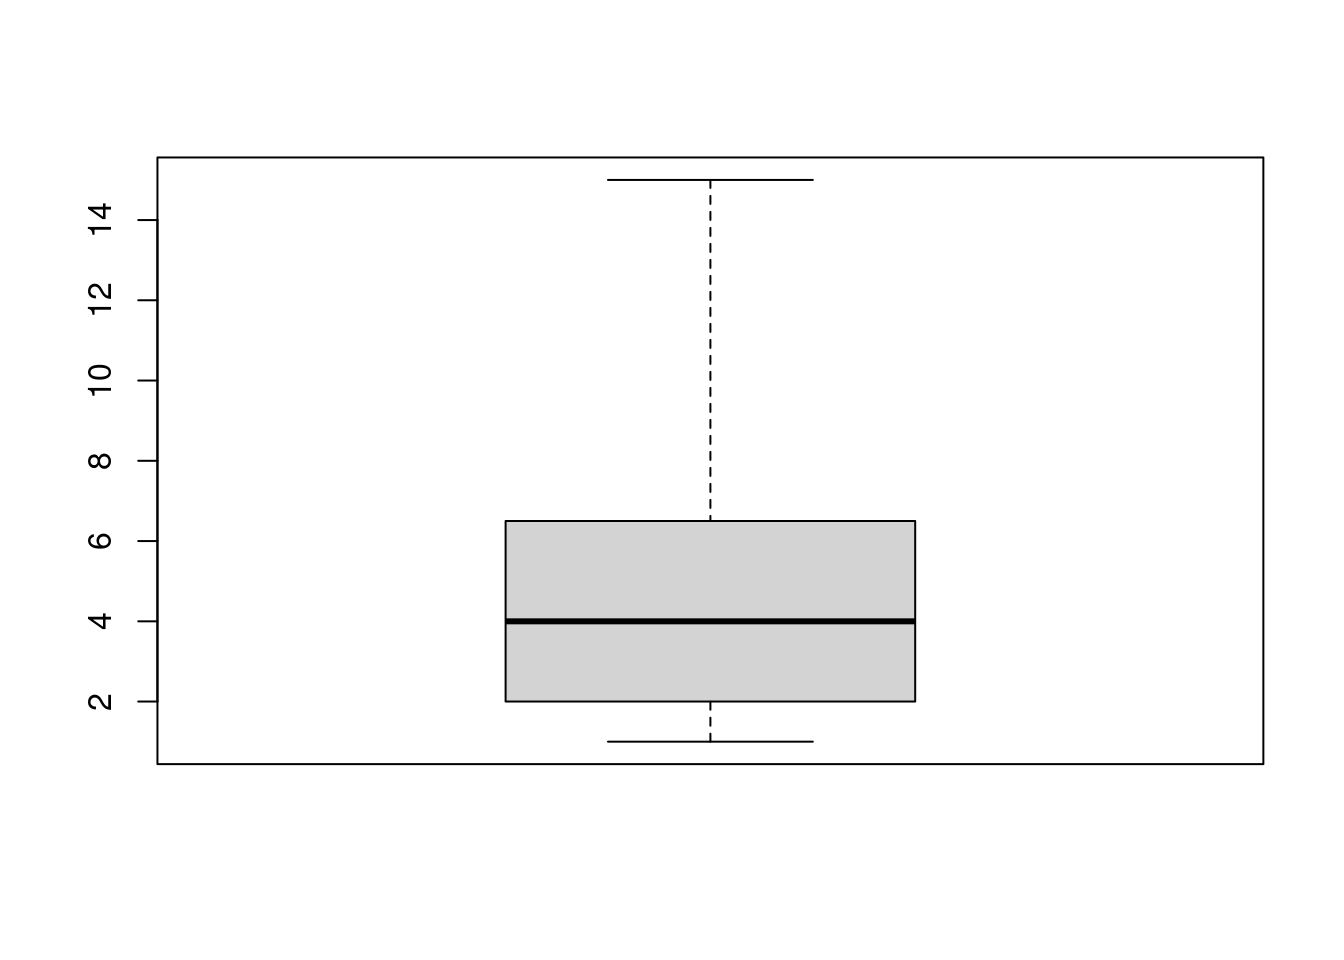
\includegraphics[width=0.9\linewidth]{Wahrscheinlichkeit-8_files/figure-latex/Aufgabe2.2.6-1} \end{center}

Der Median hat hierbei den Wert 4, das 1. Quartil hat den Wert 2 und das 3. Quartil hat den Wert 6,5.

\hypertarget{section-36}{%
\subsubsection*{}\label{section-36}}
\addcontentsline{toc}{subsubsection}{}

\hypertarget{aufgabe-3-1}{%
\subsubsection*{Aufgabe 3}\label{aufgabe-3-1}}
\addcontentsline{toc}{subsubsection}{Aufgabe 3}

Ordne zu. Welcher Boxplot gehört zu welchem Säulendiagramm?

A

\begin{center}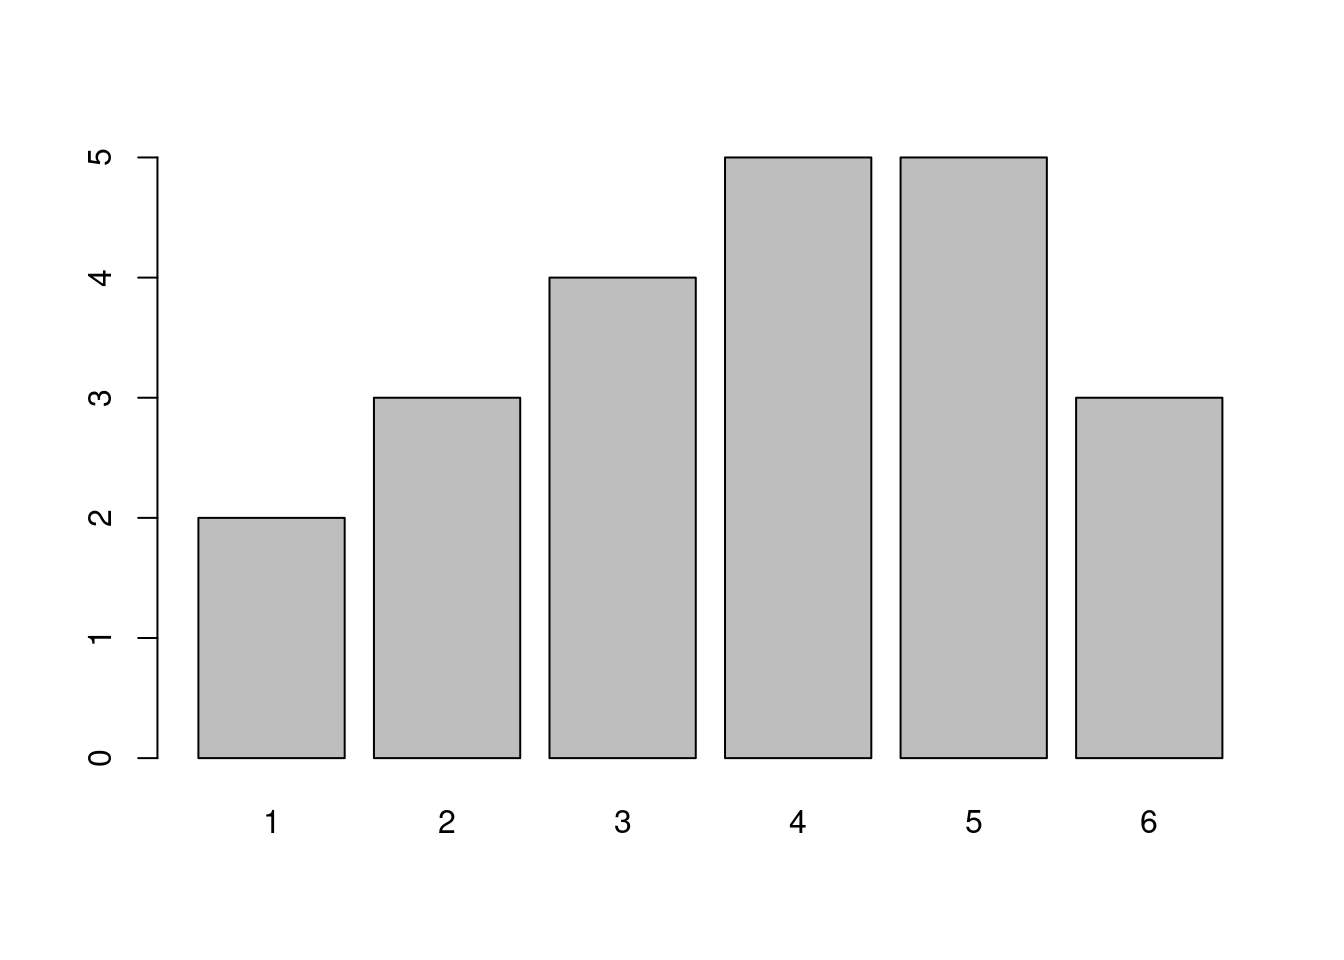
\includegraphics[width=0.9\linewidth]{Wahrscheinlichkeit-8_files/figure-latex/Aufgabe2.2.7-1} \end{center}

B

\begin{center}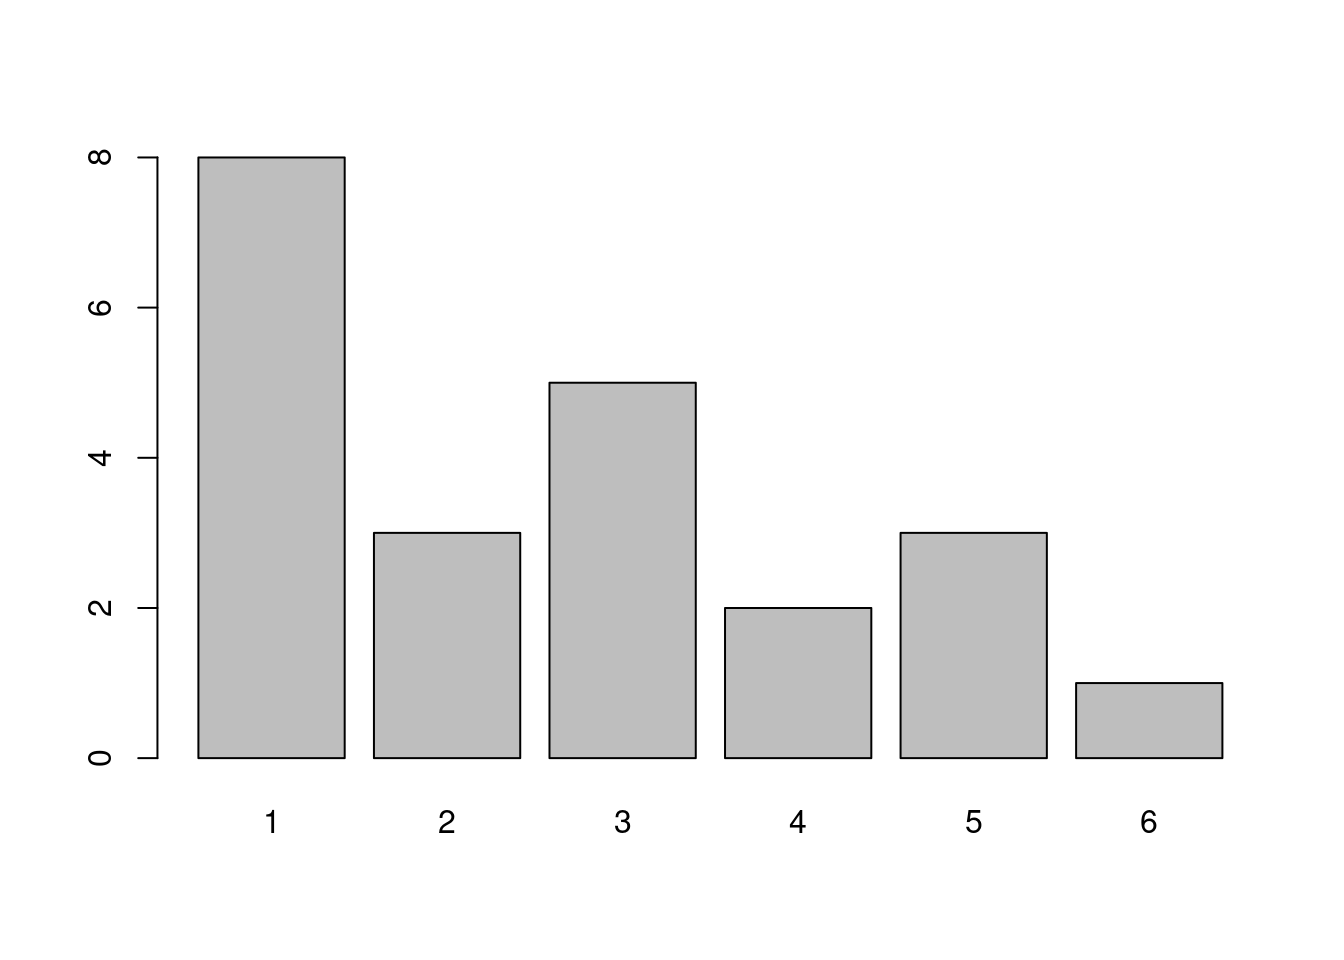
\includegraphics[width=0.9\linewidth]{Wahrscheinlichkeit-8_files/figure-latex/Aufgabe2.2.8-1} \end{center}

C

\begin{center}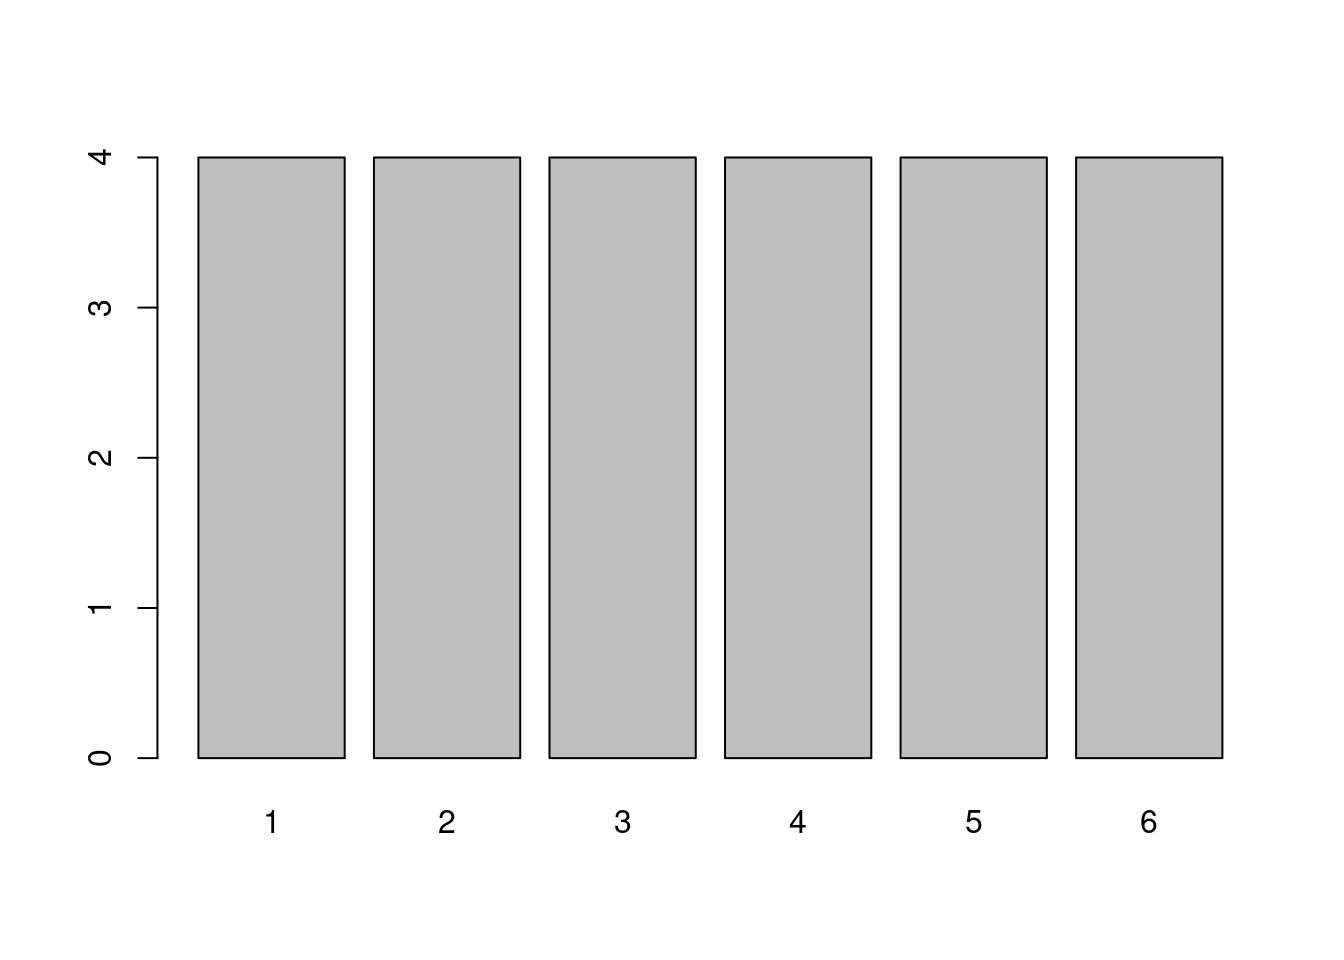
\includegraphics[width=0.9\linewidth]{Wahrscheinlichkeit-8_files/figure-latex/Aufgabe2.2.9-1} \end{center}

A

\begin{center}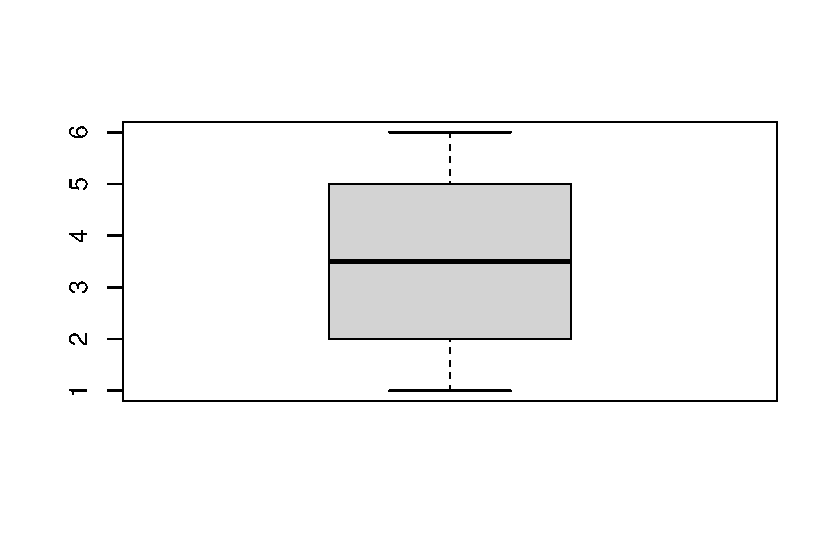
\includegraphics[width=0.9\linewidth]{Wahrscheinlichkeit-8_files/figure-latex/Aufgabe2.2.10-1} \end{center}

B

\begin{center}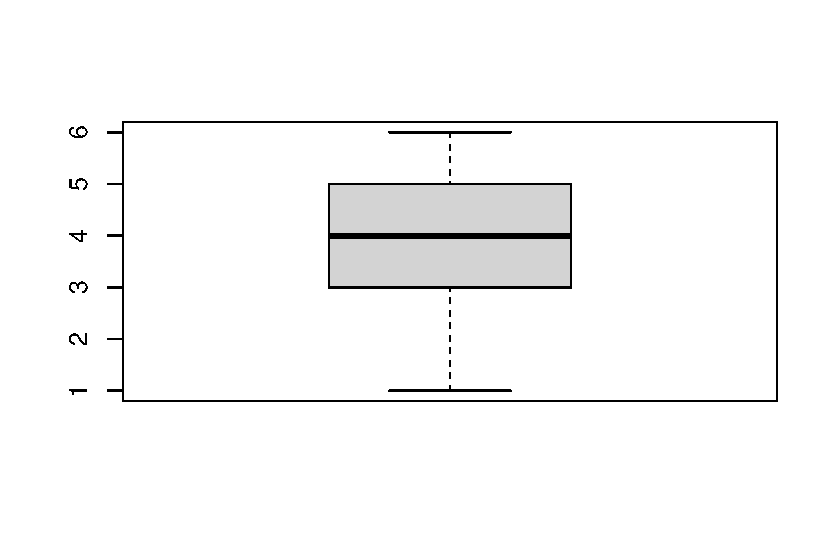
\includegraphics[width=0.9\linewidth]{Wahrscheinlichkeit-8_files/figure-latex/Aufgabe2.2.11-1} \end{center}

C

\begin{center}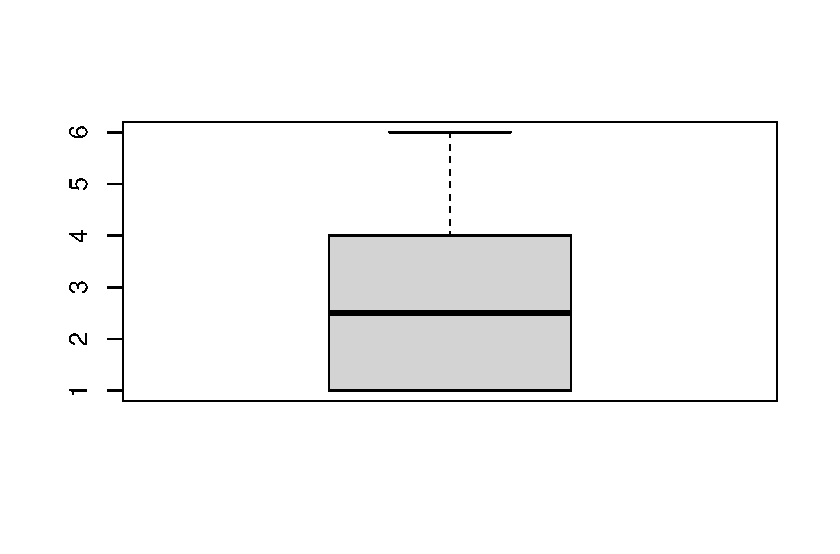
\includegraphics[width=0.9\linewidth]{Wahrscheinlichkeit-8_files/figure-latex/Aufgabe2.2.12-1} \end{center}

\hypertarget{section-37}{%
\subsubsection*{}\label{section-37}}
\addcontentsline{toc}{subsubsection}{}

Lösung

\begin{itemize}
\item
  Boxplot A gehört zu Säulendiagramm C.
\item
  Boxplot B gehört zu Säulendiagramm A.
\item
  Boxplot C gehört zu Säulendiagramm B.
\end{itemize}

\hypertarget{section-38}{%
\subsubsection*{}\label{section-38}}
\addcontentsline{toc}{subsubsection}{}

\hypertarget{wahrscheinlichkeit---da-war-doch-was}{%
\section{Wahrscheinlichkeit - da war doch was}\label{wahrscheinlichkeit---da-war-doch-was}}

Bevor der Begriff der \emph{Wahrscheinlichkeit} eingeführt wird, beschäftigen wir uns mit den Grundbausteinen der Wahrscheinlichkeitsrechnung, den sogenannten zufälligen Ereignissen.

\hypertarget{zufallsexperimente}{%
\subsection*{Zufallsexperimente}\label{zufallsexperimente}}
\addcontentsline{toc}{subsection}{Zufallsexperimente}

Bei der Durchführung vieler Experimente kann eines von mehreren möglichen Ergebnissen eintreten. Dabei sind zwar die verschiedenen Ergebnisse, die eintreten können bekannt, vor der Durchführung des Experiments weiß man jedoch nicht, welches Ergebnis tatsächlich eintreten wird. In solchen Fällen sagt man, das Ergebnis hängt vom Zufall ab. Deshalb nennt man derartige Experimente auch \emph{Zufallsexperimente}.

Ein Zufallsexperiment liegt vor, wenn folgende vier Bedingungen erfüllt sind:

\begin{itemize}
\item
  Ein Zufallsexperiment kann verschieden ausgehen.
\item
  Alle möglichen Ausgänge oder auch Ergebnisse des Experiments können vor dem Experiment angegeben werden.
\item
  Wie das Experiment ausgehen wird, lässt sich nicht mit Sicherheit voraussagen.
\item
  Das Experiment kann unter gleichen Bedingungen beliebig oft wiederholt werden.
\end{itemize}

Beispiele für Zufallsexperimente sind:

Würfeln, eine Münze werfen, Lotto spielen, einen Gegenstand blind aus einem Sack ziehen, die Körpergröße, das Gewicht oder auch den Blutdruck einer zufällig ausgewählten Person messen usw..

\hypertarget{section-39}{%
\subsubsection*{}\label{section-39}}
\addcontentsline{toc}{subsubsection}{}

\hypertarget{aufgabe-1-5}{%
\subsubsection*{Aufgabe 1}\label{aufgabe-1-5}}
\addcontentsline{toc}{subsubsection}{Aufgabe 1}

Ein Zufallsexperiment ist ein Vorgang, dessen Sudoku spielen gleichen beliebig oft Ausgang mehrere Würfel zu werfen Zufallsexperiment vorhersagen man nicht Sudoku spielen gleichen beliebig oft Ausgang mehrere Würfel zu werfen Zufallsexperiment vorhersagen kann. Bei einem Sudoku spielen gleichen beliebig oft Ausgang mehrere Würfel zu werfen Zufallsexperiment vorhersagen sollen Sudoku spielen gleichen beliebig oft Ausgang mehrere Würfel zu werfen Zufallsexperiment vorhersagen Ausgänge möglich sein und es soll Sudoku spielen gleichen beliebig oft Ausgang mehrere Würfel zu werfen Zufallsexperiment vorhersagen unter den Sudoku spielen gleichen beliebig oft Ausgang mehrere Würfel zu werfen Zufallsexperiment vorhersagen Bedingungen wiederholbar sein.

Eine Münze oder Sudoku spielen gleichen beliebig oft Ausgang mehrere Würfel zu werfen Zufallsexperiment vorhersagen zählen zu Zufallsexperimenten. Sudoku spielen gleichen beliebig oft Ausgang mehrere Würfel zu werfen Zufallsexperiment vorhersagen ist kein Zufallsexperiment, da kein Zufall im Spiel ist.

\hypertarget{section-40}{%
\subsubsection*{}\label{section-40}}
\addcontentsline{toc}{subsubsection}{}

\hypertarget{aufgabe-2-5}{%
\subsubsection*{Aufgabe 2}\label{aufgabe-2-5}}
\addcontentsline{toc}{subsubsection}{Aufgabe 2}

Entscheide, ob es sich um ein Zufallsexperiment handelt.

\begin{itemize}
\item
  Lose ziehen Ja, das ist ein Zufallsexperiment Nein, das ist kein Zufallsexperiment
\item
  Würfeln Ja, das ist ein Zufallsexperiment Nein, das ist kein Zufallsexperiment
\item
  Die Temperatur bestimmen, bei der Eis schmilzt Ja, das ist ein Zufallsexperiment Nein, das ist kein Zufallsexperiment
\item
  Blind eine Spielkarte aus einem Kartendeck ziehen Ja, das ist ein Zufallsexperiment Nein, das ist kein Zufallsexperiment
\item
  Die Innenwinkelsumme eines zufälligen Dreiecks bestimmen Ja, das ist ein Zufallsexperiment Nein, das ist kein Zufallsexperiment
\end{itemize}

\hypertarget{section-41}{%
\subsubsection*{}\label{section-41}}
\addcontentsline{toc}{subsubsection}{}

\hypertarget{section-42}{%
\subsubsection*{}\label{section-42}}
\addcontentsline{toc}{subsubsection}{}

\hypertarget{die-ergebnismenge-eines-einfachen-zufallsexperiments}{%
\subsection*{Die Ergebnismenge eines einfachen Zufallsexperiments}\label{die-ergebnismenge-eines-einfachen-zufallsexperiments}}
\addcontentsline{toc}{subsection}{Die Ergebnismenge eines einfachen Zufallsexperiments}

Die möglichen Ausgänge eines Zufallsexperiments werden als \textbf{Ergebnisse} bezeichnet. Die Menge der möglichen Ausgänge bezeichnet man als \textbf{Ergebnismenge}. Sie fasst alle Ausgänge eines Zufallexperiments zusammen.

Schreibweise: \(\Omega = \{a,\;b,\;c\}\)

Sprich: ``Die Ergebnismenge \emph{Omega} besteht aus den Ergebnissen a, b und c.''

Beispiele:

\begin{itemize}
\item
  Eine Münze werfen hat die Ergebnismenge: \(\Omega=\{Kopf,\; Zahl\}\)
\item
  Würfeln hat die Ergebnismenge: \(\Omega=\{1\;, 2,\; 3,\;4,\;5,\;6\}\)
\item
  An dem unten abgebildeten Glücksrad drehen hat die Ergebnismenge: \(\Omega=\{1\;, 2\;, 3\}\)
\end{itemize}

\hypertarget{section-43}{%
\subsubsection*{}\label{section-43}}
\addcontentsline{toc}{subsubsection}{}

\hypertarget{aufgabe-1-6}{%
\subsubsection*{Aufgabe 1}\label{aufgabe-1-6}}
\addcontentsline{toc}{subsubsection}{Aufgabe 1}

Notiere die Ergebnismengen für folgende Zufallsexperimente:

\begin{enumerate}
\def\labelenumi{\alph{enumi})}
\tightlist
\item
  Würfeln mit folgenden Würfeln
\end{enumerate}

\begin{enumerate}
\def\labelenumi{\alph{enumi})}
\setcounter{enumi}{1}
\tightlist
\item
  Man dreht folgende Glücksräder
\end{enumerate}

\begin{enumerate}
\def\labelenumi{\alph{enumi})}
\setcounter{enumi}{2}
\tightlist
\item
  Man würfelt zwei ``normale'' Würfel und bildet anschließend die Augensumme.
\end{enumerate}

\hypertarget{section-44}{%
\subsubsection*{}\label{section-44}}
\addcontentsline{toc}{subsubsection}{}

Lösung

\begin{enumerate}
\def\labelenumi{\alph{enumi})}
\tightlist
\item
  Würfel mit acht Seiten: \(\Omega =\{1,\;2,\;3,\;4,\;5,\;6,\;7,\;8\}\)
\end{enumerate}

Würfel mit zwanzig Seiten: \(\Omega =\{1,\;2,\;3,\;4,...,\;16,\;17,\;18,\;19,\;20\}\)

\begin{enumerate}
\def\labelenumi{\alph{enumi})}
\setcounter{enumi}{1}
\tightlist
\item
  Erstes Glücksrad: \(\Omega = \{rot,\;blau,\;gelb,\;gruen \}\)
\end{enumerate}

Zweites Glücksrad: \(\Omega = \{rot,\;orange/Hauptgewinn,\;gelb,\;gruen,\;hellblau,\;dunkelblau \}\)

\begin{enumerate}
\def\labelenumi{\alph{enumi})}
\setcounter{enumi}{2}
\tightlist
\item
  Die Augensumme bei einem Wurf mit zwei Würfeln: \(\Omega =\{2,\;3,\;4,\;5,\;6,\;7,\;8,\;9,\;10,\;11,\;12\}\)
\end{enumerate}

\hypertarget{section-45}{%
\subsubsection*{}\label{section-45}}
\addcontentsline{toc}{subsubsection}{}

\hypertarget{aufgabe-2-6}{%
\subsubsection*{Aufgabe 2}\label{aufgabe-2-6}}
\addcontentsline{toc}{subsubsection}{Aufgabe 2}

Beschreibe passende Zufallsexperimente für folgende Ergebnismengen.

\begin{enumerate}
\def\labelenumi{\alph{enumi})}
\tightlist
\item
  \(\Omega = \{weiß,\; schwarz,\; rot,\; blau \}\)
\end{enumerate}

Lösung

Man dreht ein Glücksrad, das vier Sektoren mit den Farben weiß, schwarz, rot und blau hat.

\hypertarget{section-46}{%
\subsubsection*{}\label{section-46}}
\addcontentsline{toc}{subsubsection}{}

\begin{enumerate}
\def\labelenumi{\alph{enumi})}
\setcounter{enumi}{1}
\tightlist
\item
  \(\Omega = \{Niete,\; kleiner\;Gewinn,\; mittlerer\;Gewinn,\; großer\;Gewinn \}\)
\end{enumerate}

Lösung

Man zieht ein Los aus einer Lostrommel, die Nieten, kleine, mittlere und große Gewinne enthält.

\hypertarget{section-47}{%
\subsubsection*{}\label{section-47}}
\addcontentsline{toc}{subsubsection}{}

\begin{enumerate}
\def\labelenumi{\alph{enumi})}
\setcounter{enumi}{2}
\tightlist
\item
  \(\Omega = \{Song1,\; Song2,\; Song3,\; Song4 \}\)
\end{enumerate}

Lösung

Man wählt ``zufällige Wiedergabe'' bei einer Playliste, die nur vier Songs enthält.

\hypertarget{section-48}{%
\subsubsection*{}\label{section-48}}
\addcontentsline{toc}{subsubsection}{}

\hypertarget{section-49}{%
\subsubsection*{}\label{section-49}}
\addcontentsline{toc}{subsubsection}{}

\hypertarget{zufuxe4llige-ereignisse}{%
\subsection*{Zufällige Ereignisse}\label{zufuxe4llige-ereignisse}}
\addcontentsline{toc}{subsection}{Zufällige Ereignisse}

Ein zufälliges Ereignis (oder einfach Ereignis) ist eine Teilmenge der Ergebnismenge. Ein Ereignis ist also ein möglicher Versuchsausgang eines Zufallsexperiments, der aus einem oder mehreren Ergebnissen besteht.

Mit anderen Worten: Mehrere Ergebnisse können zu einem \textbf{Ereignis} zusammengefasst werden.

Schreibweise: \(E=\{a\;,b\;,c\}\)

Beispiele:

\begin{itemize}
\tightlist
\item
  Das Würfeln einer geraden Zahl kann geschrieben werden als \(E=\{2,\;4,\;6\}\)
\end{itemize}

\begin{itemize}
\tightlist
\item
  Das Würfeln einer Zahl kleiner 3 kann geschrieben werden als \(E=\{1,\;2\}\)
\end{itemize}

Es gibt drei besondere Ereignisse:

\begin{itemize}
\item
  Das \textbf{Elementarereignis}: Es enthält \textbf{nur ein} Ergebnis. {[}Eine 1 würfeln oder ``Kopf'' werfen.{]}
\item
  Das \textbf{sichere Ereignis}: Es enthält \textbf{alle} möglichen Ergebnisse und tritt daher bei jeder Durchführung des Zufallsexperiments ein. {[}Eine 1, 2, 3, 4, 5 oder 6 würfeln. ``Kopf'' oder ``Zahl'' werfen.{]}
\end{itemize}

\begin{itemize}
\tightlist
\item
  Das \textbf{unmögliche Ereignis}: Es enthält \textbf{kein} Ergebnis. {[}Eine 8 würfeln oder ``Rand'' werfen.{]}
\end{itemize}

\hypertarget{section-50}{%
\subsubsection*{}\label{section-50}}
\addcontentsline{toc}{subsubsection}{}

\hypertarget{aufgabe-1-7}{%
\subsubsection*{Aufgabe 1}\label{aufgabe-1-7}}
\addcontentsline{toc}{subsubsection}{Aufgabe 1}

Du hast folgende Urne. In ihr sind verschieden farbige, nummerierte Kugeln.

Als Zufallsexperiment zieht man nun eine Kugel aus der Urne. Formuliere Ereignisse, die folgende Eigenschaften erfüllen.

\begin{enumerate}
\def\labelenumi{\alph{enumi})}
\tightlist
\item
  Die Ereignismenge umfasst 3 Ergebnisse.
\end{enumerate}

Lösung

Ereignis: Die Zahl auf der gezogenen Kugel ist durch 3 teilbar. Ereignismenge: \(E=\{3,\;6,\;9\}\)

\hypertarget{section-51}{%
\subsubsection*{}\label{section-51}}
\addcontentsline{toc}{subsubsection}{}

\begin{enumerate}
\def\labelenumi{\alph{enumi})}
\setcounter{enumi}{1}
\tightlist
\item
  Die Ereignismenge umfasst kein Ergebnis.
\end{enumerate}

Lösung

Ereignis: Es wird eine weiße Kugel gezogen. Ereignismenge: \(E=\{\quad\}\)

\hypertarget{section-52}{%
\subsubsection*{}\label{section-52}}
\addcontentsline{toc}{subsubsection}{}

\begin{enumerate}
\def\labelenumi{\alph{enumi})}
\setcounter{enumi}{2}
\tightlist
\item
  Die Ereignismenge umfasst 4 Ergebnisse.
\end{enumerate}

Lösung

Ereignis: Es wird eine Kugel gezogen, auf der eine Zahl steht, die kleiner ist als 5. Ereignismenge: \(E=\{1,\;2,\;3,\;4\}\)

\hypertarget{section-53}{%
\subsubsection*{}\label{section-53}}
\addcontentsline{toc}{subsubsection}{}

\begin{enumerate}
\def\labelenumi{\alph{enumi})}
\setcounter{enumi}{3}
\tightlist
\item
  Die Ereignismenge umfasst ein Ergebnis.
\end{enumerate}

Lösung

Ereignis: Die gelbe Kugel wird gezogen. Ereignismenge: \(E=\{10\}\)

\hypertarget{section-54}{%
\subsubsection*{}\label{section-54}}
\addcontentsline{toc}{subsubsection}{}

\begin{enumerate}
\def\labelenumi{\alph{enumi})}
\setcounter{enumi}{4}
\tightlist
\item
  Die Ereignismenge umfasst 6 Ergebnisse.
\end{enumerate}

Lösung

Ereignis: Es wird eine Kugel gezogen, auf der eine Zahl zwischen 1 und 6 steht. Ereignismenge: \(E=\{1,\;2,\;3,\;4,\;5,\;6\}\)

\hypertarget{section-55}{%
\subsubsection*{}\label{section-55}}
\addcontentsline{toc}{subsubsection}{}

\hypertarget{aufgabe-2-7}{%
\subsubsection*{Aufgabe 2}\label{aufgabe-2-7}}
\addcontentsline{toc}{subsubsection}{Aufgabe 2}

Schreibe die Ereignismengen zu folgenden Ereignissen auf.

\begin{enumerate}
\def\labelenumi{\alph{enumi})}
\tightlist
\item
  Bei einem Würfelwurf fällt eine ungerade Zahl.
\end{enumerate}

Lösung

Ereignismenge: \(E=\{1,\;3,\;5\}\)

\hypertarget{section-56}{%
\subsubsection*{}\label{section-56}}
\addcontentsline{toc}{subsubsection}{}

\begin{enumerate}
\def\labelenumi{\alph{enumi})}
\setcounter{enumi}{1}
\tightlist
\item
  Beim Roulett wird kein schwarzes und kein rotes Feld getroffen.
\end{enumerate}

Lösung

Ereignismenge: \(E=\{Null\}\) (Die Null ist ein grünes Feld.)

\hypertarget{section-57}{%
\subsubsection*{}\label{section-57}}
\addcontentsline{toc}{subsubsection}{}

\begin{enumerate}
\def\labelenumi{\alph{enumi})}
\setcounter{enumi}{2}
\tightlist
\item
  Alle möglichen Geburtstage im Monat Februar für die gilt, dass sie nach dem 29.2. stattfinden.
\end{enumerate}

Lösung

Ereignismenge: \(E=\{\quad\}\)

\hypertarget{section-58}{%
\subsubsection*{}\label{section-58}}
\addcontentsline{toc}{subsubsection}{}

\begin{enumerate}
\def\labelenumi{\alph{enumi})}
\setcounter{enumi}{3}
\tightlist
\item
  Aus einem Skatspiel (32 Karten) wird entweder eine Herz-Karte gezogen oder ein Ass.
\end{enumerate}

Lösung

Ereignismenge: \(E=\{Herz7,\;Herz8,\;Herz9,\;Herz10,\;HerzBube,\;HerzDame,\;HerzKoenig,\;HerzAss,\;KaroAss,\;PikAss,\;KreuzAss\}\)

\hypertarget{section-59}{%
\subsubsection*{}\label{section-59}}
\addcontentsline{toc}{subsubsection}{}

\hypertarget{aufgabe-3-2}{%
\subsubsection*{Aufgabe 3}\label{aufgabe-3-2}}
\addcontentsline{toc}{subsubsection}{Aufgabe 3}

Formuliere zu den folgenden zu einem Würfelwurf gehörenden Ereignismengen passende Ereignisse.

\begin{enumerate}
\def\labelenumi{\alph{enumi})}
\tightlist
\item
  \(E=\{1,\;2,\;3\}\)
\end{enumerate}

Lösung

Es wird eine Zahl gewürfelt, die kleiner ist als 4.

\hypertarget{section-60}{%
\subsubsection*{}\label{section-60}}
\addcontentsline{toc}{subsubsection}{}

\begin{enumerate}
\def\labelenumi{\alph{enumi})}
\setcounter{enumi}{1}
\tightlist
\item
  \(E=\{2,\;4,\;6\}\)
\end{enumerate}

Lösung

Es wird eine gerade Zahl gewürfelt.

\hypertarget{section-61}{%
\subsubsection*{}\label{section-61}}
\addcontentsline{toc}{subsubsection}{}

\begin{enumerate}
\def\labelenumi{\alph{enumi})}
\setcounter{enumi}{2}
\tightlist
\item
  \(E=\{1\}\)
\end{enumerate}

Lösung

Die Zahl Eins wird gewürfelt.

\hypertarget{section-62}{%
\subsubsection*{}\label{section-62}}
\addcontentsline{toc}{subsubsection}{}

\begin{enumerate}
\def\labelenumi{\alph{enumi})}
\setcounter{enumi}{3}
\tightlist
\item
  \(E=\{5,\;6\}\)
\end{enumerate}

Lösung

Es wird eine Zahl gewürfelt, die größer oder gleich 5 ist.

\hypertarget{section-63}{%
\subsubsection*{}\label{section-63}}
\addcontentsline{toc}{subsubsection}{}

\hypertarget{section-64}{%
\subsubsection*{}\label{section-64}}
\addcontentsline{toc}{subsubsection}{}

\hypertarget{wahrscheinlichkeit-eines-ereignisses}{%
\subsection*{Wahrscheinlichkeit eines Ereignisses}\label{wahrscheinlichkeit-eines-ereignisses}}
\addcontentsline{toc}{subsection}{Wahrscheinlichkeit eines Ereignisses}

Die Wahrscheinlichkeit dafür, dass bei einem Zufallsexperiment ein bestimmtes Ereignis eintritt, wird mit einer \textbf{Zahl zwischen 0 und 1} beschrieben.

Dabei bedeutet eine Wahrscheinlichkeit von 0, dass das Ereignis \textbf{sicher nicht} eintreten kann. Es ist ein \textbf{unmögliches Ereignis} {[}z.B. mit einem normalen Spielwürfel eine 8 würfeln{]}. Bei einer Wahrscheinlichkeit von 1 wiederum trifft das Ereignis \textbf{sicher} ein {[}z.B. mit einem normalen Spielwürfel eine 1, 2, 3, 4 ,5 oder 6 würfeln{]}. Das bezeichnet man als \textbf{sicheres Ereignis}.

Das lateinische Wort für Wahrscheinlichkeit ist probabilitas. Das englische Wort ist probability. Daher benutzt man in der Mathematik ein P. Wenn man \(P(Ereignis)\) schreibt, dann steht da kurz und knapp der Ausdruck ``die Wahrscheinlichkeit des Ereignisses''.

Als Beispiel muss mal wieder der Münzwurf herhalten:

Schreibweise: \(P(Kopf)=0,5\quad\)

Sprich: ``Die Wahrscheinlichkeit dafür, dass das Ereignis''Kopf" eintritt ist 0,5 oder 50\%."

Was heißt das nun: Wirft man die Münze beispielsweise 100 Mal, so kann man etwa 50-Mal ``Kopf'' erwarten.

Zur Veranschaulichung von Wahrscheinlichkeiten kann man sich folgenden Maßstab vorstellen:

Hier sind einige Ereignisse auf diesem Maßstab eingeordnet:

\textbf{Beispiele:}

\(P(Eins\;würfeln)=\frac{1}{6}\):

Die Wahrscheinlichkeit eine Eins zu würfeln ist \(\frac{1}{6}\). Das heißt, würfelt man 100 Mal, kann man etwa 17 Mal eine Eins erwarten.

\(P(Regen)=30\%\):

Eine Regenwahrscheinlichkeit von 30\% bedeutet, dass man erwarten kann, dass es an 30 von 100 vergleichbaren Tagen, die alle eine Regenwahrscheinlichkeit von 30\% haben, regnet.

\hypertarget{section-65}{%
\subsubsection*{}\label{section-65}}
\addcontentsline{toc}{subsubsection}{}

\hypertarget{aufgabe-1-8}{%
\subsubsection*{Aufgabe 1}\label{aufgabe-1-8}}
\addcontentsline{toc}{subsubsection}{Aufgabe 1}

Was bedeuten die folgenden mathematischen Ausdrücke? Schreibe als Satz.

\begin{enumerate}
\def\labelenumi{\alph{enumi})}
\tightlist
\item
  \(P(Augensumme\;12\;mit\;zwei\;Wuerfeln)=\frac{1}{36}\)
\end{enumerate}

Lösung

Die Wahrscheinlichkeit mit zwei Würfeln die Augensumme 12 zu würfeln ist \(\frac{1}{36}\). Das heißt, würfelt man 100 Mal mit zwei Würfeln gleichzeitig und ermittelt jedesmal die Augensumme, kann man etwa dreimal die Augensumme 12 erwarten.

\hypertarget{section-66}{%
\subsubsection*{}\label{section-66}}
\addcontentsline{toc}{subsubsection}{}

\begin{enumerate}
\def\labelenumi{\alph{enumi})}
\setcounter{enumi}{1}
\tightlist
\item
  \(P(blind\;eine\;gelbe\;Murmel\;aus\;der\;Hosentasche\;ziehen)=\frac{1}{4}\)
\end{enumerate}

Lösung

Die Wahrscheinlichkeit blind eine gelbe Murmel aus der Hosentasche zu ziehen ist \(\frac{1}{4}\). Das heißt, zieht man 100 Mal eine Murmel aus der Hosentasche (und steckt sie danach immer wieder zurück!), kann man erwarten, dass man etwa 25 Mal eine gelbe Murmel erwischt.

\hypertarget{section-67}{%
\subsubsection*{}\label{section-67}}
\addcontentsline{toc}{subsubsection}{}

\begin{enumerate}
\def\labelenumi{\alph{enumi})}
\setcounter{enumi}{2}
\tightlist
\item
  \(P(blind\;ein\;h\;tippen)=\frac{1}{70}\)
\end{enumerate}

Lösung

Die Wahrscheinlichkeit blind ein h zu tippen ist \(\frac{1}{70}\). Das heißt, tippt man 100 Mal blind auf die Tastatur, kann man erwarten, dass man etwa einmal ein h erwischt hat.

\hypertarget{section-68}{%
\subsubsection*{}\label{section-68}}
\addcontentsline{toc}{subsubsection}{}

\hypertarget{aufgabe-2-8}{%
\subsubsection*{Aufgabe 2}\label{aufgabe-2-8}}
\addcontentsline{toc}{subsubsection}{Aufgabe 2}

Schreibe die Sätze kurz und knapp als mathematischen Ausdruck.

\begin{enumerate}
\def\labelenumi{\alph{enumi})}
\tightlist
\item
  Die Wahrscheinlichkeit dafür, dass Nepomuk eine Antwort auf eine Frage weiß, ist 64\%. Stellt man ihm also 100 vergleichbare Fragen, so kann man erwarten, dass er 64 von diesen Fragen beantworten kann.
\end{enumerate}

Lösung

\(P(Antwort)=0,64\)

\hypertarget{section-69}{%
\subsubsection*{}\label{section-69}}
\addcontentsline{toc}{subsubsection}{}

\begin{enumerate}
\def\labelenumi{\alph{enumi})}
\setcounter{enumi}{1}
\tightlist
\item
  Die Wahrscheinlichkeit dafür, dass ein Marmeladenbrot auf der Marmeladenseite landet, ist 87\%. Schmeißt man also das Marmeladenbrot 100 Mal vom Tisch, kann man erwarten, dass es 87 Mal auf der Marmeladenseite landet. Leider ist dann keine Marmelade mehr auf der Marmeladenseite.
\end{enumerate}

Lösung

\(P(Marmeladenseitenlandung)=0,87\)

\hypertarget{section-70}{%
\subsubsection*{}\label{section-70}}
\addcontentsline{toc}{subsubsection}{}

\hypertarget{section-71}{%
\subsubsection*{}\label{section-71}}
\addcontentsline{toc}{subsubsection}{}

\hypertarget{wie-bestimmt-man-wahrscheinlichkeiten}{%
\subsection*{Wie bestimmt man Wahrscheinlichkeiten?}\label{wie-bestimmt-man-wahrscheinlichkeiten}}
\addcontentsline{toc}{subsection}{Wie bestimmt man Wahrscheinlichkeiten?}

Um nun die Wahrscheinlichkeiten von Ereignissen bei einem Zufallsexperiment zu bestimmen, gibt es verschiedene Strategien. Zwei habt ihr bereits kennengelernt. Die sollen hier noch einmal wiederholt werden.

\hypertarget{die-erste-strategie}{%
\subsubsection*{Die erste Strategie}\label{die-erste-strategie}}
\addcontentsline{toc}{subsubsection}{Die erste Strategie}

Man wiederholt das Zufallsexperiment häufig, um so die Wahrscheinlichkeit der verschiedenen möglichen Ausgänge schätzen zu können. Bei genügend großer Anzahl von Wiederholungen des Zufallsexperiments nähern sich die relativen Häufigkeiten der Ereignisse den theoretischen Wahrscheinlichkeiten dieser Ereignisse an. Dieser Zusammenhang wird als empirisches Gesetz der großen Zahlen bezeichnet.

\hypertarget{die-zweite-strategie}{%
\subsubsection*{Die zweite Strategie}\label{die-zweite-strategie}}
\addcontentsline{toc}{subsubsection}{Die zweite Strategie}

Es gibt auch Zufallsexperimente, bei denen man sich die Wahrscheinlichkeiten der einzelnen Ergebnisse durch theoretische Überlegungen herleiten kann. Die wichtigsten Vertreter dieser Zufallsexperimente sind die \textbf{Laplace-Experimente}, bei denen alle Elementarergebnisse gleich wahrscheinlich sind.

\hypertarget{section-72}{%
\subsubsection*{}\label{section-72}}
\addcontentsline{toc}{subsubsection}{}

\hypertarget{section-73}{%
\subsubsection*{}\label{section-73}}
\addcontentsline{toc}{subsubsection}{}

\hypertarget{das-empirische-gesetz-der-grouxdfen-zahlen}{%
\subsection*{Das empirische Gesetz der großen Zahlen}\label{das-empirische-gesetz-der-grouxdfen-zahlen}}
\addcontentsline{toc}{subsection}{Das empirische Gesetz der großen Zahlen}

Wird ein Zufallsexperiment sehr oft durchgeführt, so \textbf{stabilisieren sich die relativen Häufigkeiten} eines Ergebnisses um einen festen Wert. Dieser Wert kann dann als \textbf{Schätzwert} für die Wahrscheinlichkeit des Ergebnisses verwendet werden.

Die Frage danach, wie viele Wiederholungen des Zufallsexperiments denn nun genug sind, kann dabei leider nicht eindeutig beantwortet werden. Die Antwort bleibt vage: VIELE!

Übrigens: Das Gesetz der großen Zahlen sagt \textbf{nichts} darüber aus, wie die absoluten Verteilungen einer Zufallsversuchsreihe aussehen muss. Das heißt, nur weil man bisher sehr wenig 6-en gewürfelt hat, müssen jetzt nicht viele 6-en fallen, um ``den Rückstand auszugleichen''\ldots{}

\hypertarget{section-74}{%
\subsubsection*{}\label{section-74}}
\addcontentsline{toc}{subsubsection}{}

\hypertarget{aufgabe-1-9}{%
\subsubsection*{Aufgabe 1}\label{aufgabe-1-9}}
\addcontentsline{toc}{subsubsection}{Aufgabe 1}

Wirf das Schwein!

\begin{enumerate}
\def\labelenumi{\alph{enumi})}
\tightlist
\item
  Setze die Anzahl der Würfe auf 10. Wiederhole die Wurfserie ein paar Mal und beobachte die Ergebnisse (auch die relativen Häufigkeiten). Was stellst du fest?
\end{enumerate}

Lösung

Die relativen Häufigkeiten schwanken bzw. ändern sich sehr stark: Mal landet das Schwein in 100\% der Fällen auf der Seite und nie in einer andere Position, mal landet es nur in 20\% der Fälle auf der Seite\ldots{}

\hypertarget{section-75}{%
\subsubsection*{}\label{section-75}}
\addcontentsline{toc}{subsubsection}{}

\begin{enumerate}
\def\labelenumi{\alph{enumi})}
\setcounter{enumi}{1}
\tightlist
\item
  Setze die Anzahl der Würfe auf 100. Wiederhole die Wurfserie ein paar Mal und beobachte die Ergebnisse (auch die relativen Häufigkeiten). Was stellst du fest?
\end{enumerate}

Lösung

Die relativen Häufigkeiten schwanken bzw. ändern sich noch stark, aber nicht mehr so extrem wie in Teilaufgabe a). Es kann aber durchaus sein, dass beispielsweise keine Landung auf der Schnauze, auf der Backe oder im Stehen vorgekommen ist.

\hypertarget{section-76}{%
\subsubsection*{}\label{section-76}}
\addcontentsline{toc}{subsubsection}{}

\begin{enumerate}
\def\labelenumi{\alph{enumi})}
\setcounter{enumi}{2}
\tightlist
\item
  Setze die Anzahl der Würfe auf 10000. Wiederhole die Wurfserie ein paar Mal und beobachte die Ergebnisse (auch die relativen Häufigkeiten). Was stellst du fest?
\end{enumerate}

Lösung

Die relativen Häufigkeiten ändern sich von Wurfserie zu Wurfserie kaum oder gar nicht mehr. Die so erhaltenen relativen Häufigkeiten können nun als Wahrscheinlichkeiten für die verschiedenen Landepositionen angenommen werden. Auf diese Weise erhält man folgende Wahrscheinlichkeiten für die verschiedenen Landepositionen:

\(P(Seite)=65\%\)

\(P(Ruecken)=25\%\)

\(P(Stehen)=7\%\)

\(P(Backe)=1\%\)

\(P(Schnauze)=2\%\)

\hypertarget{section-77}{%
\subsubsection*{}\label{section-77}}
\addcontentsline{toc}{subsubsection}{}

\hypertarget{aufgabe-2-9}{%
\subsubsection*{Aufgabe 2}\label{aufgabe-2-9}}
\addcontentsline{toc}{subsubsection}{Aufgabe 2}

Drehe das Glücksrad!

\begin{enumerate}
\def\labelenumi{\alph{enumi})}
\tightlist
\item
  Drehe das Glücksrad (``Rad drehen'') mindestens 200 Mal. Beobachte dabei, was sich in der Tabelle und was sich im Diagramm ändert. Führe drei Serien durch.
\end{enumerate}

Lösung

Anfangs schwanken die relativen Häufigkeiten stark. Je öfter man das Glücksrad gedreht hat, desto stabiler bleiben die relativen Häufigkeiten.

Diese Schwankungen werden auch im Diagramm deutlich. Zunächst springen die Farbpunkte noch wild herum. Mit zunehmender Wiederholung des Experimentes nähern sie sich aber immer mehr den Linien in der gleichen Farbe an.

So könnte das Bild aussehen, wenn man das Glücksrad 1000 mal gedreht hat.

\hypertarget{section-78}{%
\subsubsection*{}\label{section-78}}
\addcontentsline{toc}{subsubsection}{}

\begin{enumerate}
\def\labelenumi{\alph{enumi})}
\setcounter{enumi}{1}
\tightlist
\item
  Beschreibe das Experiment in eigenen Worten.
\end{enumerate}

Lösung

Man dreht ein Glücksrad, das 10 gleich große Sektoren hat. Einer davon ist rot, zwei sind blau, drei sind grün und vier Sektoren sind orange.

Nach jeder Umdrehung wird in einer Tabelle der Treffer mitprotokolliert. Bleibt das Glücksrad also beispielsweise bei einem grünen Sektor stehen, so wird die Trefferanzahl bei der Farbe grün um 1 erhöht.

Gleichzeitig werden alle relativen Häufigkeiten aktualisiert. Gab es bisher dreimal die Farbe blau und einmal orange, verändern sich die relativen Häufigkeiten bei einem ersten Treffer für grün wie folgt:

blau: von \(\frac{3}{4}\) auf \(\frac{3}{5}\)

orange: von \(\frac{1}{4}\) auf \(\frac{1}{5}\)

grün: von \(0\) auf \(\frac{1}{5}\)

rot bleibt bei \(0\)

Diese relativen Häufigkeiten werden nun zusätzlich in einem Diagramm festgehalten. Nach jeder Drehung des Glücksrades werden die aktualisierten relativen Häufigkeiten als farbige Punkte in das Diagramm gezeichnet.

Als Orientierungshilfe dienen farbige Striche in dem Diagramm. Sie repräsentieren die theoretisch erwartbaren Wahrscheinlichkeiten: Drehen eines Glücksrades ist ein Laplace-Experiment, denn alle Sektoren sind gleich wahrscheinlich. Für die Farben gilt damit: Rot hat eine Wahrscheinlichkeit von \(P(rot)=\frac{1}{10}\) (ein Sektor ist rot), Blau hat eine Wahrscheinlichkeit von \(P(blau)=\frac{2}{10}\) (zwei Sektoren sind blau), Grün hat eine Wahrscheinlichkeit von \(P(gruen)=\frac{3}{10}\) (drei Sektoren sind grün) und Orange hat eine Wahrscheinlichkeit von \(P(orange)=\frac{4}{10}\) (vier Sektoren sind orange).

Je öfter man das Experiment durchführt, desto mehr nähern sich die Punkt für Punkt entstandenen farbigen Linien den Hilfslinien in derselben Farbe an.

\hypertarget{section-79}{%
\subsubsection*{}\label{section-79}}
\addcontentsline{toc}{subsubsection}{}

\hypertarget{aufgabe-3-3}{%
\subsubsection*{Aufgabe 3}\label{aufgabe-3-3}}
\addcontentsline{toc}{subsubsection}{Aufgabe 3}

Hans arbeitet als Kontrolleur für die KVB. In letzter Zeit hat er 1235 zufällig ausgewählte Personen kontrolliert und dabei 87 Schwarzfahrer:innen entdeckt.

\begin{enumerate}
\def\labelenumi{\alph{enumi})}
\tightlist
\item
  Wie wahrscheinlich ist es, dass die nächste Person, die er kontrolliert, keinen Fahrschein hat?
\end{enumerate}

Lösung

Hans hat das Zufallsexperiment der Fahrscheinkontrolle 1235 durchgeführt. Das ist ja schon ziemlich häufig. Dabei kam 87-mal das Ergebnis ``Schwarzfahrer:in'' heraus. Mit dem Gesetz der großen Zahlen können wir die realtive Häufigkeit nun als Wahrscheinlichkeit annehmen, also:

\[P(Schwarzfahrer:in)=\frac{87}{1235} \approx 0,07\]
Die Wahrscheinlichkeit, dass die nächste Person, die er kontrolliert, keinen Fahrschein hat ist also 7\%.

\hypertarget{section-80}{%
\subsubsection*{}\label{section-80}}
\addcontentsline{toc}{subsubsection}{}

\begin{enumerate}
\def\labelenumi{\alph{enumi})}
\setcounter{enumi}{1}
\tightlist
\item
  Mit wieviel Verlust muss die KVB jährlich rechnen, wenn sie monatlich 27.000.000 Fahrgäste transportiert und ein Fahrschein 3€ kostet?
\end{enumerate}

Lösung

Die KVB transportiert jährlich \(27000000 \cdot 12 = 324000000\) Fahrgäste.

Wenn ein Fahrgast mit einer Wahrscheinlichkeit von 7\% ein:e Schwarzfahrer:in ist, dann können wir also von \(324000000 \cdot 0,07 = 22680000\) Schwarzfahrer:innen jährlich ausgehen.

Damit ergibt sich ein Verlust von \(22680000 \cdot 3\;€ = 68040000\;€\) pro Jahr.

\hypertarget{section-81}{%
\subsubsection*{}\label{section-81}}
\addcontentsline{toc}{subsubsection}{}

\hypertarget{aufgabe-4}{%
\subsubsection*{Aufgabe 4}\label{aufgabe-4}}
\addcontentsline{toc}{subsubsection}{Aufgabe 4}

Frau D. hat einen Würfel 125 Mal geworfen, ihre Ergebnisse protokolliert und folgende Häufigkeitstabelle erstellt:

\begin{longtable}[]{@{}llll@{}}
\toprule
Augenzahl & 1 & 2 & 3\tabularnewline
\midrule
\endhead
Häufigkeit & \(\quad\quad 36\) & \(\quad\quad 69\) & \(\quad\quad 20\)\tabularnewline
\bottomrule
\end{longtable}

Leider hat sie vergessen, welchen Würfel sie verwendet hat. Sie weiß nur noch, dass eines der drei folgenden Würfelnetze zu dem verwendeten Würfel passen muss.

A

B

C

Welchen Würfel hat sie wahrscheinlich verwendet? Begründe deine Antwort.

Lösung

Mit Hilfe der angegebenen Häufigkeiten kann man die relativen Häufigkeiten der Würfelergebnisse bestimmen. Diese nutzt man nun als Hinweis auf die tatsächliche Wahrscheinlichkeit eine bestimmte Augenzahl zu würfeln.

Für die Eins gilt: \(P(1)=\frac{36}{125} \approx 0,288\)

Für die Zwei gilt: \(P(2)=\frac{69}{125} \approx 0,552\)

Für die Drei gilt: \(P(3)=\frac{20}{125} \approx 0,16\)

Betrachtet man nun die Würfelnetze, kann man feststellen, dass bei den Würfelnetzen 1 und 3 die Augenzahl zwei genau die Hälfte der Seiten des Würfels einnimmt. Würfelt man 125 mal, kann man die Zwei zwischen 60 und 70 mal erwarten (etwa 50\% der Würfelergebnisse). Das ist hier der Fall. In 69 von 125 Fällen wurde eine Zwei gewürfelt - oder in Prozent ausgedrückt: in 55,2\% der Fällen.

Da außerdem mehr Einsen als Dreien gefallen sind, ist es wahrscheinlich, dass die Eins auf mehr Würfelseiten vorkommt als die Drei. Das ist beim 1. Würfelnetz der Fall.

Damit kann man schließen, dass wahrscheinlich ein Würfel mit dem ersten Würfelnetz verwendet wurde. Dies ist aber nur \textbf{wahrscheinlich} der verwendete Würfeln,

\textbf{denn die relativen Häufigkeiten können bei geringer Anzahl von Versuchsdurchführungen von der theoretischen Wahrscheinlichkeit (durchaus auch weit!) abweichen. Daher könnte auch einer der beiden anderen Würfel verwendet worden sein - sie sind nur unwahrscheinlichere Kandidaten.}

\hypertarget{section-82}{%
\subsubsection*{}\label{section-82}}
\addcontentsline{toc}{subsubsection}{}

\hypertarget{aufgabe-5}{%
\subsubsection*{Aufgabe 5}\label{aufgabe-5}}
\addcontentsline{toc}{subsubsection}{Aufgabe 5}

Im Jahr 2017 gab es 136,3 Mio. zahlende Nutzer von Musik-Streamingdiensten. Dabei verteilen sich die Nutzer auf folgende Anbieter:

\begin{longtable}[]{@{}llll@{}}
\toprule
\begin{minipage}[b]{(\columnwidth - 3\tabcolsep) * \real{0.47}}\raggedright
Spotify\strut
\end{minipage} & \begin{minipage}[b]{(\columnwidth - 3\tabcolsep) * \real{0.08}}\raggedright
Apple Music\strut
\end{minipage} & \begin{minipage}[b]{(\columnwidth - 3\tabcolsep) * \real{0.08}}\raggedright
Amazon Music\strut
\end{minipage} & \begin{minipage}[b]{(\columnwidth - 3\tabcolsep) * \real{0.37}}\raggedright
Andere\strut
\end{minipage}\tabularnewline
\midrule
\endhead
\begin{minipage}[t]{(\columnwidth - 3\tabcolsep) * \real{0.47}}\raggedright
\(\quad\quad 54,52 Mio.\)\strut
\end{minipage} & \begin{minipage}[t]{(\columnwidth - 3\tabcolsep) * \real{0.08}}\raggedright
\(\quad 25,897 Mio.\)\strut
\end{minipage} & \begin{minipage}[t]{(\columnwidth - 3\tabcolsep) * \real{0.08}}\raggedright
\(\quad 16,356 Mio\)\strut
\end{minipage} & \begin{minipage}[t]{(\columnwidth - 3\tabcolsep) * \real{0.37}}\raggedright
\(\quad\quad 39,527 Mio.\)\strut
\end{minipage}\tabularnewline
\bottomrule
\end{longtable}

Auf der Straße werden nun zufällig Passanten angesprochen. Wenn sie zahlende Nutzer von einem Streamingdienst sind, sollen sie befragt werden. Wie wahrscheinlich ist es, dass ein auf diese Weise zufällig ausgewählter Nutzer eines Streamingdienstes\ldots{}

\begin{enumerate}
\def\labelenumi{\alph{enumi})}
\tightlist
\item
  \ldots{} Kunde von Amazon Music ist?
\end{enumerate}

Lösung

\(P(Kunde\;von\;Amazon\;Music)=\frac{16356000}{136600000} \approx 0,12\)

Mit einer Wahrscheinlichkeit von ca. 12\% ist der Nutzer ein Kunde von Amazon Music.

\hypertarget{section-83}{%
\subsubsection*{}\label{section-83}}
\addcontentsline{toc}{subsubsection}{}

\begin{enumerate}
\def\labelenumi{\alph{enumi})}
\setcounter{enumi}{1}
\tightlist
\item
  \ldots{} nicht Kunde von Apple Music ist?
\end{enumerate}

Lösung

Hier wird gefragt, wie wahrscheinlich es ist, dass der Nutzer \textbf{NICHT} Kunde von Apple Music ist. Hierfür muss man die Wahrscheinlichkeit berechnen, dass er Kunde von einem der anderen Dienste ist. Dazu addiert man die Kundenzahlen aller Streamingdienste, die nicht Appel Music sind:

54520000 (Spotify) + 16356000 (Amazon Music) + 39527000 (Andere) = 110403000

Damit ergibt sich für die Wahrscheinlichkeit, dass die befragte Person bei einem anderen Streamingdienst ist:

\(P(nicht\;bei\;Apple\;Music)=\frac{110403000}{136600000} \approx 0,81\)

Mit einer Wahrscheinlichkeit von ca. 81\% ist der Nutzer \textbf{KEIN} Kunde von Apple Music.

\hypertarget{section-84}{%
\subsubsection*{}\label{section-84}}
\addcontentsline{toc}{subsubsection}{}

\begin{enumerate}
\def\labelenumi{\alph{enumi})}
\setcounter{enumi}{2}
\tightlist
\item
  \ldots{} Kunde von Spotify oder einem anderen Dienst (Andere) ist?
\end{enumerate}

Lösung

Hierfür addiert man die Kundenzahlen von Spotify und Andere:

54520000 (Spotify) + 39527000 (Andere) = 94047000

Damit ergibt sich für die Wahrscheinlichkeit, dass die befragte Person Kunde bei Spotify oder einem anderen Streamingdienst ist

\(P(bei\;Spotify\;oder\;einem\;anderen\;Dienst)=\frac{94047000}{136600000} \approx 0,69\)

Mit einer Wahrscheinlichkeit von ca. 69\% ist der Nutzer Kunde bei Spotify oder einem anderen Streamingdienst.

\hypertarget{section-85}{%
\subsubsection*{}\label{section-85}}
\addcontentsline{toc}{subsubsection}{}

\hypertarget{section-86}{%
\subsubsection*{}\label{section-86}}
\addcontentsline{toc}{subsubsection}{}

\hypertarget{laplace-experimente-und-ihre-wahrscheinlichkeiten}{%
\subsection*{Laplace-Experimente und ihre Wahrscheinlichkeiten}\label{laplace-experimente-und-ihre-wahrscheinlichkeiten}}
\addcontentsline{toc}{subsection}{Laplace-Experimente und ihre Wahrscheinlichkeiten}

Ein Zufallsexperiment, bei dem \textbf{alle endlich vielen Elementarergebnisse die gleiche Wahrscheinlichkeit} haben, heißt \textbf{Laplace-Experiment}. Sind n Ergebnisse möglich, so ist die Wahrscheinlichkeit jedes einzelnen Ergebnisses \(1 \over n\).

Beispiele für Laplace-Experimente sind würfeln (jede Augenzahl hat die gleiche Wahrscheinlichkeit \(1 \over 6\)) oder auch eine Münze werfen (die möglichen Ausgänge ``Kopf'' und ``Zahl'' haben beide die Wahrscheinlichkeit \(1 \over 2\)).

Bei einem Laplace-Experiment hat ein Ereignis die Wahrscheinlichkeit:
\[P(E)=\frac{Anzahl\;der\;Ergebnisse,\;die\;zum\;Ereignis\;gehören}{Anzahl\;aller\;möglichen\;Ergebnisse}\]

Die Wahrscheinlichkeit gibt hier also an, \textbf{welche relative Häufigkeit} eines Ergebnisses bei sehr vielen Wiederholungen \textbf{erwartbar ist}.

Was heißt das?

Stelle dir vor du würfelst 100-Mal mit einem fairen Würfel. Dann kannst du also erwarten, 17 Mal eine Zwei zu würfeln.

\textbf{Beispiel}

Betrachte das folgende Zufallsexperiment:

Man zieht eine Kugel aus der Urne. Da jede Kugel gleich groß ist, zieht man jede Kugel mit der gleichen Wahrscheinlichkeit. Es handelt sich also um ein Laplace-Experiment.

\textbf{Wie wahrscheinlich ist es nun die Farbe grün zu ziehen?}

\(P(gruen)=\frac{1}{4}=0,25\), da eine der vier Kugeln grün ist.

Entsprechend gilt für die Wahrscheinlichkeit eine blaue Kugel zu ziehen:

\(P(blau)=\frac{3}{4}=0,75\), da drei der vier Kugeln blau sind.

\textbf{Wie wahrscheinlich ist es die Zahl Zwei zu ziehen?}

\(P(Zwei)=\frac{2}{4}=0,5\), da zwei der vier Kugeln mit einer Zwei beschriftet sind.

\hypertarget{section-87}{%
\subsubsection*{}\label{section-87}}
\addcontentsline{toc}{subsubsection}{}

\hypertarget{aufgabe-1-10}{%
\subsubsection*{Aufgabe 1}\label{aufgabe-1-10}}
\addcontentsline{toc}{subsubsection}{Aufgabe 1}

In einer Urne befinden sich 20 Kugeln, die mit den Zahlen von 1 bis 20 beschriftet sind. Fatu zieht eine Kugel. Mit welcher Wahrscheinlichkeit \ldots{}

\begin{enumerate}
\def\labelenumi{\alph{enumi})}
\tightlist
\item
  \ldots{} zieht sie die Kugel mit der Zahl 12?
\end{enumerate}

Lösung

Es gibt genau eine Kugel mit der Zahl 12: \(E=\{12\}\). Die Wahrscheinlichkeit, diese eine Kugel zu ziehen, ist:

\(P(12)=\frac{1}{20}= 0,05 = 5\%\)

\hypertarget{section-88}{%
\subsubsection*{}\label{section-88}}
\addcontentsline{toc}{subsubsection}{}

\begin{enumerate}
\def\labelenumi{\alph{enumi})}
\setcounter{enumi}{1}
\tightlist
\item
  \ldots{} zieht sie eine Kugel mit einer durch 3 teilbaren Zahl?
\end{enumerate}

Lösung

Es gibt 6 Kugeln, die mit einer durch 3 teilbaren Zahl beschriftet sind, die Kugeln mit der Aufschrift 3, 6, 9, 12, 15 oder 18: \(E=\{3,\;6,\,9,\,12,\,15,\,18\}\). Die Wahrscheinlichkeit, eine dieser Kugeln zu ziehen, ist:

\(P(durch\;3\;teilbare\;Zahl)=\frac{6}{20}=0,3=30\%\)

\hypertarget{section-89}{%
\subsubsection*{}\label{section-89}}
\addcontentsline{toc}{subsubsection}{}

\begin{enumerate}
\def\labelenumi{\alph{enumi})}
\setcounter{enumi}{2}
\tightlist
\item
  \ldots{} zieht sie eine Kugel mit einer Zahl, die größer als 11 ist?
\end{enumerate}

Lösung

Es gibt 9 Kugeln, die mit einer Zahl größer 11 beschriftet sind, die Kugel mit der Aufschrift 12, 13, 14, 15, 16, 17, 18, 19 oder 20: \(E=\{12,\;13,\;14,\;15,\;16,\;17,\;18,\;19,\;20\}\). Die Wahrscheinlichkeit, eine dieser Kugeln zu ziehen, ist:

\(P(Zahl\;groesser\;11)=\frac{9}{20}=0,45=45\%\)

\hypertarget{section-90}{%
\subsubsection*{}\label{section-90}}
\addcontentsline{toc}{subsubsection}{}

\begin{enumerate}
\def\labelenumi{\alph{enumi})}
\setcounter{enumi}{3}
\tightlist
\item
  \ldots{} zieht sie eine Kugel mit einer Quadratzahl?
\end{enumerate}

Lösung

Es gibt 4 Kugeln, die mit einer Quadratzahl beschriftet sind, die Kugeln mit der Aufschrift 1, 4, 9 oder 16: \(E=\{1,\;4,\,9,\;16\}\). Die Wahrscheinlichkeit, eine dieser Kugeln zu ziehen, ist:

\(P(Quadratzahl)=\frac{4}{20}=0,2=20\%\)

\hypertarget{section-91}{%
\subsubsection*{}\label{section-91}}
\addcontentsline{toc}{subsubsection}{}

\hypertarget{aufgabe-2-10}{%
\subsubsection*{Aufgabe 2}\label{aufgabe-2-10}}
\addcontentsline{toc}{subsubsection}{Aufgabe 2}

Der Teufel schlägt dir ein kurzes Würfelspiel vor. Du darfst dich dabei für eine Gewinnregel entscheiden. Du würfelst mit einem normalen Spielwürfel und gewinnst \ldots{}

\ldots{} bei einer geraden Zahl.

\ldots{} bei einer ungeraden Zahl.

\ldots{} bei einer Zahl kleiner 5.

\ldots{} bei einer Zahl größer 5.

\begin{enumerate}
\def\labelenumi{\alph{enumi})}
\tightlist
\item
  Für welche Regel solltest du dich entscheiden? (Hier geht's um deine Seele!!)
\end{enumerate}

Lösung

Am besten entscheidest du dich dafür, bei einer Zahl kleiner 5 zu gewinnen, denn:

Bei einem Würfelwurf gibt es sechs mögliche Ergebnisse (\(\Omega=\{1,\;2,\;3,\;4,\;5,\;6\}\)) und zum Ereignis ``eine Zahl kleiner 5 würfeln'' gehören vier günstige Ergebnisse (\(E=\{1,\;2,\;3,\;4\}\)).

Die Wahrscheinlichkeit ``eine Zahl kleiner 5'' zu würfeln ist also:

\[P(Zahl\;kleiner\;5\;würfeln)=\frac{4}{6} \approx 0,67\]

In diesem Fall gewinnt man also mit einer Wahrscheinlichkeit von 67\%.

\hypertarget{section-92}{%
\subsubsection*{}\label{section-92}}
\addcontentsline{toc}{subsubsection}{}

\begin{enumerate}
\def\labelenumi{\alph{enumi})}
\setcounter{enumi}{1}
\tightlist
\item
  Berechne für jeden der obigen Fälle die Gewinnwahrscheinlichkeit.
\end{enumerate}

Lösung

\textbf{Du würfelst mit einem normalen Spielwürfel und gewinnst bei einer geraden Zahl:}

Bei einem Würfelwurf gibt es sechs mögliche Ergebnisse (\(\Omega=\{1,\;2,\;3,\;4,\;5,\;6\}\)) und zum Ereignis ``eine gerade Zahl würfeln'' gehören drei günstige Ergebnisse (\(E=\{2,\;4,\;6\}\)).

Die Wahrscheinlichkeit ``eine gerade Zahl'' zu würfeln ist also:

\[P(gerade\;Zahl\;würfeln)=\frac{3}{6} = 0,5\]

In diesem Fall gewinnt man also mit einer Wahrscheinlichkeit von 50\%.

\textbf{Du würfelst mit einem normalen Spielwürfel und gewinnst bei einer ungeraden Zahl:}

Bei einem Würfelwurf gibt es sechs mögliche Ergebnisse (\(\Omega=\{1,\;2,\;3,\;4,\;5,\;6\}\)) und zum Ereignis ``eine ungerade Zahl würfeln'' gehören drei günstige Ergebnisse (\(E=\{1,\;3,\;5\}\)).

Die Wahrscheinlichkeit ``eine ungerade Zahl'' zu würfeln ist also:

\[P(ungerade\;Zahl\;würfeln)=\frac{3}{6} = 0,5\]

In diesem Fall gewinnt man also mit einer Wahrscheinlichkeit von 50\%.

\textbf{Du würfelst mit einem normalen Spielwürfel und gewinnst Zahl größer 5:}

Bei einem Würfelwurf gibt es sechs mögliche Ergebnisse (\(\Omega=\{1,\;2,\;3,\;4,\;5,\;6\}\)) und zum Ereignis ``eine Zahl größer 5 würfeln'' gehört ein günstiges Ergebnis (\(E=\{6\}\)).

Die Wahrscheinlichkeit ``eine Zahl größer 5'' zu würfeln ist also:

\[P(eine\;Zahl\;groesser\;5\;würfeln)=\frac{1}{6} \approx 0,167\]

In diesem Fall gewinnt man also mit einer Wahrscheinlichkeit von 16,7\%.

\hypertarget{section-93}{%
\subsubsection*{}\label{section-93}}
\addcontentsline{toc}{subsubsection}{}

\hypertarget{aufgabe-3-4}{%
\subsubsection*{Aufgabe 3}\label{aufgabe-3-4}}
\addcontentsline{toc}{subsubsection}{Aufgabe 3}

Ein Kartenspiel hat 32 Karten mit den Farben: Herz, Karo, Pik und Kreuz. In jeder Farbe gibt es jeweils die Karten 7, 8, 9, 10, Bube, Dame, König, Ass.

Wie hoch ist die Wahrscheinlichkeit für folgende Ereignisse:

\begin{enumerate}
\def\labelenumi{\alph{enumi})}
\tightlist
\item
  Es wird eine Karte der Farbe Karo gezogen.
\end{enumerate}

Lösung

In dem Kartendeck gibt es insgesamt 32 Karten, von denen 8 Karten die Farbe Karo haben. Daher gilt:

\(P(eine\;Karokarte\;ziehen)=\frac{8}{32}=\frac{1}{4}=0,25\)

Mit einer Wahrscheinlichkeit von 25\% wird eine Karokarte gezogen.

\hypertarget{section-94}{%
\subsubsection*{}\label{section-94}}
\addcontentsline{toc}{subsubsection}{}

\begin{enumerate}
\def\labelenumi{\alph{enumi})}
\setcounter{enumi}{1}
\tightlist
\item
  Es wird eine Dame gezogen.
\end{enumerate}

Lösung

In dem Kartendeck gibt es vier Damen. Daher gilt:

\(P(eine\;Dame\;wird\;gezogen)=\frac{4}{32}=0,125\)

Mit einer Wahrscheinlichkeit von 12,5\% wird eine Dame gezogen.

\hypertarget{section-95}{%
\subsubsection*{}\label{section-95}}
\addcontentsline{toc}{subsubsection}{}

\begin{enumerate}
\def\labelenumi{\alph{enumi})}
\setcounter{enumi}{2}
\tightlist
\item
  Es wird keine 10 gezogen.
\end{enumerate}

Lösung

In dem Kartendeck gibt es vier Karten mit einer 10. Damit gibt es 28 andere Karten: also 28 Karten, auf denen \textbf{keine} 10 steht. Daher gilt:

\(P(keine\;10\;wird\;gezogen)=\frac{28}{32}= 0,875\)

Mit einer Wahrscheinlichkeit von 87,5\% wird keine 10 gezogen.

\hypertarget{section-96}{%
\subsubsection*{}\label{section-96}}
\addcontentsline{toc}{subsubsection}{}

\hypertarget{aufgabe-4-1}{%
\subsubsection*{Aufgabe 4}\label{aufgabe-4-1}}
\addcontentsline{toc}{subsubsection}{Aufgabe 4}

Hier steht eine Urne, die noch keine Kugeln enthält.

Befülle die Urne jeweils so, dass die geforderten Wahrscheinlichkeiten eintreten. Die Grundmenge der Kugeln darfst du dabei frei wählen.

\begin{enumerate}
\def\labelenumi{\alph{enumi})}
\tightlist
\item
  Die Wahrscheinlichkeit eine blaue Kugel zu ziehen ist 25\%.
\end{enumerate}

Lösung

Das ist z.B. dann der Fall, wenn es \textbf{eine blaue} Kugel und \textbf{drei anders gefärbte} (beispielsweise rote) Kugeln gibt, da dann \(P(blau\;Kugel)=\frac{1}{4}=0,25\) gilt.

Natürlich wäre aber auch eine Befüllung mit zwei blauen und 6 roten Kugeln möglich. Oder auch 3 blaue, 3 gelbe, 3 rote und 3 grüne Kugeln\ldots.

\hypertarget{section-97}{%
\subsubsection*{}\label{section-97}}
\addcontentsline{toc}{subsubsection}{}

\begin{enumerate}
\def\labelenumi{\alph{enumi})}
\setcounter{enumi}{1}
\tightlist
\item
  Die Wahrscheinlichkeit eine rote Kugel zu ziehen ist 10\%.
\end{enumerate}

Lösung

Das ist z.B. dann der Fall, wenn es \textbf{eine rote} Kugeln und \textbf{neun anders gefärbte} (beispielsweise gelbe) Kugeln gibt, da dann \(P(rote\;Kugel)=\frac{1}{10}=0,1\) gilt.

Natürlich wäre aber auch eine Befüllung mit zehn roten und 90 grünen Kugeln möglich. Oder auch mit 5 roten, 5 gelben, 20 grüne und 20 blauen Kugeln\ldots.

\hypertarget{section-98}{%
\subsubsection*{}\label{section-98}}
\addcontentsline{toc}{subsubsection}{}

\begin{enumerate}
\def\labelenumi{\alph{enumi})}
\setcounter{enumi}{2}
\tightlist
\item
  Die Wahrscheinlichkeit eine grüne Kugel zu ziehen ist 15\%.
\end{enumerate}

Lösung

Das ist z.B. dann der Fall, wenn es \textbf{drei grüne} Kugeln und \textbf{17 anders gefärbte} (beispielsweise blaue) Kugeln gibt, da dann \(P(gruene\;Kugel)=\frac{3}{20}=0,15\) gilt.

Natürlich wäre aber auch eine Befüllung mit 15 grünen und 85 blauen Kugeln möglich. Oder auch mit 6 grünen und 12 gelben, 11 blauen und 11 roten Kugeln\ldots{}

\hypertarget{section-99}{%
\subsubsection*{}\label{section-99}}
\addcontentsline{toc}{subsubsection}{}

\begin{enumerate}
\def\labelenumi{\alph{enumi})}
\setcounter{enumi}{3}
\tightlist
\item
  Die Wahrscheinlichkeit eine gelbe Kugel zu ziehen ist 50\%.
\end{enumerate}

Lösung

Das ist z.B. dann der Fall, wenn es \textbf{eine gelbe} Kugel und \textbf{eine anders gefärbte} (beispielsweise schwarze) Kugel gibt, da dann \(P(gelbe\;Kugel)=\frac{1}{2}=0,5\) gilt.

Natürlich wäre aber auch eine Befüllung mit 5 gelben und 5 schwarzen Kugeln möglich. Oder auch mit 12 gelben und 4 grünen, 4 blauen und 4 roten Kugeln\ldots{}

\hypertarget{section-100}{%
\subsubsection*{}\label{section-100}}
\addcontentsline{toc}{subsubsection}{}

\begin{enumerate}
\def\labelenumi{\alph{enumi})}
\setcounter{enumi}{4}
\tightlist
\item
  Die Wahrscheinlichkeiten aus a), b), c) und d) sollen gleichzeitig eintreten.
\end{enumerate}

Lösung

Das ist z.B. dann der Fall, wenn es \textbf{zwei rote}, \textbf{drei grüne}, \textbf{fünf blaue} und \textbf{zehn gelbe} Kugeln gibt. Oder natürlich auch, wenn es 25 blaue, 10 rote, 15 grüne und 50 Kugeln gibt.

\textbf{Wie löst man diese Aufgabe?}

Am besten macht man sich zunächst Gedanken darüber, wie viele Kugeln insgesamt in der Urne sein müssen.

Da die Summe der vorgegebenen Prozentzahlen in diesem Fall 100\% ergibt, kann man einfach die Prozentzahl ohne das Prozentzeichen verwenden und hat dann insgesamt 100 Kugeln.

Sollte die Summe der vorgegebenen Prozentzahlen nicht 100 ergeben muss man sie entweder durch eine nicht vorgegebene Farbe auf 100\% ergänzen oder man multipliziert die vorgegebenen Prozentzahlen geschickt mit dem gleichen Faktor, so dass ihre Summe anschließend 100\% ergibt.

Möchte man weniger als 100 Kugeln verwenden, kann man versuchen alle als Prozentzahlen gegebenen Anteile mit derselben Zahl zu kürzen. In unserem Beispiel geht das: Man kann die Porzentangaben \(\frac{25}{100}\), \(\frac{10}{100}\), \(\frac{15}{100}\) und \(\frac{50}{100}\) alle mit 5 kürzen und erhält dann \(\frac{5}{20}\), \(\frac{2}{20}\), \(\frac{3}{20}\) und \(\frac{10}{20}\). Insgesamt benötigt man also 20 Kugeln. Die Zahl die jeweils im Zähler steht, gibt die Anzahl der von der jeweiligen Farbe benötigten Kugeln an.

\hypertarget{section-101}{%
\subsubsection*{}\label{section-101}}
\addcontentsline{toc}{subsubsection}{}

\hypertarget{baumdiagramme}{%
\chapter{Baumdiagramme}\label{baumdiagramme}}

Wie du dich spätestens jetzt wieder erinnerst, geht es bei dem Thema ``Wahrscheinlichkeit'' eigentlich nur darum, richtig zu zählen.

Entweder man führt ein Zufallsexperiment schrecklich oft durch und ermittelt die relativen Häufigkeiten, dann muss man also die Anzahl der Durchführungen des Zufallsexperimentes ordentlich mitzählen und eine saubere Strichliste für das Auftreten der einzelnen möglichen Ergebnisse führen und sie hinterher auszählen.

Oder - im Falle der Laplace-Wahrscheinlichkeit - man zählt die für das jeweilige Ereignis günstigen Ergebnisse (z.B. die Zahlen 2, 4 und 6, wenn das Ereignis ``Würfeln einer geraden Zahl'' lautet) und dividiert diese durch die Anzahl der möglichen Ergebnisse (beim sechsseitigen Würfel also die Ergebnisse 1, 2, 3, 4, 5 und 6). Hier gilt ja für die Wahrscheinlichkeit eines Ereignisses immer:

\(P(Ereignis) = \frac{\;fuer\;das\;Ereignis\;guenstige\;Ergebnisse}{alle\;moeglichen\;Ergebnisse}\)

Betrachte für ein weiteres kleines Beispiel noch einmal kurz folgendes Glücksrad:

Da alle acht Kreissektoren gleich groß sind, bleibt das Glücksrad also bei jedem der acht Sektoren mit der gleichen Wahrscheinlichkeit stehen - hier handelt es sich um ein Laplace-Experimet, bei dem es acht mögliche Ergebnisse gibt. (Nein, genau auf einer Grenze zwischen zwei Sektoren kann das Glücksrad nicht stehen bleiben. So ist das in Mathe.) Das Glücksrad kann so stehen bleiben, dass der Zeiger auf den Sektor mit der 1 zeigt oder auf den Sektor mit der 2 oder auf den Sektor mit der 3 oder auf den Sektor mit der 4 oder auf den Sektor mit der 5 oder auf den Sektor mit der 6 oder auf den Sektor mit der 7 oder auf den Sektor mit der 8. (Puh)

Möchte man nun berechnen, wie groß die Wahrscheinlichkeit ist, dass das Glücksrad so stehen bleibt, dass der Zeiger am Ende auf einen blauen Sektor zeigt, dann muss man also noch zählen, wie viele blaue Sektoren es gibt. Es gibt zwei blaue Sektoren: den mit der 1 und den mit der 5. Dann setzt man seine Zählergebnisse in die Laplace-Formel ein:

\[P(blau)=\frac{2}{8}=\frac{1}{4}=0,25\]
Das war's.

In beiden Fällen (Strichliste und Laplace-Wahrscheinlichkeit) ermittelt man die Wahrscheinlichkeit also durch Abzählen. Mehr muss man nicht tun - nur richtig zählen sollte man.

\hypertarget{wofuxfcr-dann-jetzt-ein-baum}{%
\subsubsection*{Wofür dann jetzt ein Baum?}\label{wofuxfcr-dann-jetzt-ein-baum}}
\addcontentsline{toc}{subsubsection}{Wofür dann jetzt ein Baum?}

Beim Richtigzählen kann einem ein Baumdiagramm helfen. Es hilft einem nämlich den Überblick zu behalten. Sicher, wenn man nur abzählen soll, wie viele Ergebnisse es geben kann, wenn man mit einem sechseitigen Würfel würfelt, obiges Glücksrad dreht oder eine Münze wirft, dann braucht man kein Baumdiagramm, um den Überblick zu behalten. Zählen kann aber ganz schön schnell ganz schön schwierig werden.

Wenn sich Frau D. anziehen muss, stellt sich natürlich (auch bei ihrem spärlich ausgestatteten Kleiderschrank) die Frage, welche Hose sie mit welchem Pulli kombinieren soll.

Bei lediglich zwei Hosen und drei Pullis braucht man zugegebenermaßen auch nicht unbedingt einen helfenden Baum. Die sechs Möglichkeiten kann man vermutlich noch ohne Baumdiagramm notieren. Aber auch hier hilft der Baum, den Überblick zu behalten. Mit seiner Hilfe kann man alle Kleidungskombinationen übersichtlich darstellen.

Jeder Pfad durch den Baum entspricht einer Kleidungskombination. Die Gesamtzahl der Möglichkeiten entspricht der Anzahl der Baumenden. Die Anzahl der unterschiedlichen Kombinationen lässt sich aber auch berechnen. Man erhält sie, indem man die Anzahlen der Möglichkeiten auf den einzelnen Stufen multipliziert. Hier gibt es 2 Hosen und 3 Pullis. Damit erhält man \(2 \cdot 3 = 6\) Kleidungskombinationen.

\hypertarget{beispiel-1}{%
\subsubsection*{Beispiel 1}\label{beispiel-1}}
\addcontentsline{toc}{subsubsection}{Beispiel 1}

Aus den Ziffern 2, 4 und 6 sollen dreistellige Zahlen gebildet werden. Erstelle ein Baumdiagramm, dem alle dreistelligen Zahlen entnommen werden können, die gebildet werden können, ..

\begin{enumerate}
\def\labelenumi{\alph{enumi})}
\tightlist
\item
  \ldots{} wenn jede Ziffer nur einmal vorkommen darf.
\end{enumerate}

Lösung

\hypertarget{section-102}{%
\subsubsection*{}\label{section-102}}
\addcontentsline{toc}{subsubsection}{}

\begin{enumerate}
\def\labelenumi{\alph{enumi})}
\setcounter{enumi}{1}
\tightlist
\item
  \ldots{} wenn jede Ziffer mehrmals vorkommen darf.
\end{enumerate}

Lösung

\hypertarget{section-103}{%
\subsubsection*{}\label{section-103}}
\addcontentsline{toc}{subsubsection}{}

\begin{enumerate}
\def\labelenumi{\alph{enumi})}
\setcounter{enumi}{2}
\tightlist
\item
  Wie viele dreistellige Zahlen können in Teilaufgabe a), wie viele in Teilaufgabe b) gebildet werden?
\end{enumerate}

Lösung

Wenn jede Ziffer nur einmal vorkommen darf, können folgende 6 Zahlen gebildet werden: 246, 264, 426, 462, 624, 642

Wenn jede Ziffer mehrmals vorkommen darf, können 27 Zahlen gebildet werden. Du kannst sie die Pfade entlang ablesen. Die kleinste ist 222, die größte ist 666.

\hypertarget{section-104}{%
\subsubsection*{}\label{section-104}}
\addcontentsline{toc}{subsubsection}{}

\hypertarget{beispiel-2}{%
\subsubsection*{Beispiel 2}\label{beispiel-2}}
\addcontentsline{toc}{subsubsection}{Beispiel 2}

Pepe und Nele spielen ``Schere, Stein, Papier''.

\begin{enumerate}
\def\labelenumi{\alph{enumi})}
\item
  Stelle die möglichen Kombinationen in einem Baumdiagramm dar.
\item
  Bei wie vielen Kombinationen gewinnt Pepe?
\end{enumerate}

Lösung

\begin{enumerate}
\def\labelenumi{\alph{enumi})}
\tightlist
\item
  Auf der ersten Stufe wird Pepes Wahl notiert, auf der zweiten Stufe steht die Wahl von Nele:
\end{enumerate}

\begin{enumerate}
\def\labelenumi{\alph{enumi})}
\setcounter{enumi}{1}
\tightlist
\item
  Die Pfade, die Spielsituationen darstellen, in denen Pepe gewinnt, sind markiert:
\end{enumerate}

\hypertarget{section-105}{%
\subsubsection*{}\label{section-105}}
\addcontentsline{toc}{subsubsection}{}

\hypertarget{aufgabe-1-11}{%
\subsubsection*{Aufgabe 1}\label{aufgabe-1-11}}
\addcontentsline{toc}{subsubsection}{Aufgabe 1}

In der Mensa der Schule kann man zwischen zwei Vorspeisen (Suppe, Salat), drei Hauptgerichten (Fleisch, vegetarisch, vegan) und zwei Nachspeisen (Joghurt, Obst) wählen.

\begin{enumerate}
\def\labelenumi{\alph{enumi})}
\item
  Ermittle die Anzahl der möglichen Menüs.
\item
  Stelle die Möglichkeiten in einem Baumdiagramm dar.
\end{enumerate}

Lösung

\begin{enumerate}
\def\labelenumi{\alph{enumi})}
\item
  Es gibt \(2\;(Vorspeisen) \cdot 3\;(Hauptgerichte) \cdot 2\;(Nachspeisen) = 12\) Menüs.
\item
\end{enumerate}

\hypertarget{section-106}{%
\subsubsection*{}\label{section-106}}
\addcontentsline{toc}{subsubsection}{}

\hypertarget{aufgabe-2-11}{%
\subsubsection*{Aufgabe 2}\label{aufgabe-2-11}}
\addcontentsline{toc}{subsubsection}{Aufgabe 2}

Ein Passwort besteht aus den Buchstaben H, U und T. Jeder Buchstabe kommt genau einmal vor. Ermittle die Anzahl der möglichen Passwörter\ldots{}

\begin{enumerate}
\def\labelenumi{\alph{enumi})}
\item
  \ldots{} rechnerisch.
\item
  \ldots{} mit einem Baumdiagramm.
\end{enumerate}

Lösung

\begin{enumerate}
\def\labelenumi{\alph{enumi})}
\item
  Man kann \(3 \cdot 2 \cdot 1 = 6\) verschiedene Passwörter erstellen.
\item
\end{enumerate}

\hypertarget{section-107}{%
\subsubsection*{}\label{section-107}}
\addcontentsline{toc}{subsubsection}{}

\hypertarget{aufgabe-3-5}{%
\subsubsection*{Aufgabe 3}\label{aufgabe-3-5}}
\addcontentsline{toc}{subsubsection}{Aufgabe 3}

Emily verbringt ein paar Tage in Passau. Sie möchte den Passauer Dom und die Feste Oberhaus besichtigen sowie auf einem der berühmten Schiffe ein bisschen auf Donau und Inn herumschippern. Ermittle die Anzahl der Möglichkeiten für die Reihenfolge der Besichtigungen.

Lösung

Emily hat \(3 \cdot 2 \cdot 1 =6\) Möglichkeiten, ihre Tour zu gestalten:

\hypertarget{section-108}{%
\subsubsection*{}\label{section-108}}
\addcontentsline{toc}{subsubsection}{}

\hypertarget{aufgabe-4-2}{%
\subsubsection*{Aufgabe 4}\label{aufgabe-4-2}}
\addcontentsline{toc}{subsubsection}{Aufgabe 4}

In Peters Zimmer hängen vier Bilder. Er überlegt, die Bilder umzuhängen.

\begin{enumerate}
\def\labelenumi{\alph{enumi})}
\tightlist
\item
  Ermittle die Anzahl der Möglichkeiten, die vier Bilder auf die vier Plätze zu verteilen.
\end{enumerate}

Lösung

Peter hat \(4 \cdot 3 \cdot 2 \cdot 1= 24\) Möglichkeiten, die vier Bilder auf die vier Plätze zu verteilen:

\hypertarget{section-109}{%
\subsubsection*{}\label{section-109}}
\addcontentsline{toc}{subsubsection}{}

\begin{enumerate}
\def\labelenumi{\alph{enumi})}
\setcounter{enumi}{1}
\tightlist
\item
  Peter sortiert ein Bild aus und hängt die anderen drei Bilder wieder auf. Ermittle, wie sich die Anzahl der Möglichkeiten ändert. Erläutere deine Lösung.
\end{enumerate}

Lösung

Da Peter immer noch 4 Pätze zur Verfügung hat, hat er immer noch 24 Möglichkeiten, die nun mehr bloß drei Bilder auf die vier Plätze zu verteilen. Dabei verteilt er auch immer einen leeren Platz (also NIX).

Hätte Peter nicht nur ein Bild aussortiert, sonder zusätzlich noch beschlossen, dass beispielsweise an der Wand neben der Türe nichts mehr hängen soll, hätte er nur noch \(3 \cdot 2 \cdot 1 = 6\) Möglichkeiten, die verbleibenden Bilder zu verteilen.

\hypertarget{section-110}{%
\subsubsection*{}\label{section-110}}
\addcontentsline{toc}{subsubsection}{}

\hypertarget{mehrstufige-zufallsexperimente}{%
\section{Mehrstufige Zufallsexperimente}\label{mehrstufige-zufallsexperimente}}

Mehrstufige Zufallsexperimente sind Zufallsexperimente, die aus mehreren nacheinander ausgeführten Versuchen bestehen. Ihre Ergebnisse sind zusammengesetzte Ergebnisse.

Beispiele sind:

\begin{itemize}
\item
  das zweimalige (dreimalige, viermalige, \ldots) Würfeln mit einem Würfel. Beim zweimaligen Würfeln könnte das zusammengesetzte Ergebnis z.B. lauten ``erst 3, dann 5''.
\item
  genauso kann natürlich auch das gleichzeitige Würfeln mit zwei (drei, vier, \ldots) unterscheidbaren Würfeln interpretiert werden. Beim gleichzeitigen Würfeln mit einem blauen und einem roten Würfel etwa kann das zusammengesetzte Ergebnis lauten ``blau 3, rot 5''.
\item
  das zweimalige (dreimalige, viermalige,\ldots) Werfen einer Münze. Beim zweimaligen Werfen einer Münze könnte das zusammengesetzte Ergebnis z.B. lauten " erst Zahl, dann Kopf". Analog zum Würfel kann auch hier das gleichzeitige Werfen unterscheidbarer Münzen genauso interpretiert werden.
\item
  mehrere Lose nacheinander aus einer Lostrommel ziehen.
\end{itemize}

Besonders übersichtlich lassen sich mehrstufige Zufallsexperimente in einem Baumdiagramm darstellen. So kann man beispielsweise das zweifache Werfen einer Münze durch das folgende Baumdiagramm darstellen:

Dabei ist es egal, ob man eine Münze zweimal wirft oder aber zwei Münzen gleichzeitig wirft. Im ersten Fall entspricht die erste Stufe dem ersten Münzwurf und die zweite Stufe dem zweiten Münzwurf. Im zweiten Fall entspricht die erste Stufe eben dem Wurf der einen und die zweite Stufe dem Wurf der anderen Münze.

In beiden Fällen hilft der Baum eine übersichtliche Darstellung der möglichen Ergebnisse zu erhalten. Diese kann man nun alle an den Pfadenden ablesen: \(\Omega=\{KK,\; KZ,\; ZK,\; ZZ\}\), wobei K für Kopf (hier eigentlich eher Adler) und Z für Zahl steht. Gleichzeitig weiß man also auch, wie viele Ergebnisse möglich sind: 4.

\hypertarget{wahrscheinlichkeiten-und-baumdiagramme}{%
\section{Wahrscheinlichkeiten und Baumdiagramme}\label{wahrscheinlichkeiten-und-baumdiagramme}}

Wie du wahrscheinlich schon bemerkt hast, können an den Zweigen des Baumes auch Zahlen notiert werden.

Dabei handelt es sich um die Wahrscheinlichkeit, mit der das jeweilige Teilergebnis zu erwarten ist. Die Wahrscheinlichkeit muss also schon bekannt sein. Ob du sie mit Hilfe des empirischen Gesetzes der großen Zahlen (also durch viele Wiederholungen eines Zufallsexperiments) herausgefunden hast oder sie Ergebnis einer theoretischen Überlegung ist (Laplace-Experiment), ist natürlich egal.

Im Beispiel des Münzwurfs sind die Teilergebnisse ``Kopf'' oder ``Zahl'' mit einer Wahrscheinlichkeit von \(\frac{1}{2}\) möglich. Dies gilt sowol für den ersten, als auch für den zweiten Münzwurf.

\hypertarget{produktregel}{%
\subsection{Produktregel}\label{produktregel}}

Wie ermittelt man nun die Wahrscheinlichkeit der zusammengesetzten Ergebnisse?

Betrachte noch einmal das Baumdiagramm für den zweifachen Münzwurf:

Zu jedem der vier zusammengesetzten Ergebnisse (\(\{KK,\; KZ,\; ZK,\; ZZ\}\)), gehört ein Pfad - die Stufen des Pfades sind dabei die einzelnen Teilergebnisse.

Wie hoch ist also die Wahrscheinlichkeit dafür, zweimal ``Kopf'' zu werfen? Der Pfad, der zu dem Ergebnis zweimal Kopf gehört, ist blau gefärbt. Bei jedem der beiden Würfe ist das Teilergebnis ``Kopf'' mit einer Wahrscheinlichkeit von \(\frac{1}{2}\) möglich. Die Wahrscheinlichkeit für das Ergebnis ``Kopf-Kopf'' (KK) ist also \(\frac{1}{2}\) von \(\frac{1}{2}\) und damit \(\frac{1}{2}\cdot\frac{1}{2}=\frac{1}{4}\).

Kurz und knapp fasst diese Überlegung die \textbf{Produktregel} oder auch \textbf{Pfadmultiplikationsregel} zusammen:

\hypertarget{produktregel-1}{%
\subsubsection*{Produktregel:}\label{produktregel-1}}
\addcontentsline{toc}{subsubsection}{Produktregel:}

\begin{quote}
Die \textbf{Wahrscheinlichkeit für ein zusammengesetztes Ergebnis} erhält man, indem man die einzelnen Wahrscheinlichkeiten entlang des zugehörigen Pfades multipliziert.
\end{quote}

Natürlich gilt auch für mehrstufige Zufallsexperimente, dass sich die Wahrscheinlichkeiten aller zusammengesetzten Ergebnisse zu 1 (zu 100\%) addieren.

\hypertarget{beispiel}{%
\subsubsection*{Beispiel}\label{beispiel}}
\addcontentsline{toc}{subsubsection}{Beispiel}

Das Glücksrad wird zweimal gedreht. Ermittle die Wahrscheinlichkeit, dass es zweimal bei Rot stehen bleibt. Erstelle dazu ein Baumdiagramm.

Lösung

Der Pfad ganz links stellt das Ergebnis ``Rot-Rot'' dar. Die Wahrscheinlichkeit für die Farbe Rot beträgt in jeder Drehung \(\frac{2}{3}\).

Nun multipliziert man die Einzelwahrscheinlichkeiten entlang des Pfades ganz links (das ist ja der Pfad, der zu ``Rot-Rot'' führt, erhält man die Wahrscheinlichkeit für ``Rot-Rot'' (RR).

\(P(RR)=\frac{2}{3}\cdot\frac{2}{3}=\frac{4}{9}\)

\hypertarget{section-111}{%
\subsubsection*{}\label{section-111}}
\addcontentsline{toc}{subsubsection}{}

\hypertarget{aufgabe-1-12}{%
\subsubsection*{Aufgabe 1}\label{aufgabe-1-12}}
\addcontentsline{toc}{subsubsection}{Aufgabe 1}

Das Glücksrad wird zweimal gedreht.

\begin{enumerate}
\def\labelenumi{\alph{enumi})}
\tightlist
\item
  Zeichne das zugehörige Baumdiagramm und notiere die Wahrscheinlichkeiten an den Zweigen.
\end{enumerate}

Lösung

\hypertarget{section-112}{%
\subsubsection*{}\label{section-112}}
\addcontentsline{toc}{subsubsection}{}

\begin{enumerate}
\def\labelenumi{\alph{enumi})}
\setcounter{enumi}{1}
\tightlist
\item
  Welche zusammengesetzten Ergebnisse sind möglich? Bestimme zudem jeweils die Wahrscheinlichkeit.
\end{enumerate}

Lösung

Folgende zusammengesetzte Ergebnisse sind möglich: \(\{Blau\;Blau,\; Blau\;Rot,\; Rot\;Blau,\; Rot\;Rot\}\)

Zu diesen gehören jeweils die folgenden Wahrscheinlichkeiten:

\(P(Blau\;Blau)= \frac{4}{5}\cdot\frac{4}{5}=\frac{16}{25}= 0,64\)

\(P(Blau\;Rot)= \frac{4}{5}\cdot\frac{1}{5}=\frac{4}{25}=0,16\)

\(P(Rot\;Blau)= \frac{1}{5}\cdot\frac{4}{5}=\frac{4}{25}=0,16\)

\(P(Rot\;Rot)= \frac{1}{5}\cdot\frac{1}{5}=\frac{1}{25}= 0,04\)

\hypertarget{section-113}{%
\subsubsection*{}\label{section-113}}
\addcontentsline{toc}{subsubsection}{}

\begin{enumerate}
\def\labelenumi{\alph{enumi})}
\setcounter{enumi}{2}
\tightlist
\item
  Kontrolliere deine Überlegungen: Ergibt die Summe der Wahrscheinlichkeiten der zusammengesetzten Ergebnisse 1 (100\%)?
\end{enumerate}

Lösung

Ja, die Summe der Wahrscheinlichkeiten der zusammengesetzten Ergebnisse ergibt 1:

\[\begin{align} &P(Blau\;Blau) + P(Blau\;Rot) + P(Rot\;Blau)+ P(Rot\;Rot) = \\
=\; &0,64 + 0,16 + 0,16 + 0,04 = 1\end{align}\]

\hypertarget{section-114}{%
\subsubsection*{}\label{section-114}}
\addcontentsline{toc}{subsubsection}{}

\hypertarget{aufgabe-2-12}{%
\subsubsection*{Aufgabe 2}\label{aufgabe-2-12}}
\addcontentsline{toc}{subsubsection}{Aufgabe 2}

Jim spielt mit Lukas Karten. Lukas hat acht Karten auf der Hand: je zwei Karten von jeder Farbe (also zweimal Herz, zweimal Pik, zweimal Karo und zweimal Kreuz). Jim darf nun sein Glück versuchen, er gewinnt, wenn er zweimal hintereinander Karo zieht.

Er zieht blind eine Karte, notiert das Ergebnis und gibt die Karte zurück. Lukas mischt seine Karten und Jim hat noch einen Versuch, blind eine Karte zu ziehen.

\begin{enumerate}
\def\labelenumi{\alph{enumi})}
\tightlist
\item
  Erkläre, was das Ergebnis ``Herz - Karo'' bedeutet.
\end{enumerate}

Lösung

Das Ergebnis ``Herz-Karo'' bedeutet, dass Jim im ersten Versuch eine Herz- und im zweiten Versuch eine Karo-Karte zieht.

\hypertarget{section-115}{%
\subsubsection*{}\label{section-115}}
\addcontentsline{toc}{subsubsection}{}

\begin{enumerate}
\def\labelenumi{\alph{enumi})}
\setcounter{enumi}{1}
\tightlist
\item
  Zeichne ein Baumdiagramm und trage die Wahrscheinlichkeiten ein. Markiere den/die Pfad(e), die zu Gewinnen führen.
\end{enumerate}

Lösung

\hypertarget{section-116}{%
\subsubsection*{}\label{section-116}}
\addcontentsline{toc}{subsubsection}{}

\begin{enumerate}
\def\labelenumi{\alph{enumi})}
\setcounter{enumi}{2}
\tightlist
\item
  Nenne alle möglichen Ergebnisse und berechne ihre Wahrscheinlichkeiten.
\end{enumerate}

Lösung

Folgende 16 Ergebnisse sind möglich:

\(\{HH,\; HP,\; HKa,\;HKr,\;PH,\;PP,\;PKa,\;PKr,\;KaH,\;KaP,\;\;KaKa,\;KaKr,\;KrH,\;KrP,\;KrKa,\;KrKr\}\)

Alle 16 Ergebnisse haben dieselbe Wahrscheinlichkeit, nämlich \(\frac{1}{4}\cdot\frac{1}{4}=\frac{1}{16}=0,0625\).

\hypertarget{section-117}{%
\subsubsection*{}\label{section-117}}
\addcontentsline{toc}{subsubsection}{}

\hypertarget{aufgabe-3-6}{%
\subsubsection*{Aufgabe 3}\label{aufgabe-3-6}}
\addcontentsline{toc}{subsubsection}{Aufgabe 3}

Charlotte spielt Basketball. Sie trifft den Korb beim Basketballfreiwurf mit einer Wahrscheinlichkeit von 0,6 und darf dreimal werfen.

\begin{enumerate}
\def\labelenumi{\alph{enumi})}
\tightlist
\item
  Zeichne ein Baumdiagramm mit Wahrscheinlichkeiten.
\end{enumerate}

Lösung

\hypertarget{section-118}{%
\subsubsection*{}\label{section-118}}
\addcontentsline{toc}{subsubsection}{}

\begin{enumerate}
\def\labelenumi{\alph{enumi})}
\setcounter{enumi}{1}
\tightlist
\item
  Berechne die Wahrscheinlichkeit, dass Charlotte dreimal trifft.
\end{enumerate}

Lösung

Der zu diesem Ergebnis gehörende Pfad ist grün markiert. Multipliziert man die Wahrscheinlichkeiten entlang des Pfades, ergibt sich:

\(P(Korb\;Korb\;Korb)=0,6\cdot0,6\cdot0,6=0,216\)

Charlotte trifft also mit einer Wahrscheinlichkeit von 21,6\% dreimal.

\hypertarget{section-119}{%
\subsubsection*{}\label{section-119}}
\addcontentsline{toc}{subsubsection}{}

\begin{enumerate}
\def\labelenumi{\alph{enumi})}
\setcounter{enumi}{2}
\tightlist
\item
  Berechne die Wahrscheinlichkeit für das Ergebnis ``Korb - kein Korb - Korb''.
\end{enumerate}

Lösung

Der zu diesem Ergebnis gehörende Pfad ist orange markiert. Multipliziert man die Wahrscheinlichkeiten entlang des Pfades, ergibt sich:

\(P(Korb\;kein\;Korb\;Korb)=0,6\cdot0,4\cdot0,6=0,144\)

Die Abfolge ``Korb, kein Korb, Korb'' hat also eine Wahrscheinlichkeit von 14,4\%.

\hypertarget{section-120}{%
\subsubsection*{}\label{section-120}}
\addcontentsline{toc}{subsubsection}{}

\hypertarget{aufgabe-4-3}{%
\subsubsection*{Aufgabe 4}\label{aufgabe-4-3}}
\addcontentsline{toc}{subsubsection}{Aufgabe 4}

Die beiden Glücksräder werden gleichzeitig gedreht.

\begin{enumerate}
\def\labelenumi{\alph{enumi})}
\tightlist
\item
  Zeichne ein Baumdiagramm, in dem das linke Glücksrad auf der ersten und das rechte Glücksrad auf der zweiten Stufe ist. Trage die Wahrscheinlichkeiten ein.
\end{enumerate}

Lösung

\hypertarget{section-121}{%
\subsubsection*{}\label{section-121}}
\addcontentsline{toc}{subsubsection}{}

\begin{enumerate}
\def\labelenumi{\alph{enumi})}
\setcounter{enumi}{1}
\tightlist
\item
  Zeichne ein Baumdiagramm, in dem das rechte Glücksrad auf der ersten und das linke Glücksrad auf der zweiten Stufe ist. Trage die Wahrscheinlichkeiten ein.
\end{enumerate}

Lösung

\hypertarget{section-122}{%
\subsubsection*{}\label{section-122}}
\addcontentsline{toc}{subsubsection}{}

\begin{enumerate}
\def\labelenumi{\alph{enumi})}
\setcounter{enumi}{2}
\tightlist
\item
  Berechne die Wahrschinlichkeit dafür, dass beide Glücksräder Rot zeigen. Verwende einmal das Baumdiagramm aus Teilaufgabe a) und einmal das aus Teilaufgabe b). Vergleiche die Ergebnisse.
\end{enumerate}

Lösung

\begin{enumerate}
\def\labelenumi{\arabic{enumi}.}
\tightlist
\item
  Mit dem Baumdiagramm aus Teilaufgabe a) ergibt sich:
\end{enumerate}

\[P(Rot\;Rot)=\frac{1}{2}\cdot\frac{3}{8}=\frac{3}{16}=0,1875\]

\begin{enumerate}
\def\labelenumi{\arabic{enumi}.}
\setcounter{enumi}{1}
\tightlist
\item
  Mit dem Baumdiagramm aus Teilaufgabe b) ergibt sich:
\end{enumerate}

\[P(Rot\;Rot)=\frac{3}{8}\cdot\frac{1}{2}=\frac{3}{16}=0,1875\]

Die Wahrscheinlichkeit, dass beide Glücksräder auf dem roten Sektor stehen bleiben, ist also 18,75\%.

Dass die Wahrscheinlichkeit unabhängig davon ist, welches Glücksrad man auf welcher Stufe im Baumdiagramm einträgt, ist verständlich, wenn man sich daran erinnert, dass man die Faktoren bei einer Multiplikation vertauschen darf.

\hypertarget{section-123}{%
\subsubsection*{}\label{section-123}}
\addcontentsline{toc}{subsubsection}{}

\hypertarget{summenregel}{%
\subsection{Summenregel}\label{summenregel}}

Wirft man zwei Münzen gleichzeitig - oder eine Münze zweimal - gibt es zwei Möglichkeiten einmal ``Kopf'' und einmal ``Zahl'' zu erhalten. Entweder die erste Münze (der erste Wurf) zeigt ``Kopf'' und die zweite Münze (der zweite Wurf) zeigt ``Zahl'' oder umgekehrt. Das Ereignis ``einmal Kopf und einmal Zahl'' besteht also aus \textbf{zwei} Ergebnissen.

Entsprechend gibt es zum Ereignis ``einmal Kopf und einmal Zahl'' auch zwei Pfade im Baumdiagramm. Und auch wenn es langsam langweilig wird - betrachte hierfür doch bitte nochmal das Baumdiagramm für den zweifachen Münzwurf:

Die Wahrscheinlichkeit dafür ``einmal Kopf und einmal Zahl'' zu werfen ergibt sich nun als die Summe der Wahrscheinlichkeiten der zum Ereignis gehörenden Pfade. Hier:

\[\begin{align} P(einmal\;Kopf\;und\;einmal\;Zahl) &= P(KZ) + P(ZK) =\\
{}\\
&= \frac{1}{2} \cdot \frac{1}{2} + \frac{1}{2} \cdot \frac{1}{2} =\\
{}\\
&= \frac{1}{4} + \frac{1}{4} = \frac{1}{2} \end{align}\]

Natürlich kann ein Ereignis auch aus mehr als zwei Ergebnissen bestehen.

Kurz und knapp fasst diese Überlegung die \textbf{Summenregel} oder auch \textbf{Pfadadditionsregel} zusammen:

\hypertarget{summenregel-1}{%
\subsubsection*{Summenregel:}\label{summenregel-1}}
\addcontentsline{toc}{subsubsection}{Summenregel:}

\begin{quote}
Die \textbf{Wahrscheinlichkeit für ein Ereignis} erhält man, indem man die Wahrscheinlichkeiten der zugehörigen Pfade addiert.
\end{quote}

\hypertarget{beispiel-3}{%
\subsubsection*{Beispiel}\label{beispiel-3}}
\addcontentsline{toc}{subsubsection}{Beispiel}

Das Glücksrad wird zweimal gedreht. Berechne die Wahrscheinlichkeit, dass man zweimal die gleiche Farbe erhält.

Lösung

Zunächst zeichnet man ein Baumdiagramm zu diesem Versuch.

Das Ereignis ``zweimal die gleiche Farbe'' besteht aus drei Ergebnissen: ``Rot-Rot'', ``Grün-Grün'' und ``Blau-Blau''.

Nun berechnet man die Wahrscheinlichkeiten für die einzelnen Pfade, die zum Ereignis gehören, und addiert sie dann:

\[\begin{align} P(zweimal\;dieselbe\;Farbe) &= P(R,\;R)+P(G,\;G)+P(B,\;B) =\\
{}\\
                                            & = \frac{1}{2} \cdot \frac{1}{2} + \frac{1}{4} \cdot \frac{1}{4} + \frac{1}{4} \cdot \frac{1}{4} = \\
                                            {}\\
                                            &= \frac{1}{4} + \frac{1}{16} + \frac{1}{16} = \frac{3}{8} = 37,5\% \end{align}\]

\hypertarget{section-124}{%
\subsubsection*{}\label{section-124}}
\addcontentsline{toc}{subsubsection}{}

\hypertarget{aufgabe-1-13}{%
\subsubsection*{Aufgabe 1}\label{aufgabe-1-13}}
\addcontentsline{toc}{subsubsection}{Aufgabe 1}

Folgendes Glücksrad wird dreimal gedreht:

\begin{enumerate}
\def\labelenumi{\alph{enumi})}
\tightlist
\item
  Zeichne ein Baumdiagramm, das zu diesem Zufallsexperiment passt.
\end{enumerate}

Lösung

\hypertarget{section-125}{%
\subsubsection*{}\label{section-125}}
\addcontentsline{toc}{subsubsection}{}

\begin{enumerate}
\def\labelenumi{\alph{enumi})}
\setcounter{enumi}{1}
\tightlist
\item
  Notiere jeweils alle Ergebnisse, die zu den Ereignissen gehören:
\end{enumerate}

\begin{itemize}
\tightlist
\item
  beim 1. und 2. Drehen Rot, beim 3. Drehen eine andere Farbe
\item
  dreimal Blau
\item
  drei verschiedene Farben
\item
  insgesamt genau zweimal Grün
\end{itemize}

Beispiel

``Insgesamt zweimal Blau und einmal Grün'' besteht aus den Ergebnissen ``Blau-BlauGrün'', ``Blau-Grün-Blau'' und ``Grün-Blau-Blau''.

\hypertarget{section-126}{%
\subsubsection*{}\label{section-126}}
\addcontentsline{toc}{subsubsection}{}

Lösung

\begin{itemize}
\tightlist
\item
  Rot: beim 1. und 2. Drehen Rot, beim 3. Drehen eine andere Farbe: \(E_1=\{RRG,\;RRB\}\)
\item
  Blau: dreimal Blau: \(E_2=\{BBB\}\)
\item
  Gelb: drei verschiedene Farben: \(E_3=\{RGB,\; RBG,\;GRB,\;GBR,\;BRG,\;BGR\}\)
\item
  Grün: insgesamt genau zweimal Grün: \(E_4=\{RGG,\; GRG,\;GGR,\;GGB,\;GBG,\;BGG\}\)
\end{itemize}

\hypertarget{section-127}{%
\subsubsection*{}\label{section-127}}
\addcontentsline{toc}{subsubsection}{}

\begin{enumerate}
\def\labelenumi{\alph{enumi})}
\setcounter{enumi}{2}
\tightlist
\item
  Berechne die Wahrscheinlichkeit für jeden der Fälle aus Teilaufgabe b).
\end{enumerate}

Lösung

\(P(E_1)= \frac{1}{2}\cdot\frac{1}{2}\cdot\frac{1}{4}+\frac{1}{2}\cdot\frac{1}{2}\cdot\frac{1}{4}=\frac{1}{8}=0,125=12,5\%\)

\(P(E_2)=\frac{1}{4}\cdot\frac{1}{4}\cdot\frac{1}{4}=\frac{1}{64}=0,015625\approx 1,6\%\)

\(P(E_3)=6\cdot\frac{1}{2}\cdot\frac{1}{4}\cdot\frac{1}{4}=\frac{6}{32}=0,1875=18,75\%\)

\(P(E_4)=3\cdot\frac{1}{2}\cdot\frac{1}{4}\cdot\frac{1}{4} +3\cdot\frac{1}{4}\cdot\frac{1}{4}\cdot\frac{1}{4} = \frac{3}{32}+\frac{3}{64}=\frac{9}{64}=0,140625\approx 14,1\%\)

\hypertarget{section-128}{%
\subsubsection*{}\label{section-128}}
\addcontentsline{toc}{subsubsection}{}

\hypertarget{aufgabe-2-13}{%
\subsubsection*{Aufgabe 2}\label{aufgabe-2-13}}
\addcontentsline{toc}{subsubsection}{Aufgabe 2}

Die Wahrscheinlichkeit dafür, dass ein noch ungeborenes Kind ein Junge ist, beträgt 51,3\%. Berechne die Wahrscheinlichkeit dafür, dass eine Familie mit drei Kindern \ldots{}

\begin{enumerate}
\def\labelenumi{\alph{enumi})}
\tightlist
\item
  \ldots{} genau einen Sohn hat.
\end{enumerate}

Lösung

Das Ereignis ``bei 3 Kindern genau ein Sohn'' enthält drei Ergebnisse: \(E=\{MMJ,\;MJM,\;JMM\}\)

Die Wahrscheinlichkeit für dieses Ereignis beträgt:

\[\begin{align}P(E)&=0,487\cdot0,487\cdot0,513+0,487\cdot0,513\cdot0,487+0,513\cdot0,487\cdot0,487=\\
&=3\cdot0,487\cdot0,487\cdot0,513\approx 0,365\end{align}\]

Die Wahrscheinlichkeit dafür, dass eine Familie mit drei Kindern genau einen Sohn hat, beträgt also 36,5\%.

\hypertarget{section-129}{%
\subsubsection*{}\label{section-129}}
\addcontentsline{toc}{subsubsection}{}

\begin{enumerate}
\def\labelenumi{\alph{enumi})}
\setcounter{enumi}{1}
\tightlist
\item
  \ldots{} mindestens zwei Söhne hat.
\end{enumerate}

Lösung

Das Ereignis ``bei 3 Kindern mindestens zwei Söhne'' enthält vier Ergebnisse: \(E=\{MJJ,\;JMJ,\;JJM\;JJJ\}\)

Die Wahrscheinlichkeit für dieses Ereignis beträgt:

\[\begin{align}P(E)&=0,487\cdot0,513\cdot0,513+0,513\cdot0,487\cdot0,513+0,513\cdot0,513\cdot0,487+0,513\cdot0,513\cdot0,513=\\
&=3\cdot0,487\cdot0,513\cdot0,513 + 0,513^3\approx 0,52\end{align}\]

Die Wahrscheinlichkeit dafür, dass eine Familie mit drei Kindern mindestens zwei Söhne hat, beträgt also etwa 52\%.

\hypertarget{section-130}{%
\subsubsection*{}\label{section-130}}
\addcontentsline{toc}{subsubsection}{}

\hypertarget{aufgabe-3-7}{%
\subsubsection*{Aufgabe 3}\label{aufgabe-3-7}}
\addcontentsline{toc}{subsubsection}{Aufgabe 3}

Ennos Spiel-Werkzeugkiste ist voller Plastikschrauben: 20 mit einem Durchmesser von 6mm, 40 mit einem Durchmesser von 8mm und 60 mit einem Durchmesser von 10 mm. Unter dem Bett bewahrt er eine zweite Kiste auf, in der sich passende Muttern befinden. Zu jeder Sorte Schrauben gibt es die gleiche Anzahl an passenden Muttern.

Enno entnimmt zufällig eine Schraube und eine Mutter. Berechne die Wahrscheinlichkeit, mit der beide zusammenpassen.

Lösung

Ennos Spiel-Werkzeugkiste enthält 20 Schrauben (Muttern) mit einem Durchmesser von 6mm, 40 mit einem Durchmesser von 8mm und 60 mit einem Durchmesser von 10 mm.

Damit enthalten die Kisten insgesamt jeweils 20+40+60=120 Teile. Eine Schraube (Mutter aus der anderen Kiste) mit einem Durchmesser von 6mm zieht Enno also mit einer Wahrscheinlichkeit von \(\frac{20}{120}=\frac{1}{6}\).

Ebenso gilt: Eine Schraube (Mutter aus der anderen Kiste) mit einem Durchmesser von 8mm zieht er mit einer Wahrscheinlichkeit von \(\frac{40}{120}=\frac{1}{3}\) und eine Schraube (Mutter aus der anderen Kiste) mit einem Durchmesser von 10mm zieht er mit einer Wahrscheinlichkeit von \(\frac{60}{120}=\frac{1}{2}\).

Notiert man die Ziehung der Schrauben in der ersten Stufe des Baumdiagrammes und die Ziehung der Muttern in der zweiten Stufe, ergibt sich mit obigen Wahrscheinlichkeiten folgendes Baumdiagramm:

Das Ereignis, dass die beiden zusammenpassen enthält drei Ergebnisse - die zugehörigen Pfade sind gelb markiert.

Die Wahrscheinlichkeit für dieses Ereignis berechnet man nun wie folgt:

\(P(passt)=\frac{1}{6}\cdot\frac{1}{6}+\frac{1}{3}\cdot\frac{1}{3}+\frac{1}{2}\cdot\frac{1}{2}=\frac{1}{36}+\frac{1}{9}+\frac{1}{4}=\frac{14}{36}\approx 0,39\)

Mit einer Wahrscheinlichkeit von etwa 39\% entnimmt Enno der Kisten ein passendes Paar.

\hypertarget{section-131}{%
\subsubsection*{}\label{section-131}}
\addcontentsline{toc}{subsubsection}{}

\hypertarget{uxfcberpruxfcfe-dein-wissen}{%
\subsection*{Überprüfe dein Wissen}\label{uxfcberpruxfcfe-dein-wissen}}
\addcontentsline{toc}{subsection}{Überprüfe dein Wissen}

Die Osterferien sind vorbei und auch, wenn wir nicht wie Stups (der, dem immer alles schief geht) und die andern kleinen Hasen in die Schule dürfen, geht es doch weiter mit Mathe. Die Frage ist, erinnerst du dich noch an die Zeit vor den Ferien oder muss ich ein bisschen am Öhrchen ziehen, um der Erinnerung auf die Sprünge zu helfen?

Da auch das sehr bewährte Ohren-lang-Ziehen im Distanzunterricht schwer umzusetzen ist, versuche ich es hier mit einem Erinnerungsquiz.

Bearbeite also folgendes Quiz. Solltest du bei einer Aufgabe Schwierigkeiten haben, lies nach, frag nach und versuch' sie dann nochmal. Viel Spaß!

\hypertarget{section-132}{%
\subsubsection*{}\label{section-132}}
\addcontentsline{toc}{subsubsection}{}

\hypertarget{baumdiagramme-mit-abhuxe4ngigen-stufen}{%
\subsection{Baumdiagramme mit abhängigen Stufen}\label{baumdiagramme-mit-abhuxe4ngigen-stufen}}

Erinnere dich an die letzte Aufgabe aus dem Quiz: Amelie hatte noch 7 rote und 5 weiße Gummibärchen in ihrer Tüte und hat nacheinander zufällig zwei Gummibärchen herausgeholt und aufgegessen. Die Wahrscheinlichkeit dafür, dass sie zwei rote Gummibärchen erwischt, war \(\frac{7}{12} \cdot \frac {6}{11} = \frac{7}{22}\). Warum?

(Denk mal kurz nach und lies erst weiter, wenn du die Lösung weißt\ldots)

Genau. Wenn sie ein Gummibärchen herausgeholt und aufgegessen hat, sind auf jeden Fall nur noch elf Gummibärchen in der Tüte: Entweder sie hat ein rotes Gummibärchen aufgegessen, dann hat sie noch sechs rote und fünf weiße Gummibärchen. Oder sie hat ein weißes Gummibärchen aufgegessen, dann hat sie immer noch sieben rote, aber nur noch vier weiße Gummibärchen. In jedem Fall ändern sich die Wahrscheinlichkeiten auf der zweiten Stufe des Baumdiagramms. Und da sie sich in Abhängigkeit vom Ausgang des Zufallsexperiments in der ersten Stufe ändern (wenn hat's erwischt? Ein weißes oder ein rotes Gummibärchen?), spricht man in diesem Fall spricht man von einem Baumdiagramm mit abhängigen Stufen.

Ein weiterer Name für diese Art der Zufallsversuche ist ``Experiment ohne Zurücklegen''. Das Gummibärchen wandert nicht wieder in die Tüte, sonst wären es ja nach wie vor 12 Gummibärchen.

\hypertarget{beachte}{%
\subsubsection*{Beachte:}\label{beachte}}
\addcontentsline{toc}{subsubsection}{Beachte:}

\begin{quote}
Es gibt Zufallsexperimente \textbf{mit} und Zufallsexperimente \textbf{ohne Zurücklegen}.
\end{quote}

\begin{quote}
Handelt es sich um ein Zufallsexperiment \textbf{mit Zurücklegen}, bleiben die Wahrscheinlichkeiten, die an den Pfaden notiert werden, auf allen Stufen des Baumdiagramms gleich. Beispiele sind: Mehrmaliges Würfeln (oder auch gleichzeitiges Würfeln mit mehreren Würfeln), wiederholtes Münzewerfen, wiederholtes Glücksraddrehen\ldots{}
\end{quote}

\begin{quote}
Handelt es sich um ein Zufallsexperiment \textbf{ohne Zurücklegen}, ändern sich die Wahrscheinlichkeiten, die an den Pfaden notiert werden, von Stufe zu Stufe. Beispiele sind: Lose, Kugeln, Karten, Schrauben oder Gummibärchen (oder sonst irgendwas) Ziehen, ohne dass die Lose, Kugeln, Karten, Schrauben oder Gummibärchen zurückgelegt werden.
\end{quote}

\begin{quote}
\textbf{Falls dir die Reihenfolge egal ist}, dann kannst du die Lose, Kugeln, Karten etc. auch gleichzeitig ziehen, in eine beliebige Reihenfolge bringen und dann den Baum passend zu deiner Reihenfolge malen. Mit jeder beliebigen Reihenfolge wirst du die gleiche ``End-'' Wahrscheinlichkeit erhalten. Du kannst dir das vielleicht so vorstellen: Du schließt die Augen und ziehst hintereinander fünf Kugeln, Lose, egal was aus einer Urne. Zwischendurch wird nicht geblinzelt. Hinterher liegen fünf Kugel in einer Reihe vor dir. Wenn dich die Reihenfolge nicht interessiert, hättest du genauso gut alle fünf gleichzeitig ziehen und irgendwie anordnen können.
\end{quote}

\hypertarget{beispiel-4}{%
\subsubsection*{Beispiel}\label{beispiel-4}}
\addcontentsline{toc}{subsubsection}{Beispiel}

Aus einer Kiste mit fünf neuen und drei gebrauchten Pullis werden zwei Pullis entnommen. Ermittle die Wahrscheinlichkeit dafür, dass ein gebrauchter und ein neuer Pulli erwischt wurden. Zeichne dazu ein Baumdiagramm.

Lösung

Beachte beim Zeichnen des Baumdiagramms, dass der erste Pulli nicht zurückgelegt wird!

Man muss also folgende Fälle unterscheiden:

\begin{itemize}
\item
  Der zuerst gezogene Pulli ist gebraucht. Dann gibt es noch zwei gebrauchte und fünf neue Pullis in der Kiste.
\item
  Der zuerst gezogene Pulli ist neu. Dann gibt es noch drei gebrauchte und vier neue Pullis in der Kiste.
\end{itemize}

Das Ereignis ``einmal gebraucht und einmal neu'' setzt sich also aus den beiden Fällen (Pfaden) gebraucht-neu (gn) und neu-gebraucht (ng) zusammen. Für die Wahrscheinlichkeit dieses Ereignisses gilt also:

\[\begin{align} P(E)&=P(gn)+P(ng)= \\
{}\\
&= \frac{3}{8}\cdot\frac{5}{7} + \frac{5}{8}\cdot\frac{3}{7} = \\
{}\\
&= \frac{15}{56} + \frac{15}{56} = \frac{15}{28} \approx 54\%\end{align}\]

\hypertarget{section-133}{%
\subsubsection*{}\label{section-133}}
\addcontentsline{toc}{subsubsection}{}

\hypertarget{aufgabe-1-14}{%
\subsubsection*{Aufgabe 1}\label{aufgabe-1-14}}
\addcontentsline{toc}{subsubsection}{Aufgabe 1}

In einem Gefäß liegen drei weiße und zwei schwarze Kugeln. Zwei Kugeln werden nacheinander zufällig entnommen. Zeichne ein Baumdiagramm und berechne die Wahrscheinlichkeit dafür, dass zwei gleiche Kugeln gezogen werden,

\begin{enumerate}
\def\labelenumi{\alph{enumi})}
\tightlist
\item
  wenn die Kugeln zurückgelegt werden.
\end{enumerate}

Lösung

\(P(zwei\;gleiche\;Kugeln) = \frac{2}{5}\cdot\frac{2}{5} + \frac{3}{5} \cdot\frac{3}{5} = \frac{4}{25} + \frac{9}{25} = \frac{13}{25} = 52\%\)

\hypertarget{section-134}{%
\subsubsection*{}\label{section-134}}
\addcontentsline{toc}{subsubsection}{}

\begin{enumerate}
\def\labelenumi{\alph{enumi})}
\setcounter{enumi}{1}
\tightlist
\item
  wenn die Kugeln nicht zurückgelegt werden.
\end{enumerate}

Lösung

\[ P(zwei\;gleiche\;Kugeln) = \frac{2}{5}\cdot\frac{1}{4} + \frac{3}{5} \cdot\frac{1}{2} = \frac{1}{10} + \frac{3}{10} = \frac{4}{10} = 40\% \]

\hypertarget{section-135}{%
\subsubsection*{}\label{section-135}}
\addcontentsline{toc}{subsubsection}{}

\begin{enumerate}
\def\labelenumi{\alph{enumi})}
\setcounter{enumi}{2}
\tightlist
\item
  Erkläre anschaulich, warum die Wahrscheinlichkeit in einem Fall größer ist.
\end{enumerate}

Lösung

Während bei der Version mit Zurücklegen die Anteile der weißen bzw. schwarzen Kugeln bei jeder Ziehung gleich bleiben (womit ja auch die im Baumdiagramm notierten Wahrscheinlichkeiten auf allen Stufen dieselben sind), verringert sich der Anteil der weißen (bzw. schwarzen) Kugeln mit jeder Ziehung einer weißen (bzw. schwarzen) Kugel von Stufen zu Stufe.

\hypertarget{section-136}{%
\subsubsection*{}\label{section-136}}
\addcontentsline{toc}{subsubsection}{}

\hypertarget{aufgabe-2-14}{%
\subsubsection*{Aufgabe 2}\label{aufgabe-2-14}}
\addcontentsline{toc}{subsubsection}{Aufgabe 2}

In einem Korb liegen 12 Schokoladen-Ostereier. Drei davon sind mit Marzipan. Franka entnimmt dem Korb zwei Schoko-Eier. Zeichne ein Baumdiagramm und berechne die folgenden Wahrscheinlichkeiten:

Baumdiagramm

\hypertarget{section-137}{%
\subsubsection*{}\label{section-137}}
\addcontentsline{toc}{subsubsection}{}

\begin{enumerate}
\def\labelenumi{\alph{enumi})}
\tightlist
\item
  Sie erwischt zwei Marzipan-Eier.
\end{enumerate}

Lösung

Möchte man die Wahrscheinlichkeit dafür berechnen, dass sie zwei Marzipan-Eier erwischt, muss man den gelb markierten Pfad betrachten:

\(P(zweimal\;Marzipan)= \frac{1}{4} \cdot \frac{2}{11} = \frac{1}{22} \approx 4,5\%\)

\hypertarget{section-138}{%
\subsubsection*{}\label{section-138}}
\addcontentsline{toc}{subsubsection}{}

\begin{enumerate}
\def\labelenumi{\alph{enumi})}
\setcounter{enumi}{1}
\tightlist
\item
  Sie erwischt ein Marzipan-Ei und ein Schoko-Ei mit anderer Füllung.
\end{enumerate}

Lösung

Möchte man die Wahrscheinlichkeit dafür berechnen, dass sie ein Marzipan-Ei und ein Schoko-Ei mit anderer Füllung erwischt, muss man die grün markierten Pfade betrachten:

\(P(einmal\;Marzipan,\;einmal\;kein\;Marzipan)= \frac{3}{4} \cdot \frac{3}{11} + \frac{1}{4} \cdot \frac{9}{11} = \frac{18}{44} \approx 41\%\)

\hypertarget{section-139}{%
\subsubsection*{}\label{section-139}}
\addcontentsline{toc}{subsubsection}{}

\begin{enumerate}
\def\labelenumi{\alph{enumi})}
\setcounter{enumi}{2}
\tightlist
\item
  Sie erwischt kein Marzipan-Ei.
\end{enumerate}

Lösung

Möchte man die Wahrscheinlichkeit dafür berechnen, dass sie kein Marzipan-Eier erwischt, muss man den orange markierten Pfad betrachten:

\(P(kein\;Marzipan)= \frac{3}{4} \cdot \frac{8}{11} = \frac{6}{11} \approx 54,5\%\)

\hypertarget{section-140}{%
\subsubsection*{}\label{section-140}}
\addcontentsline{toc}{subsubsection}{}

\hypertarget{aufgabe-3-8}{%
\subsubsection*{Aufgabe 3}\label{aufgabe-3-8}}
\addcontentsline{toc}{subsubsection}{Aufgabe 3}

Eine Zombiballgruppe besteht aus 13 Mädchen und 12 Jungen. Es sollen zufällig zwei Kinder bestimmt werden, die dann jeweils ihre Mannschaften wählen dürfen. Berechne die Wahrscheinlichkeit dafür, dass ein Junge und ein Mädchen bestimmt werden. Zeichne zunächst ein Baumdiagramm.

Lösung

\(P(Junge\;\&\;Maedchen) = \frac{13}{25} \cdot \frac{12}{24} + \frac{12}{25} \cdot \frac{13}{24} = \frac{13}{25} \approx 52\%\)

\hypertarget{section-141}{%
\subsubsection*{}\label{section-141}}
\addcontentsline{toc}{subsubsection}{}

\hypertarget{uxfcbungsaufgaben}{%
\subsection*{Übungsaufgaben}\label{uxfcbungsaufgaben}}
\addcontentsline{toc}{subsection}{Übungsaufgaben}

\hypertarget{aufgabe-1-15}{%
\subsubsection*{Aufgabe 1}\label{aufgabe-1-15}}
\addcontentsline{toc}{subsubsection}{Aufgabe 1}

Drei Karten mit den Ziffern 2, 3 und 7 werden verdeckt gemischt. Anschließend wird eine Karte gezogen und aufgedeckt. Danach wird eine zweite Karte gezogen und hinter die erste Karte gelegt, so dass eine zweistellige Zahl entsteht.

\begin{enumerate}
\def\labelenumi{\alph{enumi})}
\tightlist
\item
  Zeichne ein Baumdiagramm. Welche zweistelligen Zahlen können entstehen? Wie groß ist die Wahrscheinlichkeit, dass die Zahl 37 entsteht?
\end{enumerate}

Lösung

Folgende zweistellige Zahlen können entstehen: \(23,\;27,\;32,\;37,\;72,\;73\)

Die Wahrscheinlichkeit für die Zahl 37 ist:

\(P(37) = \frac{1}{3}\cdot\frac{1}{2}=\frac{1}{6} \approx 16,7\%\)

\hypertarget{section-142}{%
\subsubsection*{}\label{section-142}}
\addcontentsline{toc}{subsubsection}{}

\begin{enumerate}
\def\labelenumi{\alph{enumi})}
\setcounter{enumi}{1}
\tightlist
\item
  Berechne die Wahrscheinlichkeit dafür, dass die entstandene Zahl durch 9 teilbar ist.
\end{enumerate}

Lösung

Durch 9 teilbar sind 27 und 72. Die Wahrscheinlichkeit für eine durch 9 teilbare Zahl ist also:

\(P(durch\;9\;teilbar)= \frac{1}{3}\cdot\frac{1}{2} + \frac{1}{3}\cdot\frac{1}{2} = \frac{2}{6} \approx 33,3\%\)

\hypertarget{section-143}{%
\subsubsection*{}\label{section-143}}
\addcontentsline{toc}{subsubsection}{}

\hypertarget{aufgabe-2-15}{%
\subsubsection*{Aufgabe 2}\label{aufgabe-2-15}}
\addcontentsline{toc}{subsubsection}{Aufgabe 2}

David übt den Bottle Flip. Dabei soll eine Wasserflasche so in die Luft geworfen werden, dass sie ``im Stehen'' (mit dem Flaschenboden auf dem Tisch) landet. Mit einer Wahrscheinlichkeit von 20\% schafft David den Bottle Flip.

\begin{enumerate}
\def\labelenumi{\alph{enumi})}
\tightlist
\item
  Zeichne ein Baumdiagramm.
\end{enumerate}

Lösung

\hypertarget{section-144}{%
\subsubsection*{}\label{section-144}}
\addcontentsline{toc}{subsubsection}{}

\begin{enumerate}
\def\labelenumi{\alph{enumi})}
\setcounter{enumi}{1}
\tightlist
\item
  Berechne die Wahrscheinlichkeit dafür, dass David den Bottle Flip dreimal hintereinander schafft.
\end{enumerate}

Lösung

Die Wahscheinlichkeit dafür, dass David den Bottle Flip dreimal hintereinander schafft, erhält man, wenn man die Wahrscheinlichkeiten entlang des rot markierten Pfades multipliziert:

\(P(drei\;Bottle\;Flips\;hintereinander)=0,2 \cdot 0,2 \cdot 0,2 = 0,008 =0,8\%\)

\hypertarget{section-145}{%
\subsubsection*{}\label{section-145}}
\addcontentsline{toc}{subsubsection}{}

\begin{enumerate}
\def\labelenumi{\alph{enumi})}
\setcounter{enumi}{2}
\tightlist
\item
  Berechne die Wahrscheinlichkeit dafür, dass die Flasche bei einem von drei Würfen stehen bleibt.
\end{enumerate}

Lösung

Die Wahscheinlichkeit dafür, dass bei einem von drei Würfen stehen bleibt, erhält man, wenn man die Wahrscheinlichkeiten entlang der hellblau markierten Pfade multipliziert und die Pfadwahrscheinlichkeiten addiert:

\(P(einer\;von\;drei\;Bottle\;Flips\;gelingt)= 3 \cdot 0,2 \cdot 0,8 \cdot 0,8 = 0,384 =38,4\%\)

\hypertarget{section-146}{%
\subsubsection*{}\label{section-146}}
\addcontentsline{toc}{subsubsection}{}

\begin{enumerate}
\def\labelenumi{\alph{enumi})}
\setcounter{enumi}{3}
\tightlist
\item
  Berechne die Wahrscheinlichkeit dafür, dass die Flasche bei drei Würfen nicht zweimal nacheinander stehen bleibt.
\end{enumerate}

Lösung

Die Wahscheinlichkeit dafür, dass die Flasche bei drei Würfen nicht zweimal nacheinander stehen bleibt, erhält man, wenn man die Wahrscheinlichkeiten entlang der blau markierten Pfade multipliziert und die Pfadwahrscheinlichkeiten addiert:

\[\begin{align} P(einer\;von\;drei\;Bottle\;Flips\;gelingt) &= 0,2 \cdot 0,2 \cdot 0,8 + 3 \cdot 0,2 \cdot 0,8 \cdot 0,8 + 0,8^3 = \\ &= 0,928 = 92,8\%\end{align}\]

\hypertarget{section-147}{%
\subsubsection*{}\label{section-147}}
\addcontentsline{toc}{subsubsection}{}

\begin{enumerate}
\def\labelenumi{\alph{enumi})}
\setcounter{enumi}{4}
\tightlist
\item
  Nach einigem Üben wird David besser. Die Wahrscheinlichkeit für zwei erfolgreiche Bottle Flips hintereinander liegt jetzt bei 9\%. Berechne die Wahrscheinlichkeit, dass ein Bottle Flip misslingt
\end{enumerate}

Lösung

Aus der Wahrscheinlichkeit für zwei erfolgreiche Bottle Flips hintereinander kann man die Wahrscheinlichkeit für einen gelungenen Bottle Flip berechnen, denn es gilt

\[P(zwei\;gelungene\;Bottle\;Flips) = x \cdot x  = 0,09\quad,\]
wobei \(x\) die Wahrscheinlichkeit für einen gelungenen Bottle Flip ist.

{[}Bedenke: Die Wahrscheinlichkeit 0,09 ergibt sich, wenn man die unbekannten (aber gleich bleibenden) Wahrscheinlichkeiten entlang der hellgrün markierten Pfade multipliziert!{]}

Es gilt also: \(0,09 = x^2\)

Diese Gleichung löst man, indem man auf beiden Seiten die Wurzel zieht:

\[\begin{align} 0,09 & = x^2 \quad\quad|\sqrt{\;}\\
\sqrt{0,09} &= x \\
0,3 &= x \\
30\% &= x
\end{align}\]

Wenn die Wahrscheinlichkeit dafür, dass ein Bottle Flip gelingt 30\% ist, muss die Wahrscheinlichkeit dafür, dass ein Bottle Flip misslingt 70\% sein, da die beiden Wahrscheinlichkeiten zusammen 100\% ergeben müssen.

Die Wahrscheinlichkeit dafür, dass David ein Bottle Flip misslingt, beträgt also 70\%.

\hypertarget{section-148}{%
\subsubsection*{}\label{section-148}}
\addcontentsline{toc}{subsubsection}{}

\hypertarget{aufgabe-3-9}{%
\subsubsection*{Aufgabe 3}\label{aufgabe-3-9}}
\addcontentsline{toc}{subsubsection}{Aufgabe 3}

Ein Bogenschütze trifft beim ersten Schuss mit einer Wahrscheinlichkeit von 0,8. War der erste Versuch ein Treffer, so trifft der Schütze beim zweiten Versuch mit der gleichen Wahrscheinlichkeit. Geht der erste Schuss daneben, dann verringert sich die Treffsicherheit beim zweiten Versuch auf 0,7. Es wird zweimal geschossen.

\begin{enumerate}
\def\labelenumi{\alph{enumi})}
\tightlist
\item
  Zeichne ein Baumdiagramm.
\end{enumerate}

Lösung

\hypertarget{section-149}{%
\subsubsection*{}\label{section-149}}
\addcontentsline{toc}{subsubsection}{}

\begin{enumerate}
\def\labelenumi{\alph{enumi})}
\setcounter{enumi}{1}
\tightlist
\item
  Berechne die Wahrscheinlichkeit für genau einen Treffer.
\end{enumerate}

Lösung

Die Wahscheinlichkeit dafür, dass der Schütze genau einmal trifft, erhält man, wenn man die Wahrscheinlichkeiten entlang der pink markierten Pfade multipliziert und die Pfadwahrscheinlichkeiten addiert:

\(P(genau\;ein\;Treffer)= 0,8 \cdot 0,2 + 0,2 \cdot 0,7 = 0,3 = 30\%\)

\hypertarget{section-150}{%
\subsubsection*{}\label{section-150}}
\addcontentsline{toc}{subsubsection}{}

\hypertarget{aufgabe-4-4}{%
\subsubsection*{Aufgabe 4}\label{aufgabe-4-4}}
\addcontentsline{toc}{subsubsection}{Aufgabe 4}

Niklas hat zwei Beutel mit Losen. Im ersten Beutel befinden sich zwei Nieten und ein Gewinn. Im zweiten Beutel gibt es drei Nieten und drei Gewinne. Es wird zufällig ein Beutel ausgewählt und aus diesem ein Los gezogen. Niklas überlegt: ``Insgesamt gibt es vier Gewinne und neun Lose. Die Wahrscheinlichkeit für einen Gewinn ist also \(\frac{4}{9}\).''

Nimm Stellung. Zeichne dazu ein Baumdiagramm.

Lösung

Zunächst wird zufällig ein Beutel gewählt. Dabei ist die Wahrscheinlichkeit für jeden der beiden Beutel 50\%. Anschließend wird aus dem gewählten Beutel ein Los gezogen. Als Wahrscheinlichkeit für einen Gewinn ergibt sich also:

\(P(Gewinn) = \frac{1}{2} \cdot \frac{1}{3} + \frac{1}{2} \cdot \frac{1}{2} = \frac{5}{12} \approx 41,67\%\)

Damit ist die Wahrscheinlichkeit geringer als von Niklas angenommen (\(\frac{4}{9} \approx 44,4\%\)).

Da die beiden Beutel nicht den gleichen Inhalt haben, ist ``alles zusammenwerfen'' nicht dasselbe wie nicht zu wissen, aus welchem Beutel man überhaupt ziehen wird.

\hypertarget{section-151}{%
\subsubsection*{}\label{section-151}}
\addcontentsline{toc}{subsubsection}{}

\hypertarget{aufgabe-5-1}{%
\subsubsection*{Aufgabe 5}\label{aufgabe-5-1}}
\addcontentsline{toc}{subsubsection}{Aufgabe 5}

\begin{enumerate}
\def\labelenumi{\alph{enumi})}
\tightlist
\item
  Ergänze die fehlenden Wahrscheinlichkeiten im Baumdiagramm.
\end{enumerate}

Lösung

\hypertarget{section-152}{%
\subsubsection*{}\label{section-152}}
\addcontentsline{toc}{subsubsection}{}

\begin{enumerate}
\def\labelenumi{\alph{enumi})}
\setcounter{enumi}{1}
\tightlist
\item
  Erfinde eine zum Baumdiagramm passende Aufgabenstellung.
\end{enumerate}

Lösung

In einer Lostrommel sind sieben Gewinne und drei Nieten. Anna zieht zwei Lose. Berechne die Wahrscheinlichkeit dafür, dass sie genau einen Gewinn zieht.

\hypertarget{section-153}{%
\subsubsection*{}\label{section-153}}
\addcontentsline{toc}{subsubsection}{}

\hypertarget{baumdiagramme-geschickt-nutzen}{%
\section{Baumdiagramme geschickt nutzen}\label{baumdiagramme-geschickt-nutzen}}

\hypertarget{verkuxfcrzte-baumdiagramme}{%
\subsection{Verkürzte Baumdiagramme}\label{verkuxfcrzte-baumdiagramme}}

Du erinnerst dich sicher noch an das Quiz und die Aufgaben mit Nina und Emil, die jeweils in jedem siebten Ü-Ei stecken. Im Fall von Nina wurden nur zwei Eier erworben und man sollte die Wahrscheinlichkeit berechnen, dass man leider leer ausgeht. In diesem Fall ist ein Bäumchen noch schnell skizziert:

Die Wahrscheinlichkeit, dass in beiden Fällen leider keine Nina im Ü-Ei ist, ergibt sich also mit Hilfe der Produktregel:

\[P(keine\;Nina)= \frac{6}{7} \cdot \frac{6}{7} = (\frac{6}{7})^2 = \frac{36}{49} \approx 73,5\%\]

Anders sieht es bei der Emil Aufgabe aus. Hier werden sieben Eier gekauft. Möchte man nun noch den ganzen Baum zeichnen, muss man entweder sehr klein schreiben oder ein großes Blatt zur Hand nehmen\ldots{} Hier lohnt es sich den Baum zu verkürzen und nur den Pfad zu skizzieren, der zum Ereignis Leerausgehen gehört.

Auch wenn der Pfad hier nur skizziert wurde und man sich den Rest des Baumes gespart hat, erhält man die Wahrscheinlichkeit dafür, leer auszugehen, natürlich genau wie im Fall der Nilpferddame Nina mit Hilfe der Produktregel:

\[P(kein\;Emil)= \underbrace{\frac{6}{7} \cdot \frac{6}{7} \cdot \dots \cdot \frac{6}{7}}_{7\;mal} = (\frac{6}{7})^7 = \frac{279936}{823543} \approx 34\%\]

\hypertarget{beachte-1}{%
\subsubsection*{Beachte:}\label{beachte-1}}
\addcontentsline{toc}{subsubsection}{Beachte:}

\begin{quote}
Beim Zeichnen von Baumdiagrammen kann man sich oft Arbeit sparen, indem man

\begin{itemize}
\item
  nur die Pfade des Baumdiagramms zeichnet, die zu dem Ereignis gehören, das einen interessiert und/oder
\item
  mehrere Ergebnisse zu einem Pfad in einem Baumdiagramm zusammenfasst.
\end{itemize}
\end{quote}

\hypertarget{beispiel-1-1}{%
\subsubsection*{Beispiel 1}\label{beispiel-1-1}}
\addcontentsline{toc}{subsubsection}{Beispiel 1}

Beim Glücksrad auf dem Straßenfest gewinnt man einen Blumentopf, wenn man bei zweimaligem Drehen zweimal eine 10 erhält. Samuel möchte mit einem Baumdiagramm die Wahrscheinlichkeit für einen Blumentopf ermitteln und beginnt, zehn Pfade zu zeichenen.

Gib ihm einen Tipp, wie er stattdessen vorgehen soll und ermittle die Wahrscheinlichkeit einen Blumentopf zu gewinnen.

Lösung

Da man nur die Fälle \emph{10} oder \emph{nicht 10} unterscheiden muss, kann Samuel die möglichen Ergebnisse 1 bis 9 zum Ereignis \emph{nicht 10} zusammenfassen. Damit erhält er folgenden verkürzten Baum:

Er kann den Baum sogar noch kürzer darstellen, schließlich interessiert er sich nur für das Ergebnis \emph{zweimal 10}:

Mit Hilfe der Produktregel erhält man in jedem Fall die Wahrscheinlichkeit für einen Blumentopf:

\(P(Blumentopf)=\frac{1}{10} \cdot \frac{1}{10} = \frac{1}{100} = 1\%\)

\hypertarget{section-154}{%
\subsubsection*{}\label{section-154}}
\addcontentsline{toc}{subsubsection}{}

\hypertarget{beispiel-2-1}{%
\subsubsection*{Beispiel 2}\label{beispiel-2-1}}
\addcontentsline{toc}{subsubsection}{Beispiel 2}

Ermittle die Wahrscheinlichkeit, bei dreimaligem Würfeln mit einem normalen Spielwürfel genau zwei Sechsen zu erhalten.

Lösung

Es ist nicht nötig für alle Ergebnisse 1 bis 6 im Baumdiagramm Pfade zu zeichnen, da man sich nur für das Ergebnis \emph{6} interessiert. Deshalb genügt es, die beiden Fälle \emph{6} und \emph{keine 6} zu unterscheiden.

Zum Ergebnis \emph{genau zweimal Sechs} gehören die drei zusammengesetzten Ergebnisse \((6,\;6,\;keine\;6)\), \((6,\;keine\;6,\;6)\) und \((keine\;6,\;6,\;6)\).

Es reicht aus, nur die zu diesen drei Ergebnissen die Pfade zu zeichnen und ihre Wahrscheinlichkeiten zu bestimmen. Die Wahrscheinlichkeiten dieser drei Pfade muss man dann noch addieren, um die Wahrscheinlichkeit für \emph{genau zweimal Sechs} zu erhalten.

\[\begin{align}
P(genau\;zweimal\;6) &= P(6,\;6,\;keine\;6) + P(6,\;keine\;6,\;6) + P(keine\;6,\;6,\;6) =\\
{}\\
&= \frac{1}{6} \cdot \frac{1}{6} \cdot \frac{5}{6} + \frac{1}{6} \cdot \frac{5}{6} \cdot \frac{1}{6} + \frac{5}{6} \cdot \frac{1}{6} \cdot \frac{1}{6} = \frac{15}{216} \approx 6,9\%
\end{align}\]

\hypertarget{section-155}{%
\subsubsection*{}\label{section-155}}
\addcontentsline{toc}{subsubsection}{}

\hypertarget{aufgabe-1-16}{%
\subsubsection*{Aufgabe 1}\label{aufgabe-1-16}}
\addcontentsline{toc}{subsubsection}{Aufgabe 1}

Luca würfelt viermal hintereinander. Bestimme die Wahrscheinlichkeit, dass er vier Sechsen würfelt. Zeichne dazu eine verkürztes Baumdiagramm.

Lösung

\(P(viermal\;6)=(\frac{1}{6})^4 \approx 0,00077\; (\approx 0,077\%)\)

\hypertarget{section-156}{%
\subsubsection*{}\label{section-156}}
\addcontentsline{toc}{subsubsection}{}

\hypertarget{aufgabe-2-16}{%
\subsubsection*{Aufgabe 2}\label{aufgabe-2-16}}
\addcontentsline{toc}{subsubsection}{Aufgabe 2}

Afra soll fünf gegebene Flüsse der Länge nach ordnen, wobei sie mit dem längsten Fluss beginnen soll. Da Afra nur von Rhein und Donau überhaupt mal irgendetwas gehört hat und diese beiden Flüsse leider nicht dabei sind, ordnet sie die Flüsse rein zufällig. Ermittle, mit welcher Wahrscheinlichkeit sie die richtige Reihenfolge erhält.

Lösung

\(P(richtige\;Reihenfolge)=\frac{1}{5}\cdot\frac{1}{4}\cdot\frac{1}{3}\cdot\frac{1}{2}\cdot1 = \frac{1}{120} \approx 0,008333333 \; (\approx 0,83\%)\)

\hypertarget{section-157}{%
\subsubsection*{}\label{section-157}}
\addcontentsline{toc}{subsubsection}{}

\hypertarget{aufgabe-3-10}{%
\subsubsection*{Aufgabe 3}\label{aufgabe-3-10}}
\addcontentsline{toc}{subsubsection}{Aufgabe 3}

In einer Schale sind vier Kugeln versteckt, die mit den Ziffern von 1 bis 4 beschriftet sind. Elise, Lore und Finn sollen die Wahrscheinlichkeit berechnen, erst eine gerade und dann eine ungerade Zahl zu ziehen, wenn blind (also zufällig) und mit Zurücklegen gezogen wird.

\begin{enumerate}
\def\labelenumi{\alph{enumi})}
\tightlist
\item
  Beurteile die Lösungen von Elise und Finn.
\end{enumerate}

\textbf{Elises Lösung:}

\[\begin{align}
P(gerade,\;ungerade) &= P(2,\;1) + P(2,\;3) + P(4,\;1) + P(4,\;3) =\\
{}\\
&=\frac{1}{4} \cdot \frac{1}{4} + \frac{1}{4} \cdot \frac{1}{4} +\frac{1}{4} \cdot \frac{1}{4} + \frac{1}{4} \cdot \frac{1}{4} =\\
{}\\
& = 4\cdot \frac{1}{16} = \frac{1}{4} = 25\%
\end{align}\]

\textbf{Finns Lösung:}

\[P(gerade,\;ungerade)=\frac{1}{2} \cdot \frac{1}{2} = \frac{1}{4} = 25\%\]

Lösung

Beide Lösungen sind richtig. Finns Lösung ist aber deutlich effizienter, da er sich auf die für die Fragestellung relevanten Informationen konzentriert.

Während man Elises Lösung detailliert alle zusammengesetzten Ergebnisse {[}(2, 1), (2, 3), (4, 1), (4, 3){]}, die zum Ereignis (gerade, ungerade) gehören, entnehmen kann, untersucht Finn gleich das gefragte Ereignis.

Im Hinblick auf den Arbeitsaufwand und damit auf Effizienz ist Finns Lösung also besser.

\hypertarget{section-158}{%
\subsubsection*{}\label{section-158}}
\addcontentsline{toc}{subsubsection}{}

\begin{enumerate}
\def\labelenumi{\alph{enumi})}
\setcounter{enumi}{1}
\tightlist
\item
  Lores Baumdiagramm hat nur einen Pfad. Kann das richtig sein? Begründe.
\end{enumerate}

Lösung

Das kann richtig sein, wenn Lore nur den interessanten Pfad gezeichnet hat. Zur Orientierung ist Lores Baum hier in das Szenario eingebettet:

Während in obigem Baum die Abzweigungen noch skizziert sind, könnte Lore sogar diese weggelassen haben. Dann hat sie tatsächlich nur einen Pfad.

\hypertarget{section-159}{%
\subsubsection*{}\label{section-159}}
\addcontentsline{toc}{subsubsection}{}

\hypertarget{wahrscheinlichkeit-des-gegenereignisses}{%
\subsection{Wahrscheinlichkeit des Gegenereignisses}\label{wahrscheinlichkeit-des-gegenereignisses}}

Mara die den bewährten Glücksradstand auf dem nächsten Straßenfest ausrichten soll, fragt sich, mit welcher Wahrscheinlichkeit man an ihrem Stand \textbf{keinen} Blumentopf gewinnt, um abschätzen zu können, wie viele Blumentöpfe sie vorsorglich dabei haben sollte.

Die Regeln sind wie jedes Jahr unverändert: Es wird zweimal hintereinander gedreht, wer zweimal eine 10 hat, hat gewonnen.

Natürlich könnte Mara nun beginnen ein Baumdiagramm mit 10 Pfaden (für die Zahlen von 1 bis 10) pro Stufe zu zeichnen. Dann müsste sie die Wahrscheinlichkeiten aller Pfade, in denen eine oder keine 10 vorkommt, ermitteln und diese Wahrscheinlichkeiten anschließend noch addieren. Das ist viel Arbeit und Mara ist (manchmal ein bisschen) faul.

Stattdessen überlegt sie sich, dass sie die Aufgabe mit Hilfe des Gegenereignisses lösen könnte.

\begin{quote}
Das \textbf{Gegenereignis} tritt genau dann ein, wenn das Ereignis nicht eintritt. Es besteht aus genau den zusammengesetzten Ergebnissen, die nicht zum Ereignis gehören.
\end{quote}

\begin{itemize}
\item
  Das Gegenereignis zu \emph{eine 6 würfeln} ist also \emph{keine 6 - also eine 1, 2, 3, 4 oder 5} würfeln.
\item
  Das Gegenereignis zu \emph{Zahl werfen} ist beim Münzwurf \emph{keine Zahl und damit Kopf werfen}. Wirft man die Münze fünfmal, so ist das Gegenereignis zu fünfmal Zahl werfen \emph{in mindestens einem der fünf Würfe Kopf werfen} (also einmal Kopf und viermal Zahl, zweimal Kopf und dreimal Zahl, viermal Kopf und einmal Zahl oder fünfmal Kopf)
\item
  Das Gegenereignis von keinmal oder nur einmal 10 beim Glücksrad (kein Blumentopf) ist zweimal 10 (Blumentopf).
\end{itemize}

\hypertarget{beachte-2}{%
\subsubsection*{Beachte:}\label{beachte-2}}
\addcontentsline{toc}{subsubsection}{Beachte:}

\begin{quote}
Für ein Ereignis \(E\) und seine Gegenereignis \(\bar{E}\) gilt: \(P(E)+P(\bar{E})=1 (100\%)\).

Mit anderen Worten: Die Wahrscheinlichkeiten eines Ereignisses und des zugehörigen Gegenereignisses ergänzen sich zu 100\%.

Die Wahrscheinlichkeit von Ereignissen mit sehr vielen Ergebnissen kann man oft schneller ermitteln, wenn man die Wahrscheinlichkeit des Gegenereignisses bestimmt.
\end{quote}

Mara fragt also einfach Samuel, wie hoch denn die Wahrscheinlichkeit ist, einen Blumentopf zu gewinnen (Gegenereignis) und rechnet dann:

\[\begin{align}
P(keinen\;Blumentopf\;gewinnen) &= 1- P(einen\;Blumentopf\;gewinnen) =\\
&= 1 - \frac{1}{100} = \frac{99}{100} = 99\%
\end{align}\]

\hypertarget{beispiel-5}{%
\subsubsection*{Beispiel}\label{beispiel-5}}
\addcontentsline{toc}{subsubsection}{Beispiel}

Ermittle die Wahrscheinlichkeit, bei dreimaligem Würfeln mindestens eine 6 zu erhalten.

Lösung

Das Gegenereignis zu \emph{mindestens eine 6} ist \emph{keine 6} bei dreimaligem Würfeln. Zeichne für diesen Fall ein verkürztes Baumdiagramm und bestimme dann die Wahrscheinlichkeit des Gegenereignisses:

\(P(dreimal\;keine\;6)= \frac{5}{6}\cdot\frac{5}{6}\cdot\frac{5}{6} = \frac{125}{216} \approx 58\%\)

Da die Summe der Wahrscheinlichkeiten von Ereignis und Gegenereignis 1 (100\%) ist, kann man nun die gesuchte Wahrscheinlichkeit berechnen:

\(P(mindestens\;eine\;6)= 1 - P(dreimal\;keine\;6) = 1- \frac{125}{216} = \frac{91}{216} \approx 42\%\)

\hypertarget{section-160}{%
\subsubsection*{}\label{section-160}}
\addcontentsline{toc}{subsubsection}{}

\hypertarget{aufgabe-1-17}{%
\subsubsection*{Aufgabe 1}\label{aufgabe-1-17}}
\addcontentsline{toc}{subsubsection}{Aufgabe 1}

Gib das Gegenereignis in Worten an.

\begin{enumerate}
\def\labelenumi{\alph{enumi})}
\tightlist
\item
  Beim Werfen eines Spielwürfels erhält man eine gerade Augenzahl.
\end{enumerate}

Lösung

Beim Werfen eines Spielwürfels erhät man eine ungerade Augenzahl (keine gerade Augenzahl).

\hypertarget{section-161}{%
\subsubsection*{}\label{section-161}}
\addcontentsline{toc}{subsubsection}{}

\begin{enumerate}
\def\labelenumi{\alph{enumi})}
\setcounter{enumi}{1}
\tightlist
\item
  Ein Würfel wird dreimal geworfen. Es fällt mindestens zweimal eine gerade Augenzahl.
\end{enumerate}

Lösung

Ein Würfel wird dreimal geworfen. Es fällt höchstens einmal eine gerade Augenzahl.

\hypertarget{section-162}{%
\subsubsection*{}\label{section-162}}
\addcontentsline{toc}{subsubsection}{}

\begin{enumerate}
\def\labelenumi{\alph{enumi})}
\setcounter{enumi}{2}
\tightlist
\item
  Eine zufällig ausgewählte natürliche Zahl zwischen 1 und 49 ist kleiner als 20.
\end{enumerate}

Lösung

Eine zufällig ausgewählte natürliche Zahl zwischen 1 und 49 ist größer oder gleich 20.

\hypertarget{section-163}{%
\subsubsection*{}\label{section-163}}
\addcontentsline{toc}{subsubsection}{}

\begin{enumerate}
\def\labelenumi{\alph{enumi})}
\setcounter{enumi}{3}
\tightlist
\item
  Aus einem Beutel mit acht verschiedenfarbigen Kugeln wird eine gelbe Kugel gezogen.
\end{enumerate}

Lösung

Aus einem Beutel mit acht verschiedenfarbigen Kugeln wird eine Kugel gezogen, die nicht die Farbe gelb hat.

\hypertarget{section-164}{%
\subsubsection*{}\label{section-164}}
\addcontentsline{toc}{subsubsection}{}

\begin{enumerate}
\def\labelenumi{\alph{enumi})}
\setcounter{enumi}{4}
\tightlist
\item
  Aus einem Beutel mit acht farbigen Kugeln werden zwei Kugeln entnommen. Beide Kugeln sind gelb.
\end{enumerate}

Lösung

Aus einem Beutel mit acht farbigen Kugeln werden zwei Kugeln entnommen. Höchstens eine der beiden Kugeln ist gelb.

\hypertarget{section-165}{%
\subsubsection*{}\label{section-165}}
\addcontentsline{toc}{subsubsection}{}

\begin{enumerate}
\def\labelenumi{\alph{enumi})}
\setcounter{enumi}{5}
\tightlist
\item
  Bei der zufälligen Auswahl zweier Schüler:innen einer achten Klasse werden ein Mädchen und ein Junge gewählt.
\end{enumerate}

Lösung

Bei der zufälligen Auswahl zweier Schüler:innen einer achten Klasse werden entweder zwei Mädchen oder zwei Jungen gewählt (wird ein gleichgeschlechtliches Paar gewält).

\hypertarget{section-166}{%
\subsubsection*{}\label{section-166}}
\addcontentsline{toc}{subsubsection}{}

\begin{enumerate}
\def\labelenumi{\alph{enumi})}
\setcounter{enumi}{6}
\tightlist
\item
  Eine Münze wird zehnmal geworfen, es fällt höchstens sechsmal Wappen.
\end{enumerate}

Lösung

Eine Münze wird zehnmal geworfen. Es fällt mindestens siebenmal Wappen.

\hypertarget{section-167}{%
\subsubsection*{}\label{section-167}}
\addcontentsline{toc}{subsubsection}{}

\begin{enumerate}
\def\labelenumi{\alph{enumi})}
\setcounter{enumi}{7}
\tightlist
\item
  Beim Ziehen von acht Losen erhält man mindestens fünf Gewinne.
\end{enumerate}

Lösung

Beim Ziehen von acht Losen erhält man höchstens vier Gewinne.

\hypertarget{section-168}{%
\subsubsection*{}\label{section-168}}
\addcontentsline{toc}{subsubsection}{}

\begin{enumerate}
\def\labelenumi{\roman{enumi})}
\tightlist
\item
  Ein Würfel wird fünfmal geworfen. Es fällt genau zweimal eine Sechs.
\end{enumerate}

Lösung

Ein Würfel wird fünfmal geworfen. Es fallen keine, eine oder mindestens drei Sechsen.

\hypertarget{section-169}{%
\subsubsection*{}\label{section-169}}
\addcontentsline{toc}{subsubsection}{}

\hypertarget{aufgabe-2-17}{%
\subsubsection*{Aufgabe 2}\label{aufgabe-2-17}}
\addcontentsline{toc}{subsubsection}{Aufgabe 2}

Leos Fussballtrainer sagt, dass die Mannschaft jedes Spiel mit einer Wahrscheinlichkeit von 70\% gewinnt. Zwei Spiele vor Schluss der Saison ist klar, dass die Mannschaft noch mindestens eins gewinnen muss, um Meister zu werden.

\begin{enumerate}
\def\labelenumi{\alph{enumi})}
\tightlist
\item
  Stelle die Situation in einem Baumdiagramm dar. Markiere die Pfade für das Ereignis ``die Mannschaft gewinnt noch mindestens ein Spiel'' und sein Gegenereignis mit unterschiedlichen Farben. Gib das Gegenereignis in Worten an.
\end{enumerate}

Lösung

Das Gegenereignis zu ``die Mannschaft gewinnt noch mindestens ein Spiel'' ist ``die Mannschaft gewinnt kein Spiel'' (genauso kann man natürlich auch sagen: ``die Mannschaft verliert beide Spiele'').

\hypertarget{section-170}{%
\subsubsection*{}\label{section-170}}
\addcontentsline{toc}{subsubsection}{}

\begin{enumerate}
\def\labelenumi{\alph{enumi})}
\setcounter{enumi}{1}
\tightlist
\item
  Berechne die Wahrscheinlichkeit, dass die Mannschaft noch mindestens ein Spiel gewinnt.
\end{enumerate}

Lösung

\textbf{1. (etwas längerer) Weg:}

Man kann die Wahrscheinlichkeit entweder als Summe der Pfade, die zum Ereignis gehören berechnen:

\[\begin{align} P(Mannschaft\;gewinnt\;mindestens\;ein\;Spiel)&= 0,7\cdot0,7 + 0,7\cdot0,3 + 0,3\cdot0,7 = \\
&= 0,91 =91\%\end{align}\]

\({}\\\)

\textbf{2. (kürzerer) Weg:}

Oder man berechnet die Wahrscheinlichkeit, indem man die Wahrscheinlichkeit des Gegenereignisses ermittelt und ausnutzt, dass \(P(Ereignis)+P(Gegenereignis)=1\) gilt:

\(P(Mannschaft\;gewinnt\;mindestens\;ein\;Spiel)= 1-0.3*0.3 = 1-0.09=0.91=91\%\)

\hypertarget{section-171}{%
\subsubsection*{}\label{section-171}}
\addcontentsline{toc}{subsubsection}{}

\hypertarget{aufgabe-3-11}{%
\subsubsection*{Aufgabe 3}\label{aufgabe-3-11}}
\addcontentsline{toc}{subsubsection}{Aufgabe 3}

In einer Schale liegen drei rote, drei blaue und drei weiße Kugeln. Viky zieht drei Kugeln ohne Zurücklegen. Berechne die Wahrscheinlichkeit dafür, dass sie

\begin{enumerate}
\def\labelenumi{\alph{enumi})}
\tightlist
\item
  drei rote Kugeln,
\end{enumerate}

Lösung

\hypertarget{section-172}{%
\subsubsection*{}\label{section-172}}
\addcontentsline{toc}{subsubsection}{}

\begin{enumerate}
\def\labelenumi{\alph{enumi})}
\setcounter{enumi}{1}
\tightlist
\item
  keine rote Kugel,
\end{enumerate}

Lösung

\hypertarget{section-173}{%
\subsubsection*{}\label{section-173}}
\addcontentsline{toc}{subsubsection}{}

\begin{enumerate}
\def\labelenumi{\alph{enumi})}
\setcounter{enumi}{2}
\tightlist
\item
  mindestens eine rote Kugel
\end{enumerate}

zieht.

Lösung

\hypertarget{section-174}{%
\subsubsection*{}\label{section-174}}
\addcontentsline{toc}{subsubsection}{}

\hypertarget{aufgabe-4-5}{%
\subsubsection*{Aufgabe 4}\label{aufgabe-4-5}}
\addcontentsline{toc}{subsubsection}{Aufgabe 4}

Bei der Produktion von Handyakkus sind durchschnittlich 2\% defekt. In einer Packung werden vier Akkus geliefert. Berechne die Wahrscheinlichkeit, dass in der Packung mindestens ein defekter Akku ist.

Lösung

\hypertarget{section-175}{%
\subsubsection*{}\label{section-175}}
\addcontentsline{toc}{subsubsection}{}

\hypertarget{uxfcbungsaufgaben-1}{%
\chapter{Übungsaufgaben}\label{uxfcbungsaufgaben-1}}

\hypertarget{abschlussquiz}{%
\chapter{Abschlussquiz}\label{abschlussquiz}}

  \bibliography{book.bib,packages.bib}

\end{document}
